
\documentclass[14pt]{extreport}
\usepackage[utf8]{inputenc}
\usepackage[russian]{babel}
\usepackage[top=20pt,bottom=70pt,left=40pt,right=40pt]{geometry}
\usepackage{amssymb}
\usepackage{amsmath}
\usepackage{graphicx}
\usepackage{cancel}
\usepackage[nottoc]{tocbibind}
\renewcommand*\rmdefault{cmr}
\setlength{\parindent}{0pt}

\begin{document}
	\begin{titlepage}
		\begin{center}  
			\large{Московский государственный университет имени М.В. Ломоносова\\
			Факультет вычислительной математики и кибернетики}\\
		\end{center}
		\begin{center}
			\vspace{160pt}
			\LARGE{\textbf{Формальные языки и автоматы\\}}
			\LARGE{\textbf{Методичка для сдающих и пересдающих}}
			\vspace{320pt}
		\end{center}
		\begin{center}
			\large{Может, зайдет кому-нибудь}
		\end{center}
		\begin{center}
			yung\_vim
		\end{center}
	\end{titlepage}
	\newpage
	\tableofcontents
	\newpage
	\chapter*{Предисловие}
		Однажды я сдавал формалки. Не самый приятный опыт в моей жизни. Когда я ждал результатов,
		я сказал, что если не сдам, напишу методичку по этому чудесному предмету.\\
		\\
		Как несложно догадаться, я тогда не сдал.
		\\\\
		По формалкам уже есть отличное руководство в виде решений задач от Тани (не знаю, кто это,
		но если бы ее не было, статистика сдаваемости была бы гораздо хуже, я уверен, Таня,
		спасибо, что ты есть), и казалось
		бы - зачем я это делаю?\\
		Ну во-первых, я сказал, что напишу.\\
		Во-вторых, это довольно знатный способ подготовки к пересдаче, который потенциально
		поможет каким-нибудь людям после меня.\\
		В-третьих, наверное, есть смысл восполнить пробел в нормальном "печатном" пособии по
		формальным языкам. Ахо Ульмана я не читал (а он, может быть, и норм), но\ "Теорию
		Построения Комплияторов"\ читать совершенно невозможно.
		\\\\
		В этой методичке я в меру своих возможностей постараюсь не только подробно
		расписать решения различных задач (это уже есть у Тани), но и более-менее человеческим
		языком расписать, как применяемые алгоритмы работают (потому что выучить алгоритм, если
		есть примерное понимание работы, гораздо проще)
		\\\\
		За кривой русский язык извиняйте - я ЕГЭ сдал на 30 баллов.
	\newpage
	
	\chapter{НКА по РВ}
	\section{Алгоритм}
	Построение НКА по РВ делается по определенным правилам\\
	Каждое РВ можно разбить на подвыражения, а для простейших подвыражений автомат строится
	довольно просто\\
	На рисунке далее\\
	1. Е-переход\\
	2. Переход по символу $a$\\
	3. Переход по $a|b$ ($a$ или $b$)\\
	4. Переход по $ab$ (сначала $a$, потом $b$)\\
	5. Переход по $a*$ (сколько угодно символов $a$, в т.ч. 0)\\
	Справа от простейших НКА нарисованы общие НКА, когда переход совершается
	по некоторому РВ, где $r$ - РВ, а $M(r)$ - НКА, построенный по нему.\\
	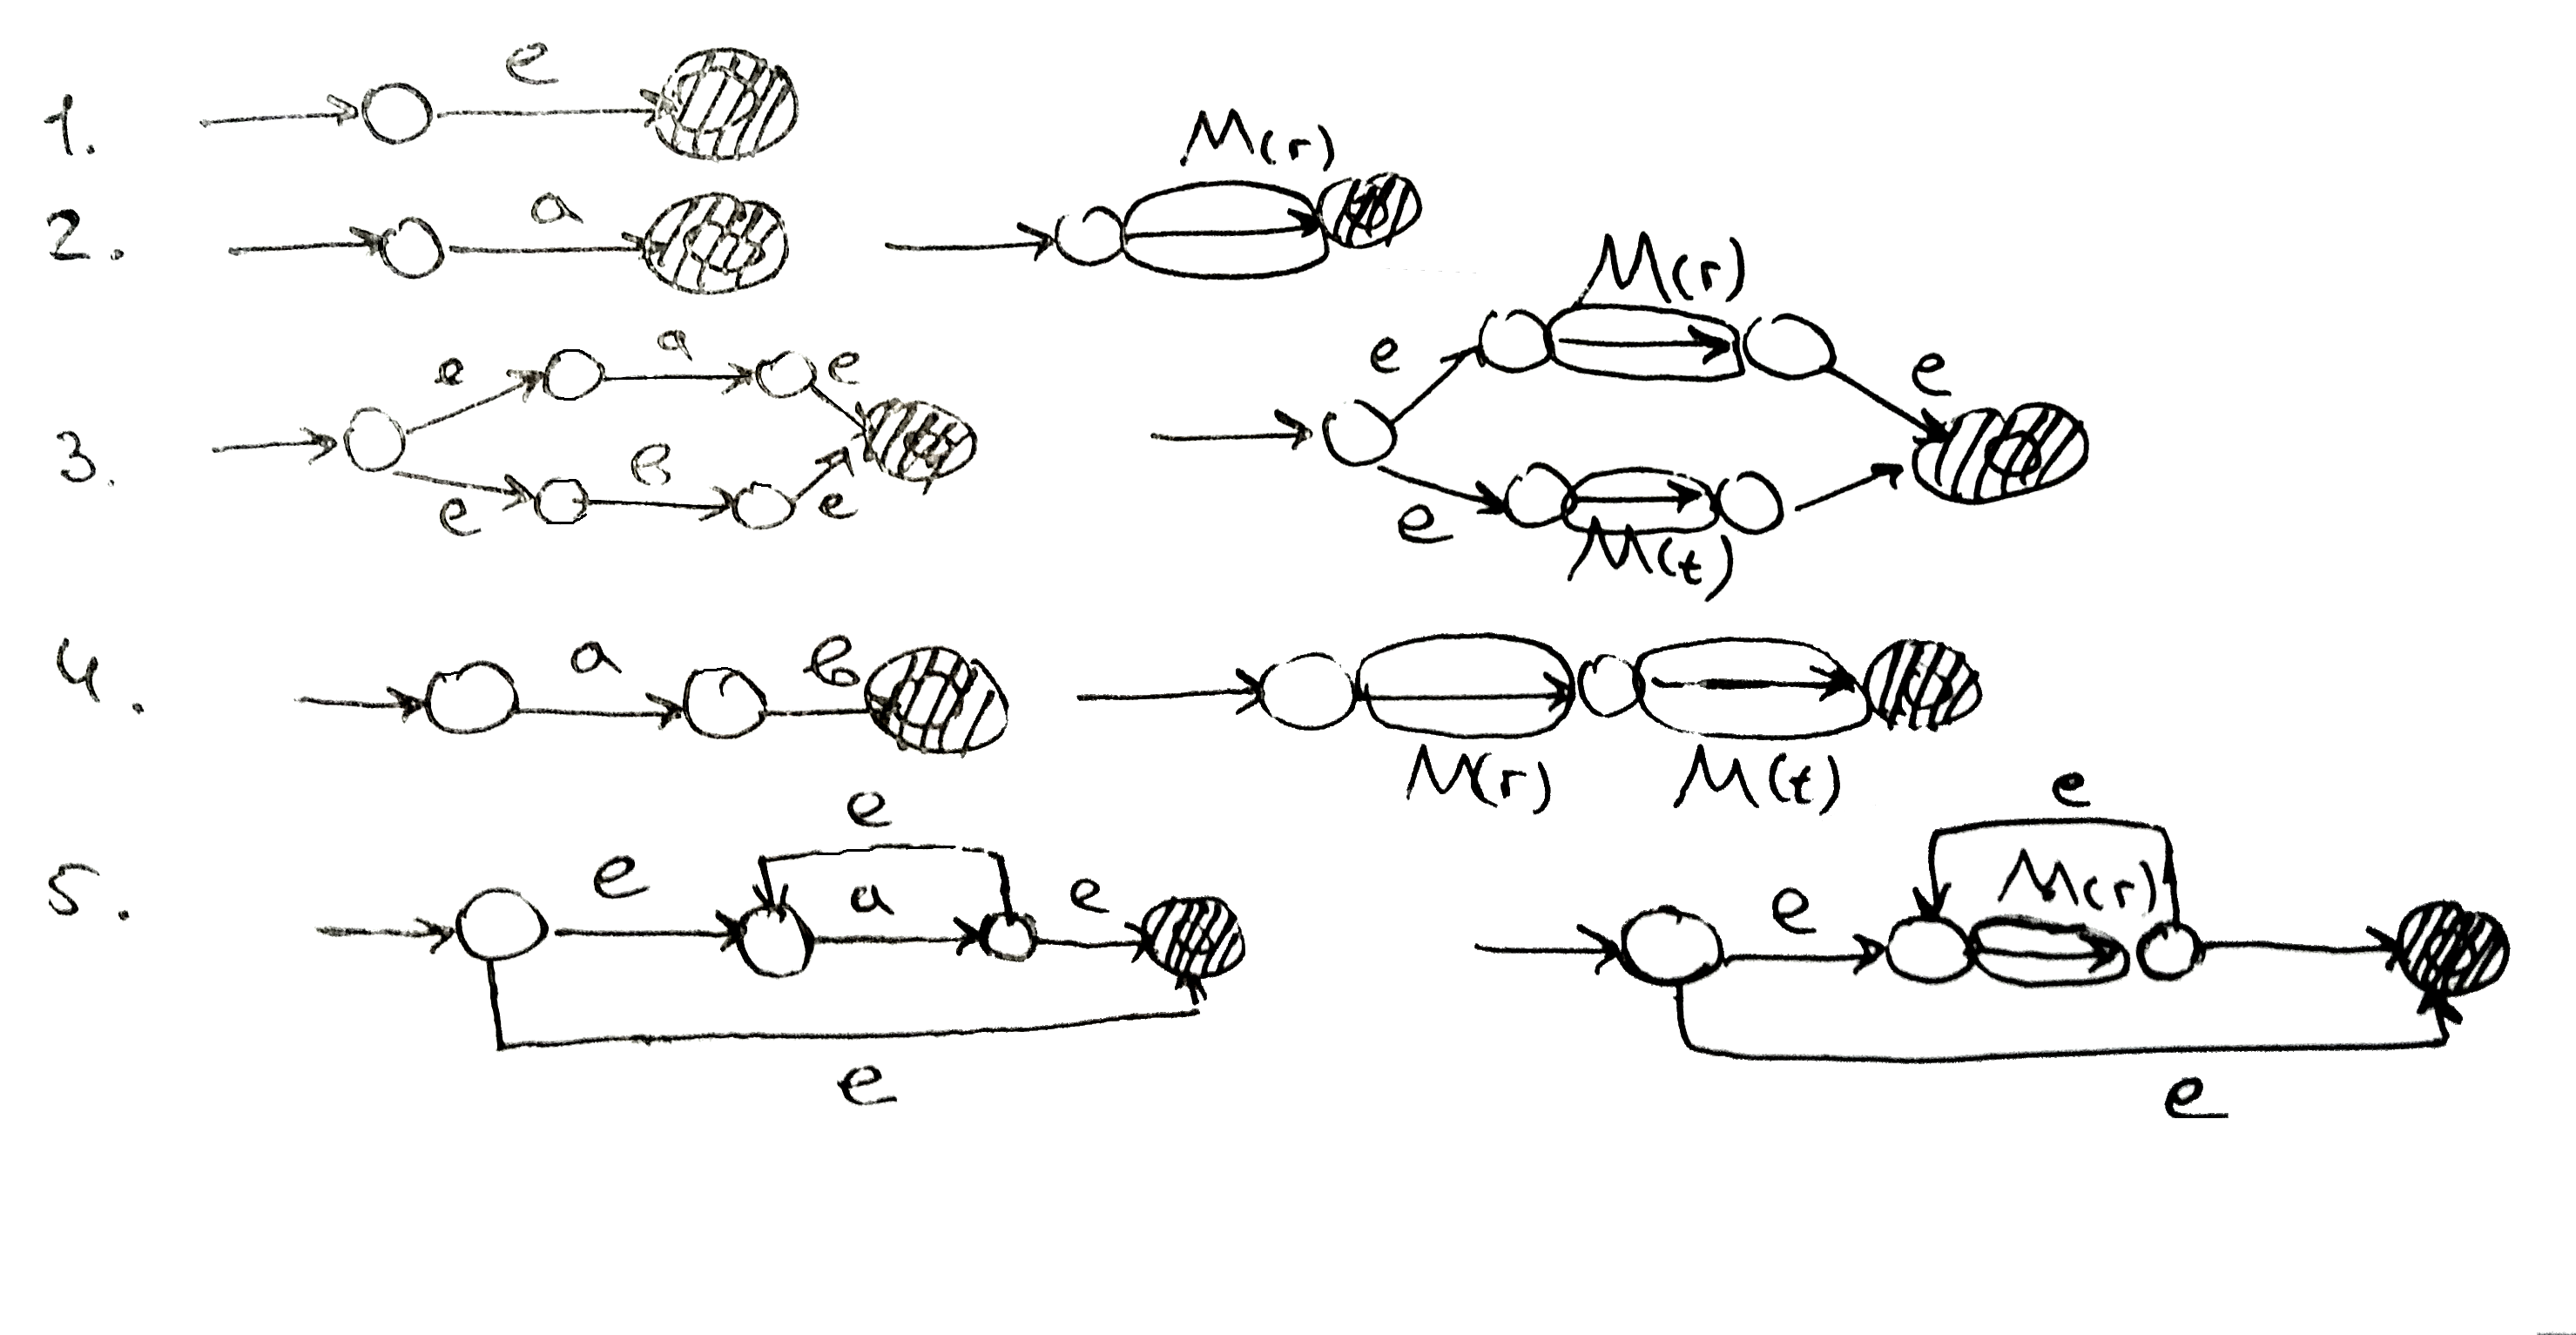
\includegraphics[scale=0.15]{data/pic1_1.png}\\\\\\\\
	На рисунке изображено построение НКА для РВ $b(a|ba)*|aab$\\
	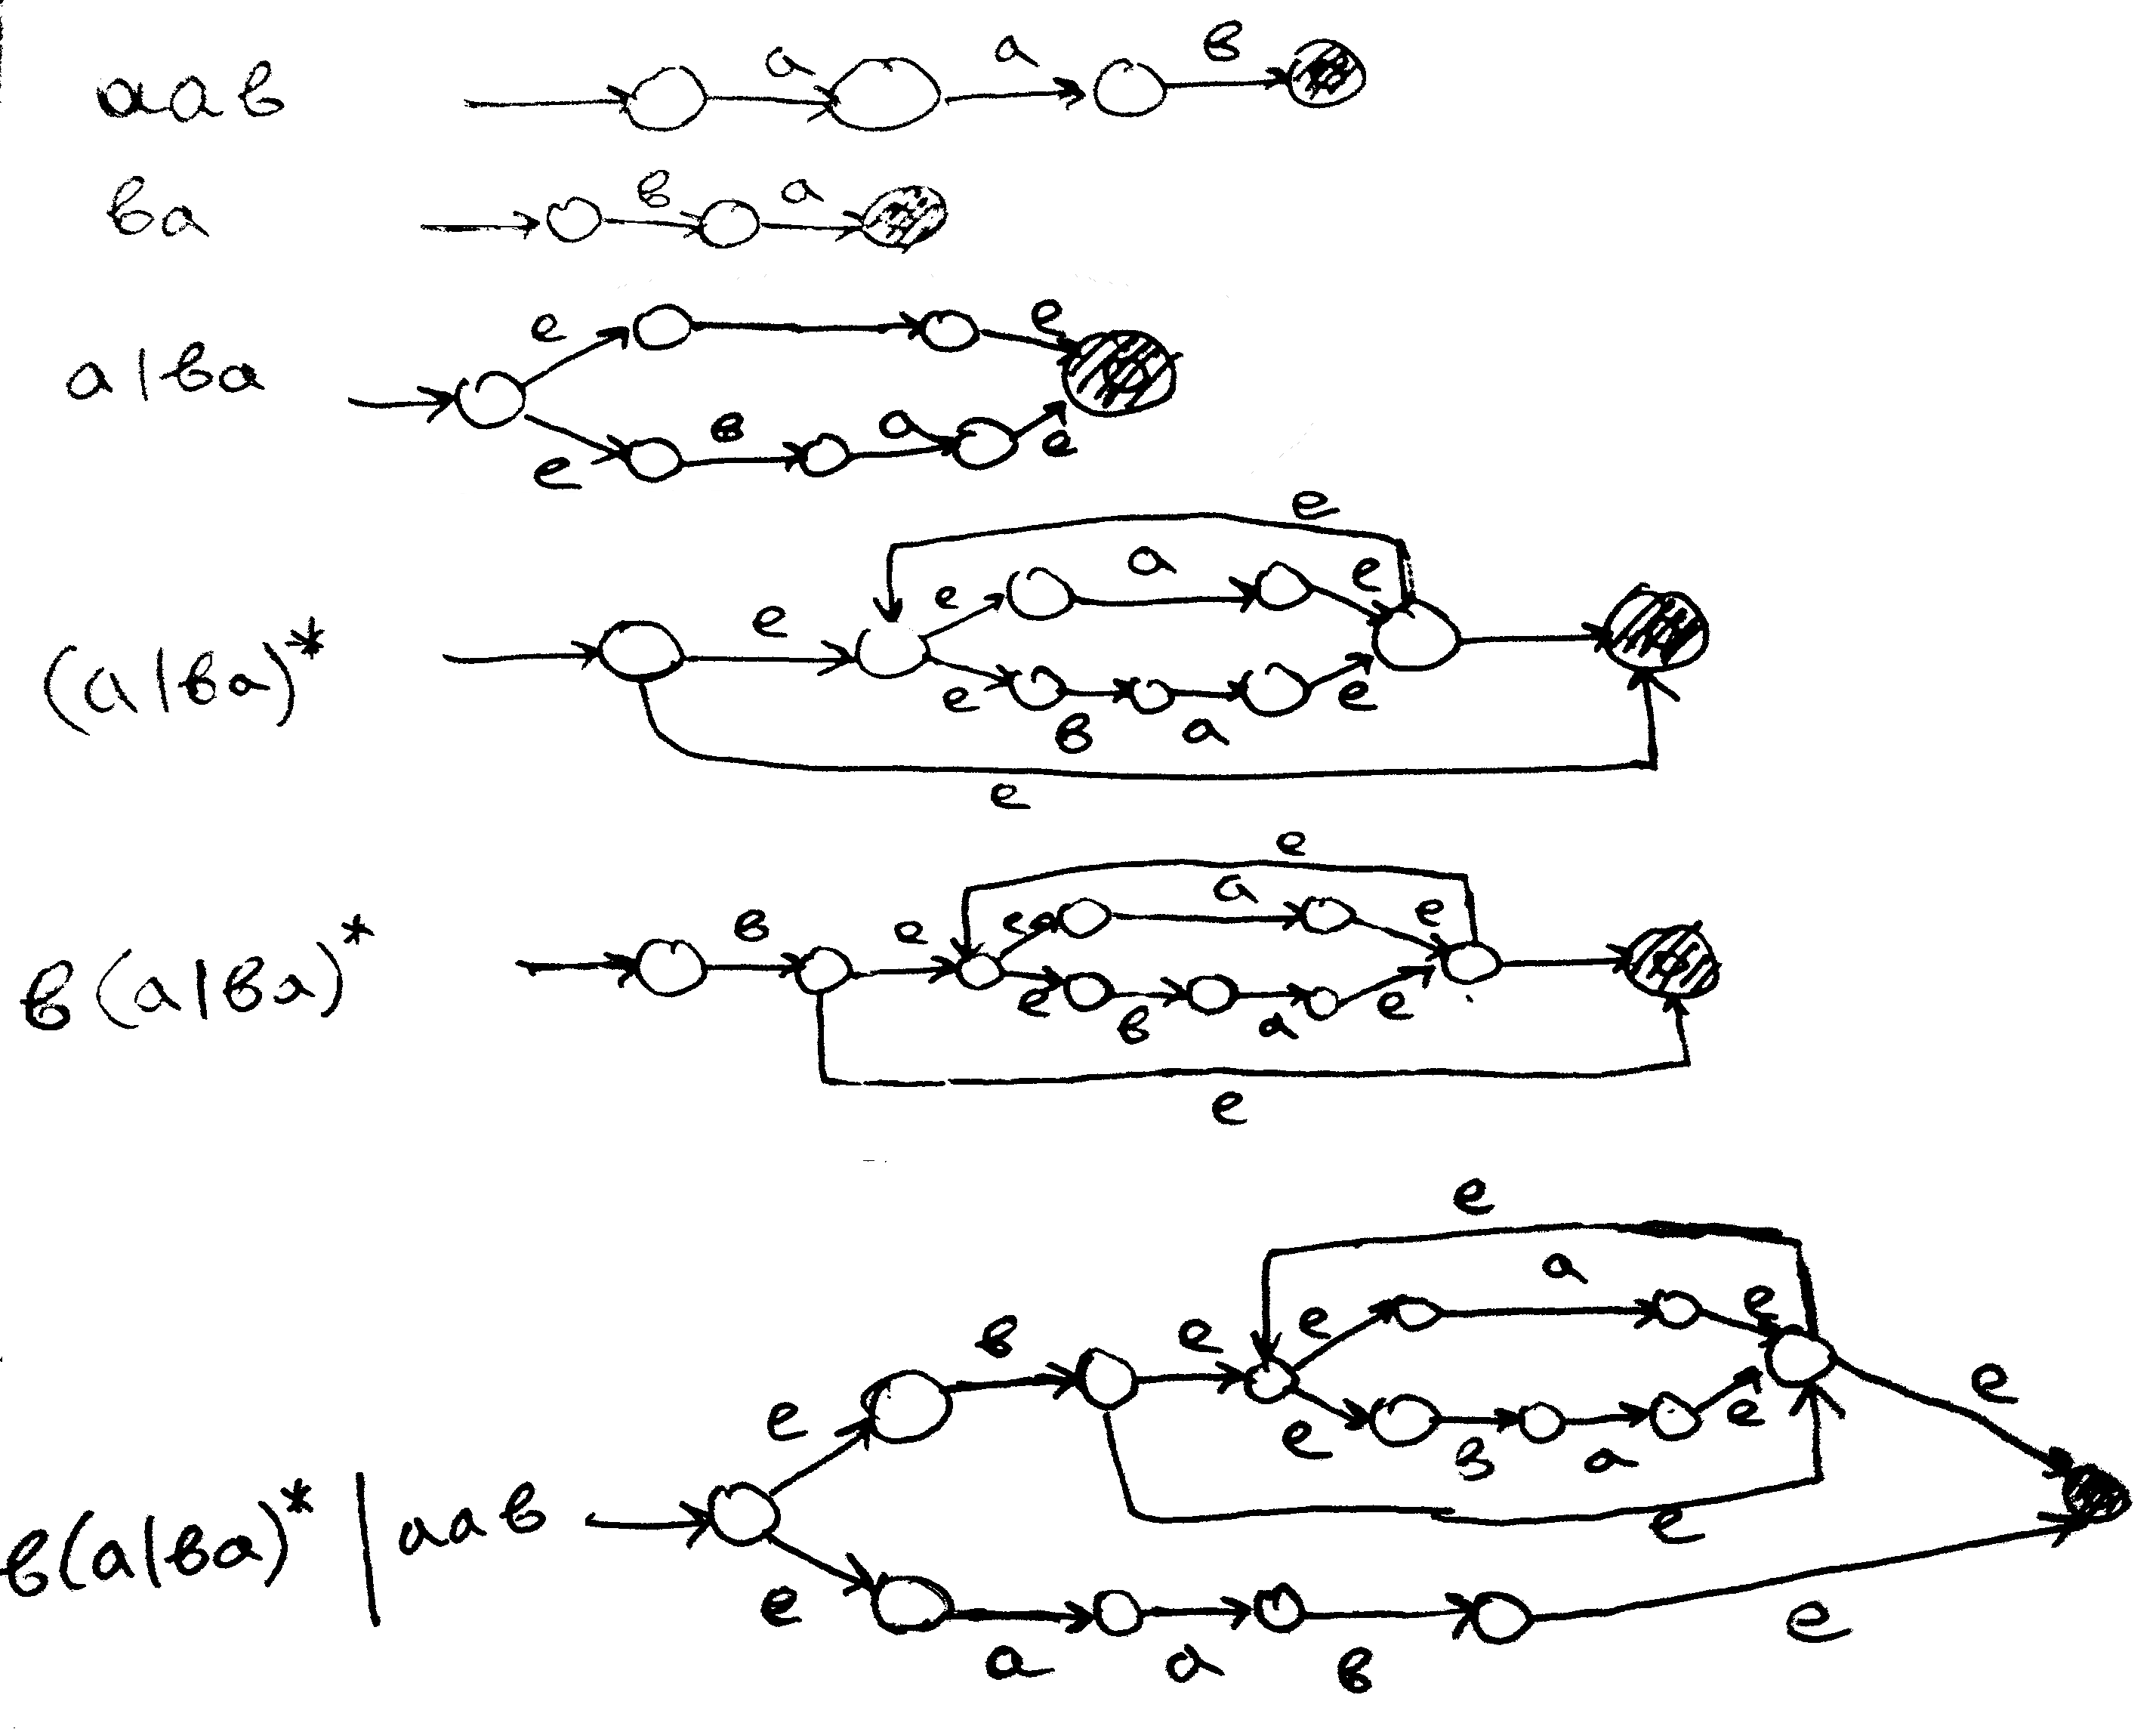
\includegraphics[scale=0.15]{data/pic1_2.png}\\
	\section{Почему это работает}
	Правильность таких построений довольно очевидна, но если не верится, можно походить по
	полученным НКА по дугам и убедиться, что ничего кроме того, что описано в РВ, по ним
	составить нельзя.
	\newpage
	
	\chapter{ДКА по НКА}
	Глядя на НКА, полученные по РВ может показаться, что там слишком много лишних e-переходов,
	и они бесят. Также НКА это вам не ДКА: есть неопределенности которые бесят (хотя процесс
	детерминирования бесит больше). В любом случае существует алгоритм, позволяющий из большого,
	но красивого НКА получить маленький и очень некрасивый ДКА.
	\section{Алгоритм}
	Введем некоторые обозначения:\\\\
	1. $e$-$closure(R)$ (эпсилон-замыкание состояния R) - множество состояний, в которые можно
	попасть из состояния $R$ по символу $e$. Стоит отметить, что "скачков"
	может быть больше одного,
	то есть, если в состояние $Q$ можно попасть из $P$ по $e$, а из $Q$ можно по $e$ попасть в $R$,
	то $R \in e$-$closure(Q)$. На языке умных людей это называется транзитивностью, но я тут не
	сложными словами щеголять пришел.\\\\
	2. $move(R, a)$ (достижимые из $R$ по $a$) - множество состояний, в которые можно попасть из
	состояния $R$ по символу $a$. (тут скачок должен быть только один)\\\\
	В качестве примера рассмотрим уродца из предыдущей главы:\\ $b(a|ba)*|aab$
	\newpage
	1. Для начала все состояния надо пронумеровать\\
	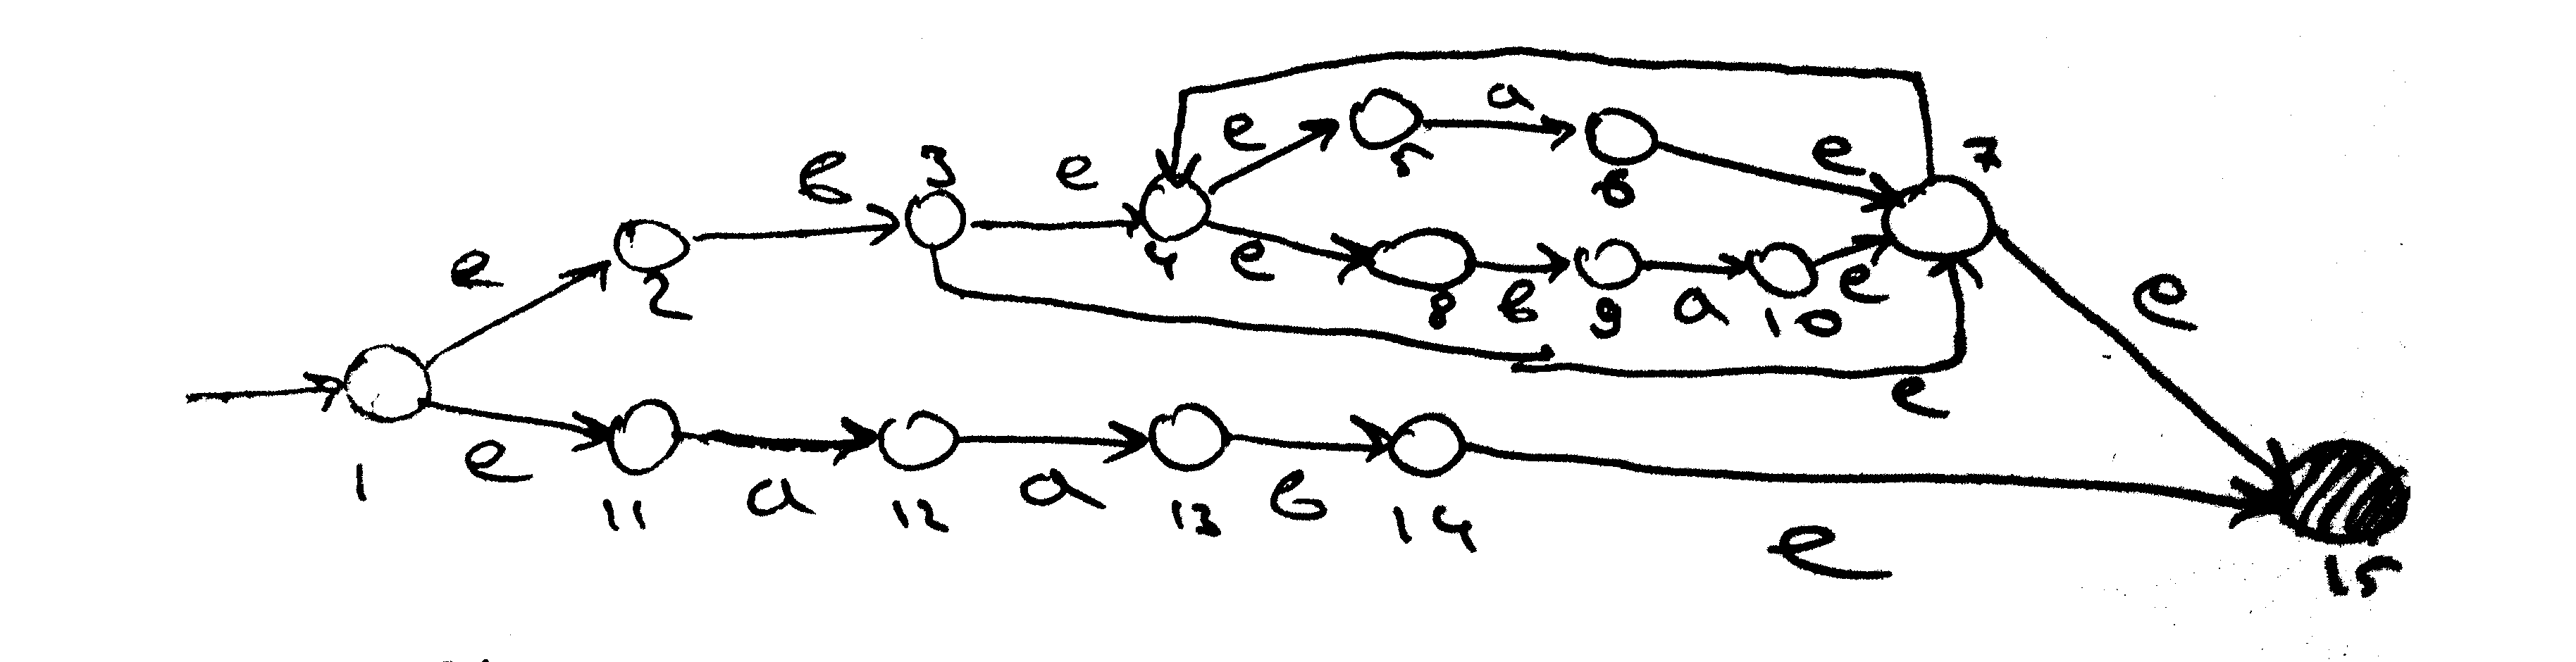
\includegraphics[scale=0.13]{data/pic2_1.png}\\
	Далее мы начинаем описывать новый автомат с новыми состояниями - тут уже традиционно
	используют заглавные латинские буквы. Каждое новое состояние описывается множеством 
	старых состояний из первого автомата.\\\\
	2. В качестве начального состояния нового ДКА берут $A=e$-$closure(1)$, в нашем случае
	это $A=\{1, 2, 11\}$.\\\\
	3. Далее формируются следующие правила переходов:\\
	$D(A, a) = move(A, a)+e$-$closure(move(A, a))$\\
	$D(A, b) = move(A, b)+e$-$closure(move(A, b))$\\
	И т.д.\\\\
	Пусть вышло так, что есть состояние $Q$, из которого по символу $b$ мы переходим в состояние,
	описываемое множеством $\{1, 2, 3, 4, 6, 8, 12, 23\}$. При этом, если у такого множества уже
	есть имя, например $W$, то это попросту значит, что $D(Q, b)=W$. Если такого множества раньше
	не встречалось, то оно добавляется в таблицу состояний нового ДКА.\\
	Звучит сложно и скучно, поэтому лучше посмотреть на живой пример.\\
	$A=\{1, 2, 11\};$\\
	$move(A, a) = move(1, a)+move(2, a)+move(11,a);$\\
	$move(A,a)=\{\}+\{\}+\{12\}=\{12\};$\\
	$e$-$closure(move(A, a))=\{\};$\\
	$D(A, a) = move(A, a)+e$-$closure(move(A, a))=\{12\}+\{\}=\{12\};$\\
	Состояния $\{12\}$ у нас еще не было, поэтому добавим его в таблицу состояний и назовем его
	$B$.\\
	Проделаем аналогичные выкладки для символа $b$.\\
	$move(A, b) = move(1, b)+move(2, b)+move(11,b);$\\
	$move(A, b) = \{\}+\{3\}+\{\}=\{3\};$\\
	$e$-$closure(move(A, b))=\{4, 5, 7, 8, 15\};$\\
	$D(A, b) = move(A, b)+e$-$closure(move(A, b))=\{3\}+\{4, 5, 7, 8, 15\}=
	\{3, 4, 5, 7, 8, 15\};$\\
	Состояния $\{3, 4, 5, 7, 8, 15\}$ у нас тоже еще не было, поэтому запишем его в таблицу
	состояний ДКА.\\
	Подобные вычисления надо проводить для каждого символа в алфавите, для каждого нового
	состояния в таблице до тех пор, пока все старые состояния не будут описаны.\\
	С виду может показать, что это очень много писанины, но на деле все эти преобразования
	делаются в уме и единственное, что нужно реально выписывать, это таблицу состояний.\\
	Привожу финальную таблицу переходов для НКА из предыдущей главы.\\
		\begin{tabular}{lcc}
			 & $a$ & $b$ \\
			$A\{1, 2, 11\}$ & $B$ & $C$ \\
			$B\{12\}$ & $D$ & x \\
			$*C\{3, 4, 5, 7, 8, 15\}$ & $F$ & $G$ \\
			$D\{13\}$ & x & $E$ \\
			$*E\{14, 15\}$ & x & x \\
			$*F\{4, 5, 6, 7, 8, 15\}$ & $F$ & $G$ \\
			$G\{9\}$ & $H$ & x \\
			$*H\{4, 5, 7, 8, 10, 15\}$ & $F$ & $G$ \\	
		\end{tabular}\\\\
	Удивленный читатель заметит, что некоторые состояния отмечены звездочками и
	спросит, что это. Отвечаю: звездочками помечены конечные состояния. И это следующее
	правило алгоритма построения:\\\\
	4. Конечными состояниями нового ДКА помечаются такие состояния, которые содержат в себе
	конечное состояние старого НКА.\\
	В данном случае старым конечным состоянием является 15, поэтому все состояния, имеющие в себе
	15 становятся конечными.\\
	На рисунке изображен полученный ДКА.\\
	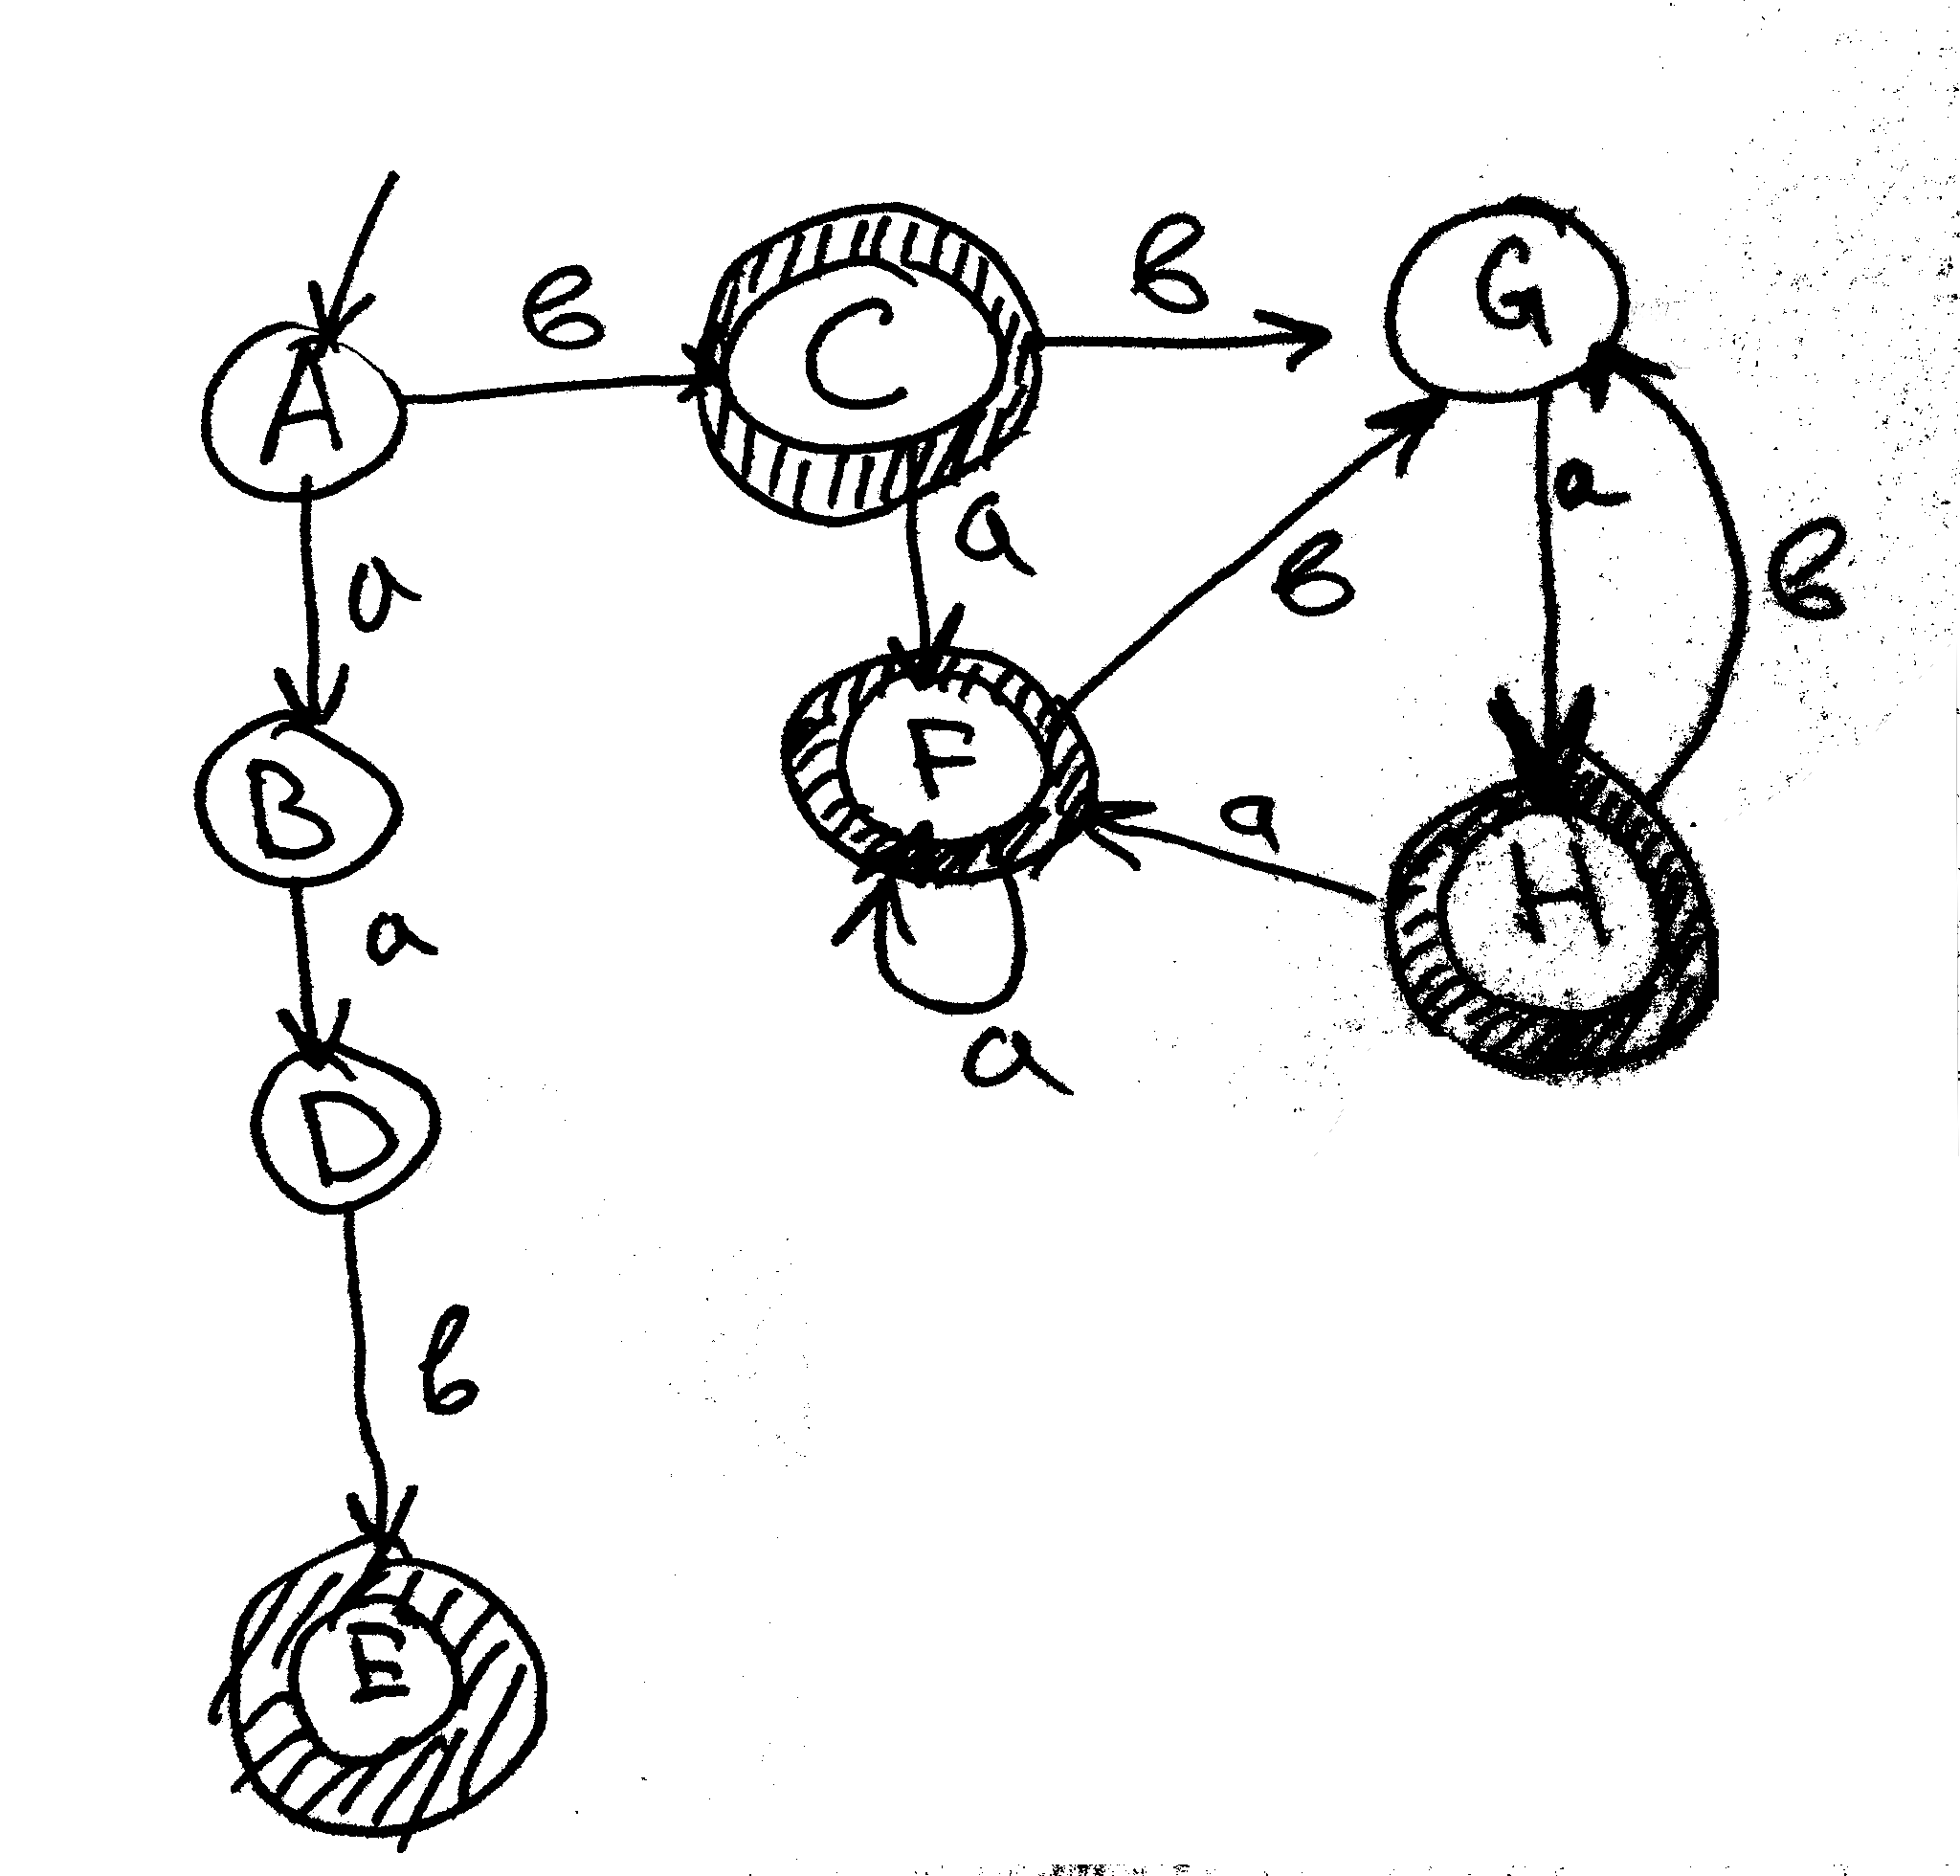
\includegraphics[scale=0.11]{data/pic2_2.png}\\
	\section{Почему это работает}
	Работа алгоритма строится на двух мыслях:\\
	1. Если из одного состояния по $e$ можно перейти в несколько других,
	то зачем нам эти другие состояния, если по сути состояние одно, просто
	разибитое на несколько частей? (незачем)\\
	Грубо говоря, мы стягиваем за $e$-дуги много состояний в одно, как за веревки.\\
	2. Если после стягиваний состояний, две дуги, раньше шедшие в два разных состояния,
	теперь идут в одно стянутое, то действительно ли между этими дугами есть разница? (нет)\\
	\newpage
	\chapter{ДКА по РВ}
	Допустим, что у нас есть РВ, которое необходимо преобразовать в ДКА. И казалось бы, уже есть
	целых 2 алгоритма, с помощью которых это можно сделать: сначала строим НКА, потом по нему же
	ДКА. Но есть более быстрый алгоритм прямого перевода.
	\section{Алгоритм}
	Для начала возьмем все то же РВ из первой главы $b(a|ba)*|aab$\\
	1. Строим расширение РВ: просто дописываем в конце символ конца, как бы странно
	это не звучало. Получаем $(b(a|ba)*|aab)\#$\\\\
	2. Нумеруем все буквы в нашем РВ (в том числе и символ конца)\\
	$(b(a|ba)*|aab)\#$\\
	\hspace*{5pt}$1\ 2\ 34\ \ \ \ \ 567\ 8$\\\\
	\newpage
	3. Строим дерево РВ (обязательно помним про приоритеты операций)\\
	Также на рисунке по бокам от каждого символа стоит его номер в РВ, чуть позже
	будет понятно, зачем.\\\\
	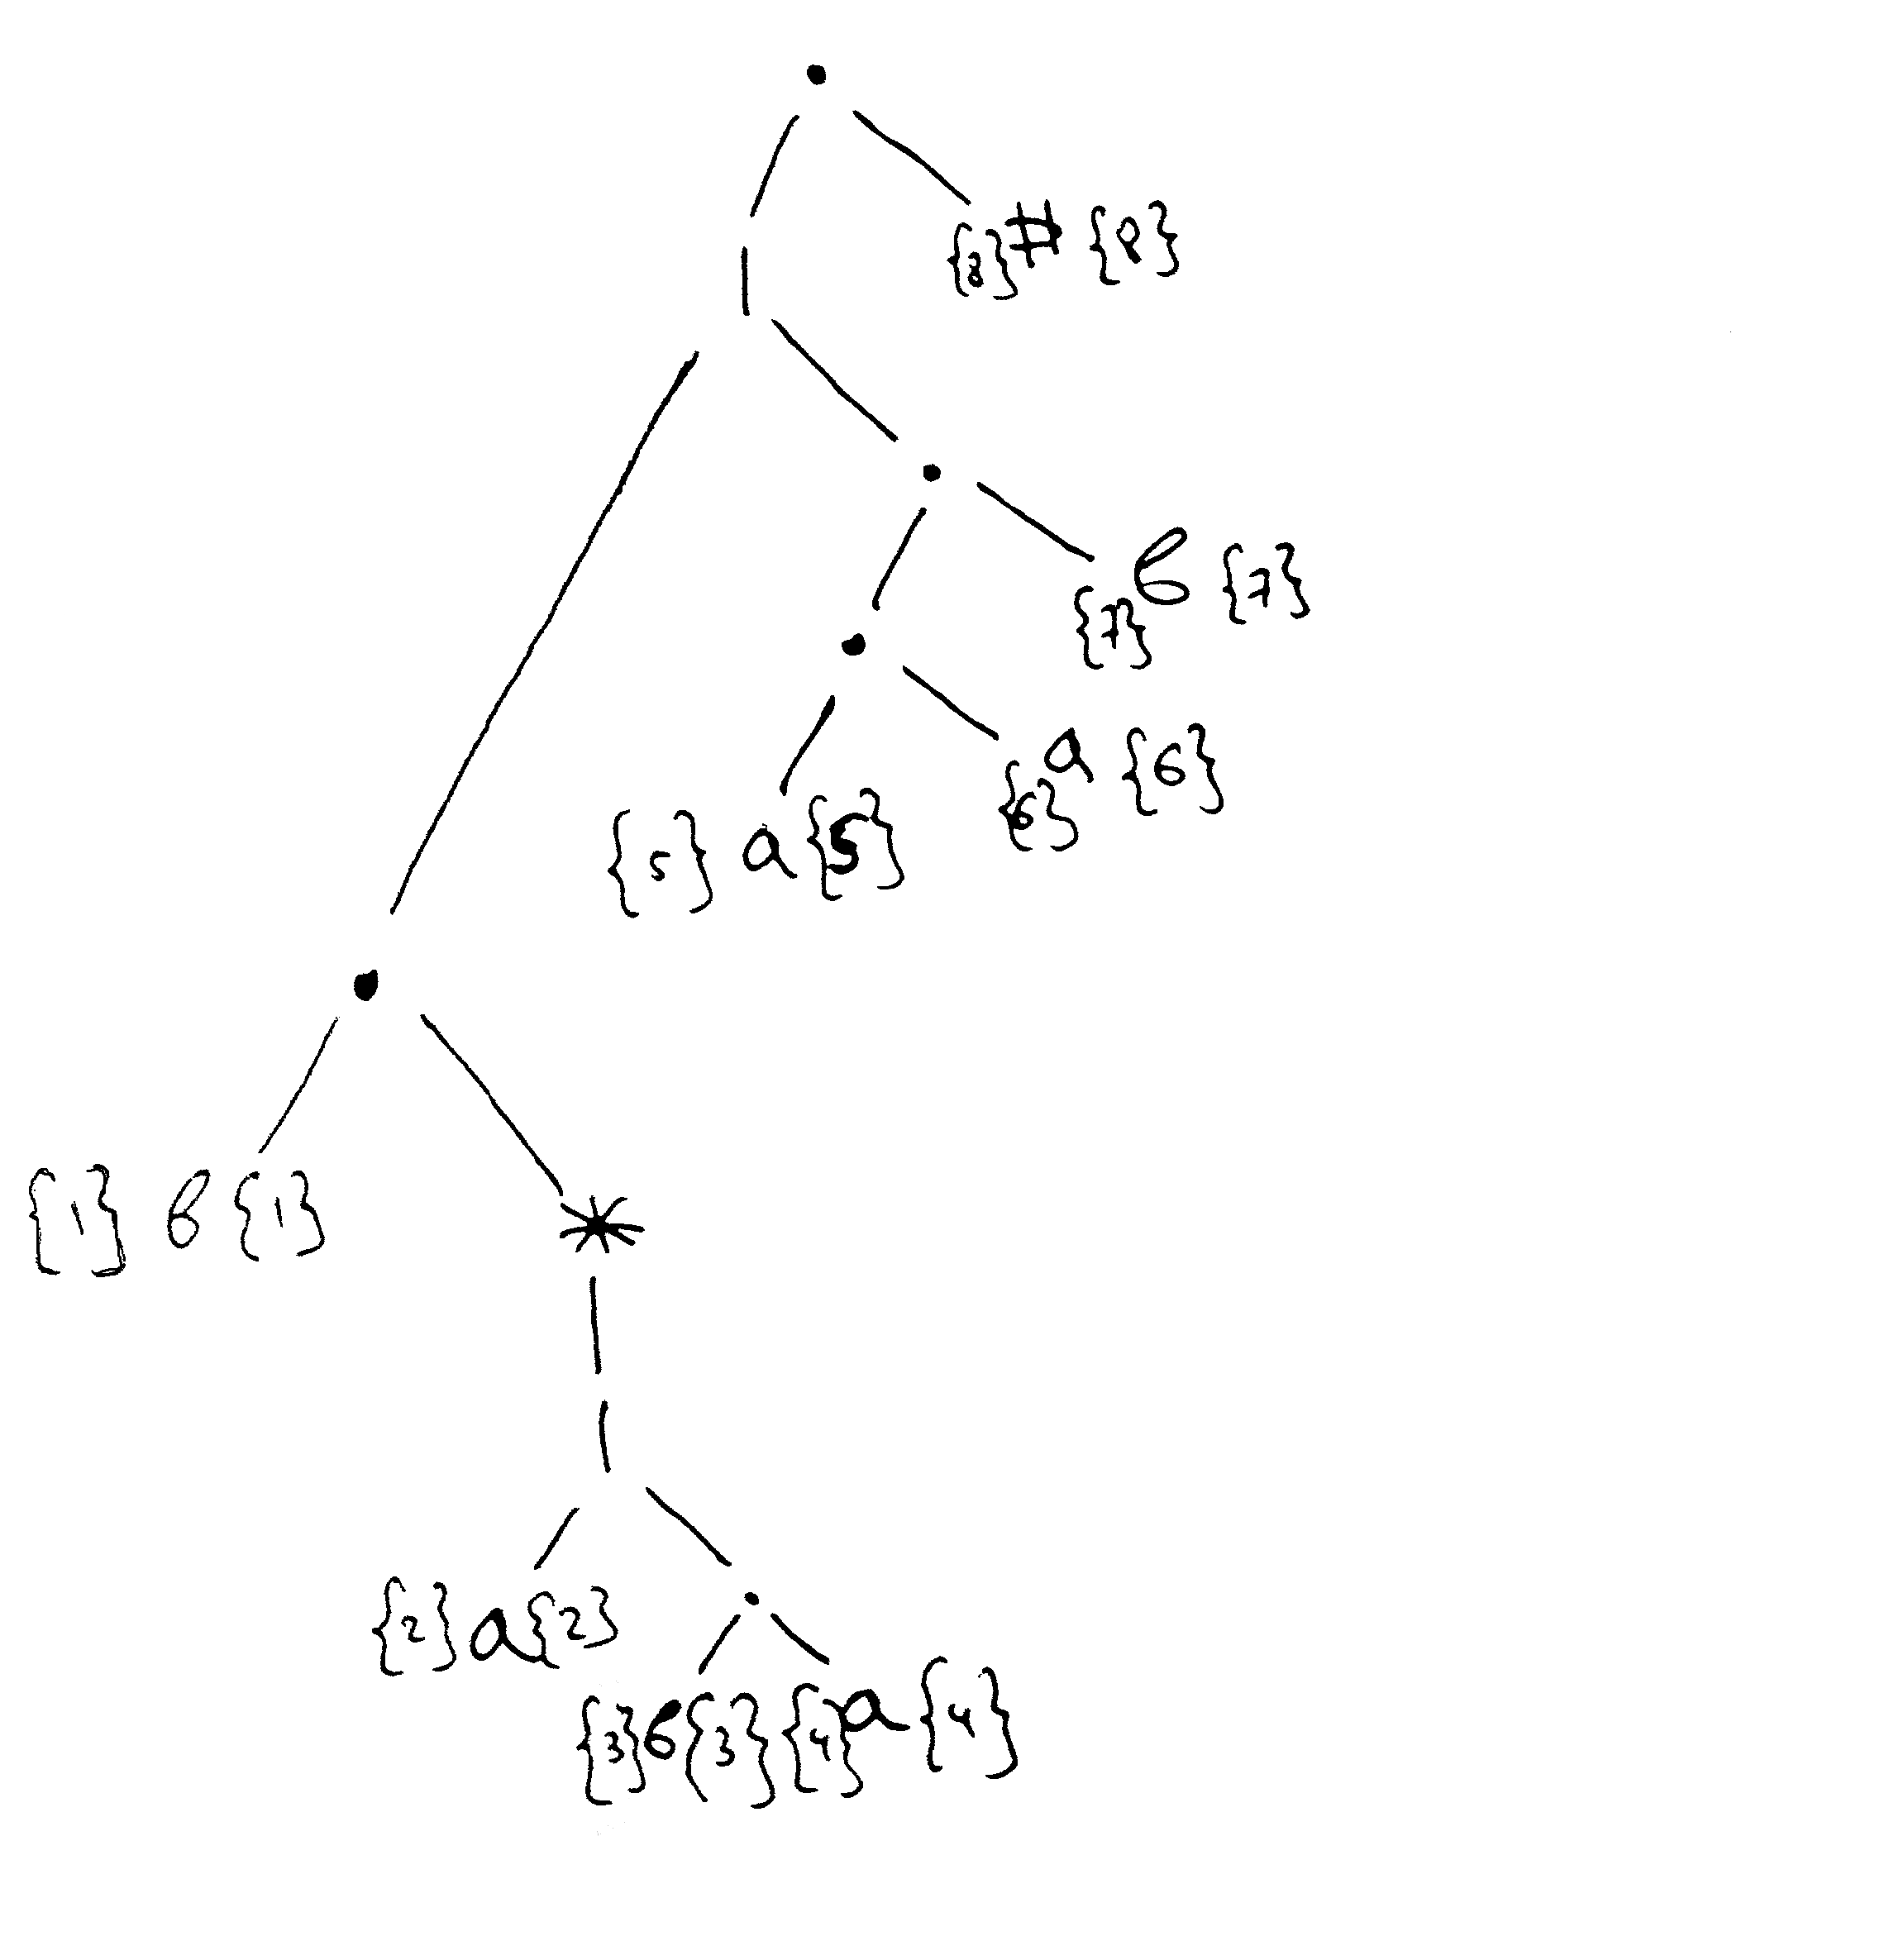
\includegraphics[scale=0.13]{data/pic3_1.png}\\
	4. Теперь пошла жара: надо определить кучу разных множеств для поддеревьев:\\\\
	$nullable(s)$ - обнуляемость: может ли поддерево $s$ породить пустую цепочку\\
	Тут несколько вариантов:\\
	\hspace*{30pt}$s$ - лист дерева: $nullable(s)=false$\\
	\hspace*{30pt}$s=p*$, где $p$ - некоторое поддерево: $nullable(s)=true$\\
	\hspace*{30pt}$s=p\ |\ q$:\ $nullable(s)=nullable(p)\ or\ nullable(q)$\\
	\hspace*{30pt}$s=p \bullet q$:\ $nullable(s)=nullable(p)\ and\ nullable(q)$\\
	$firstpos(s)$ - первый символ: множество символов, которые могут идти первыми
	в цепочке, порожденной поддеревом $s$\\
	\hspace*{30pt}$s$ - лист дерева: $firstpos(s)=\{s\}$\\
	\hspace*{30pt}$s=p*$: $firstpos(s)=firstpos(p)$\\
	\hspace*{30pt}$s=p\ |\ q$: $firstpos(s)=firstpos(p) \cup firstpos(q)$\\
	\hspace*{30pt}$s=p \bullet q$: если $nullable(p)$, то $firstpos(s)=firstpos(p) \cup firstpos(q)$,
	\hspace*{30pt}иначе $firstpos(s)=firstpos(p)$ \\
	$lastpos(s)$ - последний символ: множество символов, на которые может заканчиваться
	цепочка, порожденная поддеревом $s$\\
	\hspace*{30pt}$s$ - лист дерева: $lastpos(s)=\{s\}$\\
	\hspace*{30pt}$s=p*$: $lastpos(s)=lastpos(p)$\\
	\hspace*{30pt}$s=p\ |\ q$: $lastpos(s)=lastpos(p) \cup lastpos(q)$\\
	\hspace*{30pt}$s=pq$: если $nullable(q)$, то $lastpos(s)=lastpos(p) \cup lastpos(q)$,
	\hspace*{30pt}иначе $lastpos(s)=lastpos(q)$ \\\\
	На самом деле все это страшно скучная херня и по большей части решается с помощью метода
	пристального взгляда и более-менее здравого смысла.\\
	Теперь можно пояснить и за странные пометки в предыдущем рисунке: слева стояли $firstpos(s)$,
	а справа - $lastpos(s)$\\
	Cейчас прошлый рисунок будет дополнен аналогичными множествами, но уже не только для листьев.\\
	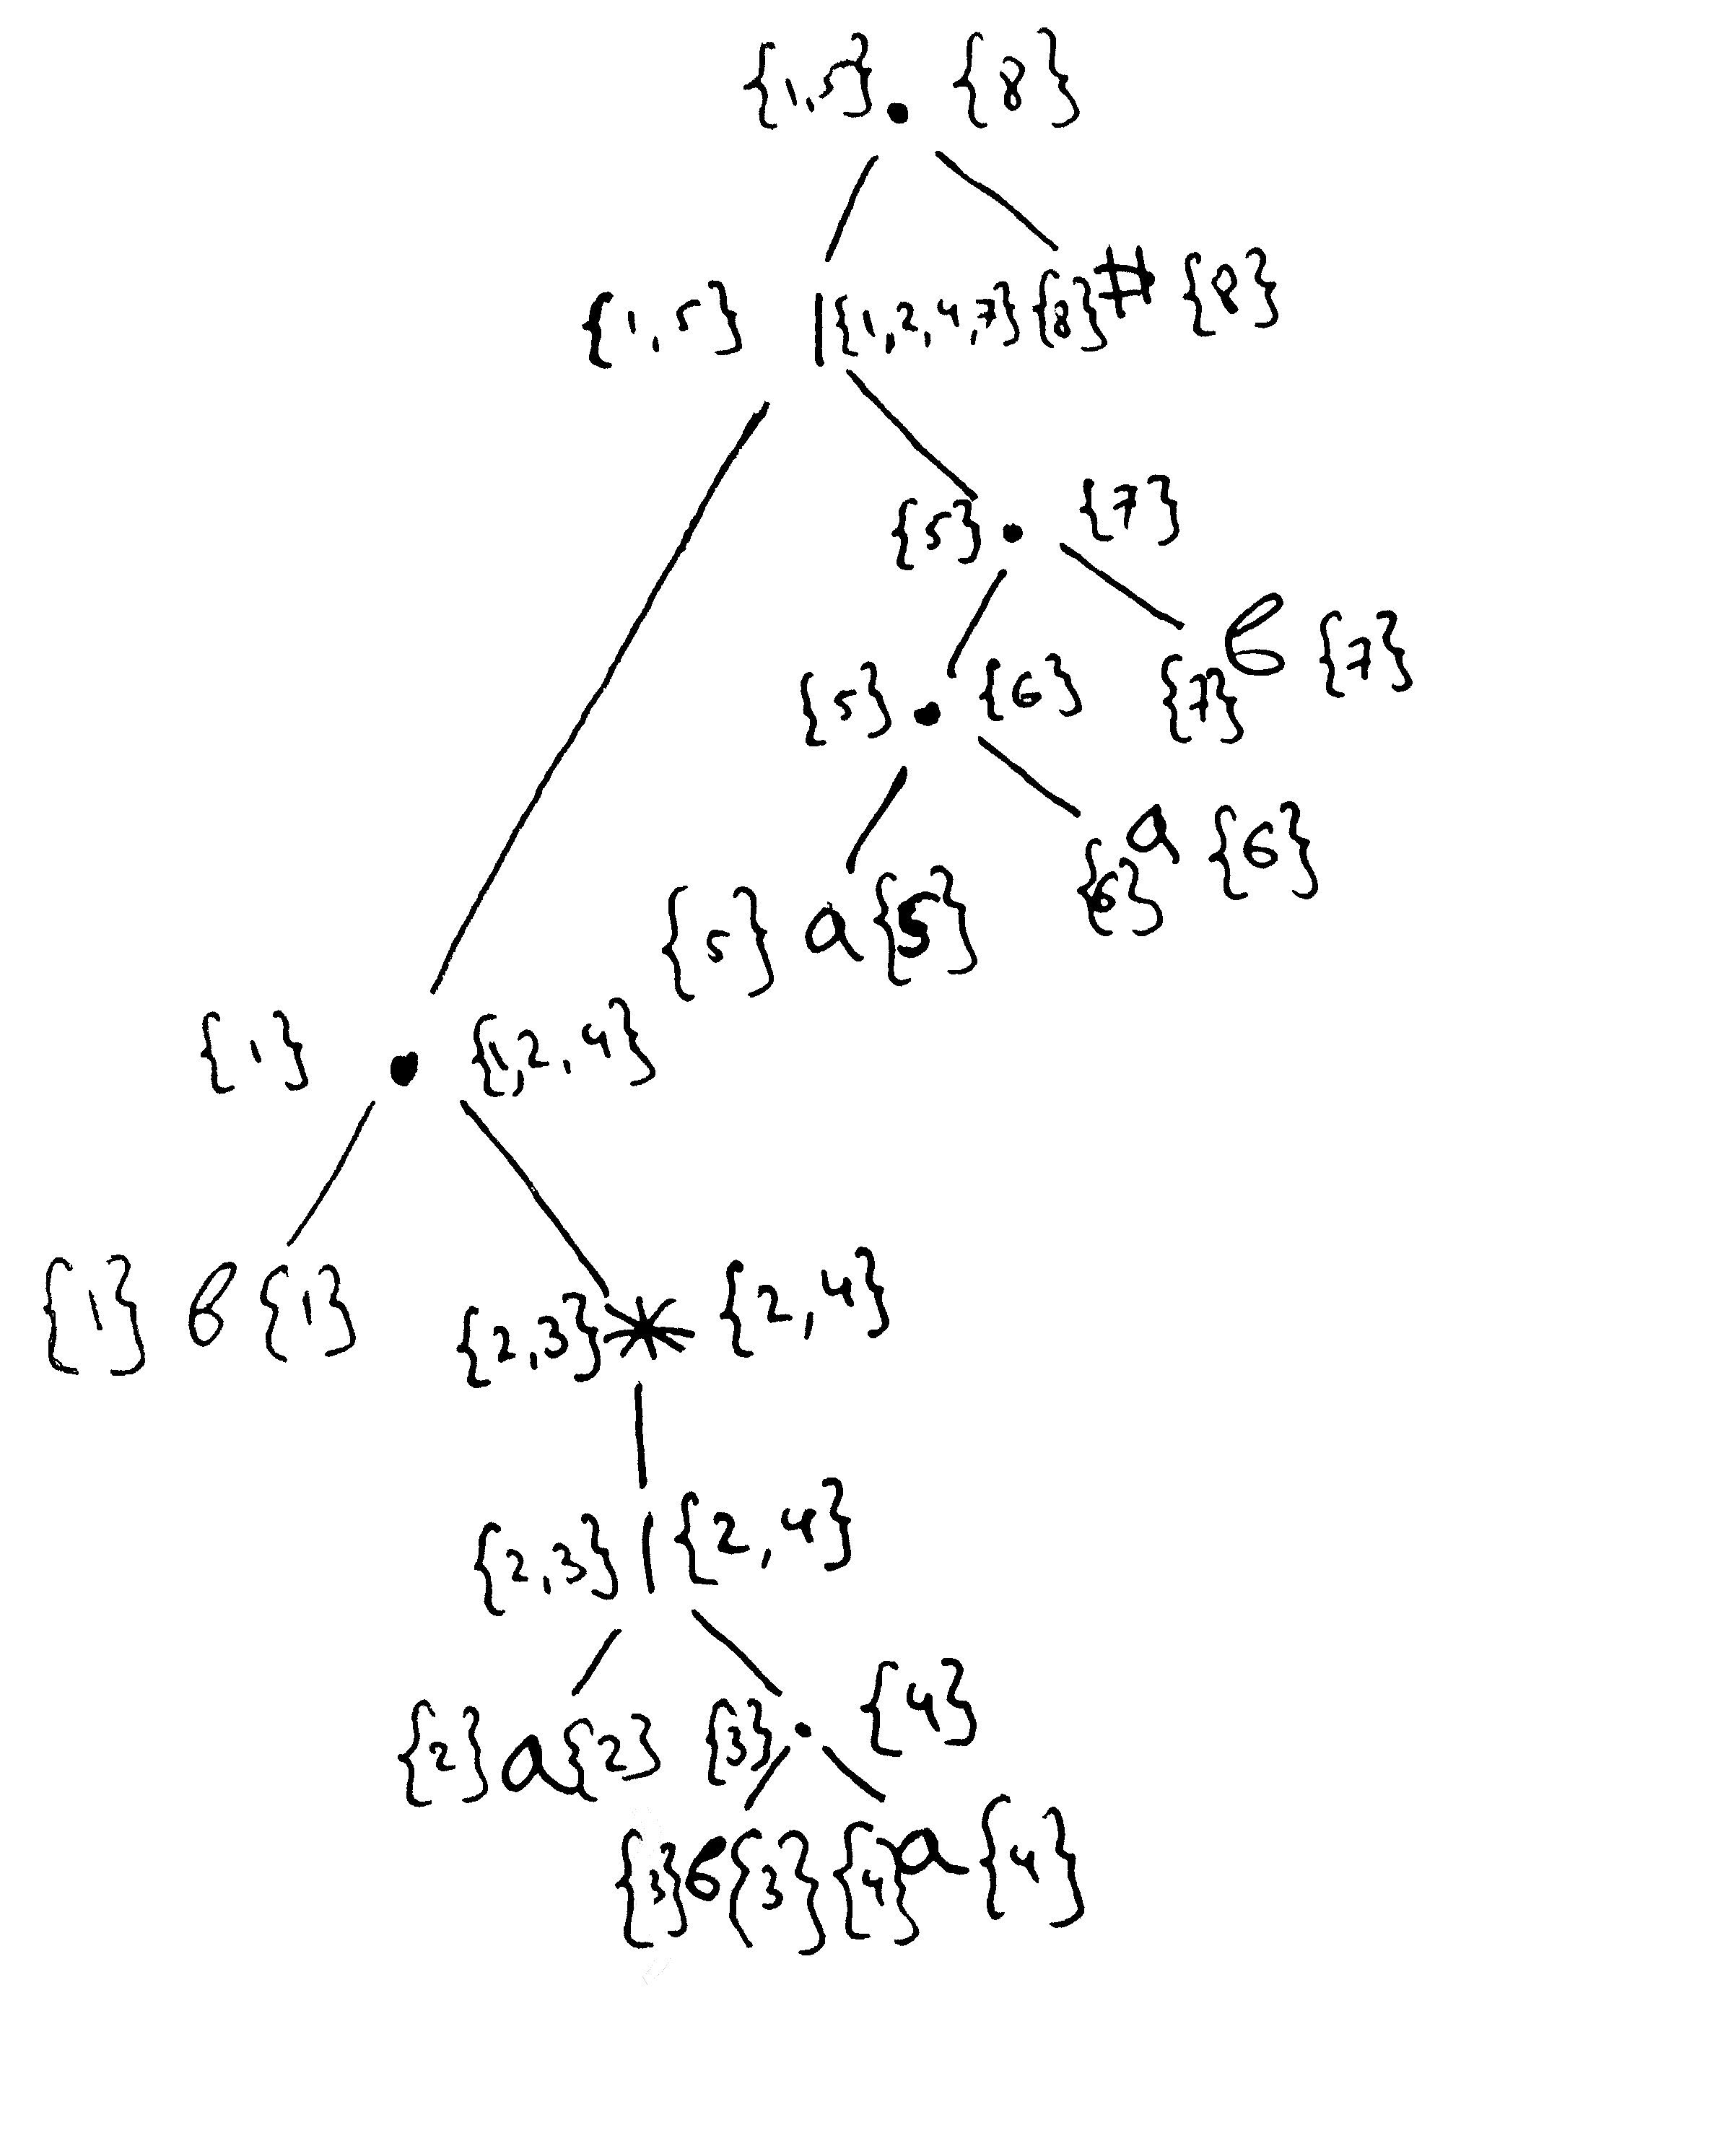
\includegraphics[scale=0.14]{data/pic3_2.png}\\
	5. Жара продолжается: теперь надо вычислить $followpos(s)$ - множество символов, которые могут
	идти прямо после цепочки, порожденной поддеревом $s$.\\
	Здесь строгие алгоритмы выглядят еще скучнее, чем для прошлых множеств, но метод пристального
	взгляда по-прежнему здесь справляется довольно неплохо (хотя иногда и допускает ошибки: мой
	вот пристальный взгляд в свое время накосячил, а теперь я пишу эту методичку).\\
	Но в любом случае, вот алгоритм:\\
	\hspace*{30pt}Для $p \bullet q$: для каждого $i \in lastpos(p)$ добавить $firstpos(q)$
	в $followpos(i)$\\
	\hspace*{30pt}Для  $p*$: для каждой позиции $i \in lastpos(p)$ добавить $firstpos(p)$\\
	\hspace*{30pt}в $followpos(i)$\\
	Если первое правило вполне понятно, то второе уже посложнее. Оно становится понятнее,
	если напомнить себе, что из $p*$ может получиться цепочка $pp$. Тогда все встает на
	свои места (потому что явным образом видно, что за всеми $lastpos(p)$ спокойно могут
	идти любые символы из $firstpos(p)$. Осозновая это, вы, наверное, не накосячите так,
	как однажды это сделал я.\\
	Для нашего дерева получается такая таблица:\\
		\begin{tabular}{ll}
			 $symbol$ & $followpos(symbol)$ \\
			 1 & $\{2, 3, 8\}$ \\
			 2 & $\{2, 3, 8\}$ \\
			 3 & $\{4\}$ \\
			 4 & $\{2, 3, 8\}$ \\
			 5 & $\{6\}$ \\
			 6 & $\{7\}$\\
			 7 & $\{8\}$\\
			 8 & $\{\}$\\
		\end{tabular}\\
	6. Строим таблицу переходов. Состояния здесь описываются множествами, как и в прошлой главе.
	За начальное состояние $A$ берется множество $firstpos($корень дерева$)$.\\
	Дальше правила переходов описываются следующим образом:\\
	$D(Q, s) = \bigcup\limits_{i=Q \cap s}followpos(i)$\\
	Сложная формула, за которой хрен пойми какая логика стоит, поэтому рассмотрим на живом
	примере:\\
	В данном случае наше стартовое состояние $A=\{1, 5\}$.\\
	Символ $a=\{2, 4, 5, 6\}$(множество	цифр, которые в пронумерованном РВ 
	стоят под символом $a$)\\
	Пересекая множества $a$ и$A$ получим $\{5\}$. $followpos(5)$ смотрим по таблице -
	$\{6\}$. Такого множества в качестве состояния у нас еще не было, поэтому назовем его
	$B=\{6\}$. Таким образом получается, что $D(A, a) = B$.\\
	Абсолютно аналогично поступаем со всеми символами алфавита и всеми неописанными множествами.
	Со временем новые состояния перестанут поступать, а мы получим законченную таблицу.\\
	Конечным состоянием объявляется то, которое в своем множестве содержит номер символа конца.\\
	\newpage
	Для нашего $b(a|ba)*|aab$ получается следующая таблица:\\
		\begin{tabular}{lcc}
			 & $a\{2, 4, 5, 6\}$ & $b\{1, 3, 7\}$ \\
			 $A\{1, 5\}$ & $B$ & $C$ \\
			 $B\{6\}$ & $D$ & x \\
			 $*C\{2, 3, 8\}$ & $C$ & $E$ \\
			 $D\{7\}$ & x & $F$ \\
			 $E\{4\}$ & $C$ & x \\
			 $*F\{8\}$ & x & x \\
		\end{tabular}\\
	Осталось всего ничего: построить сам ДКА по таблице\\
	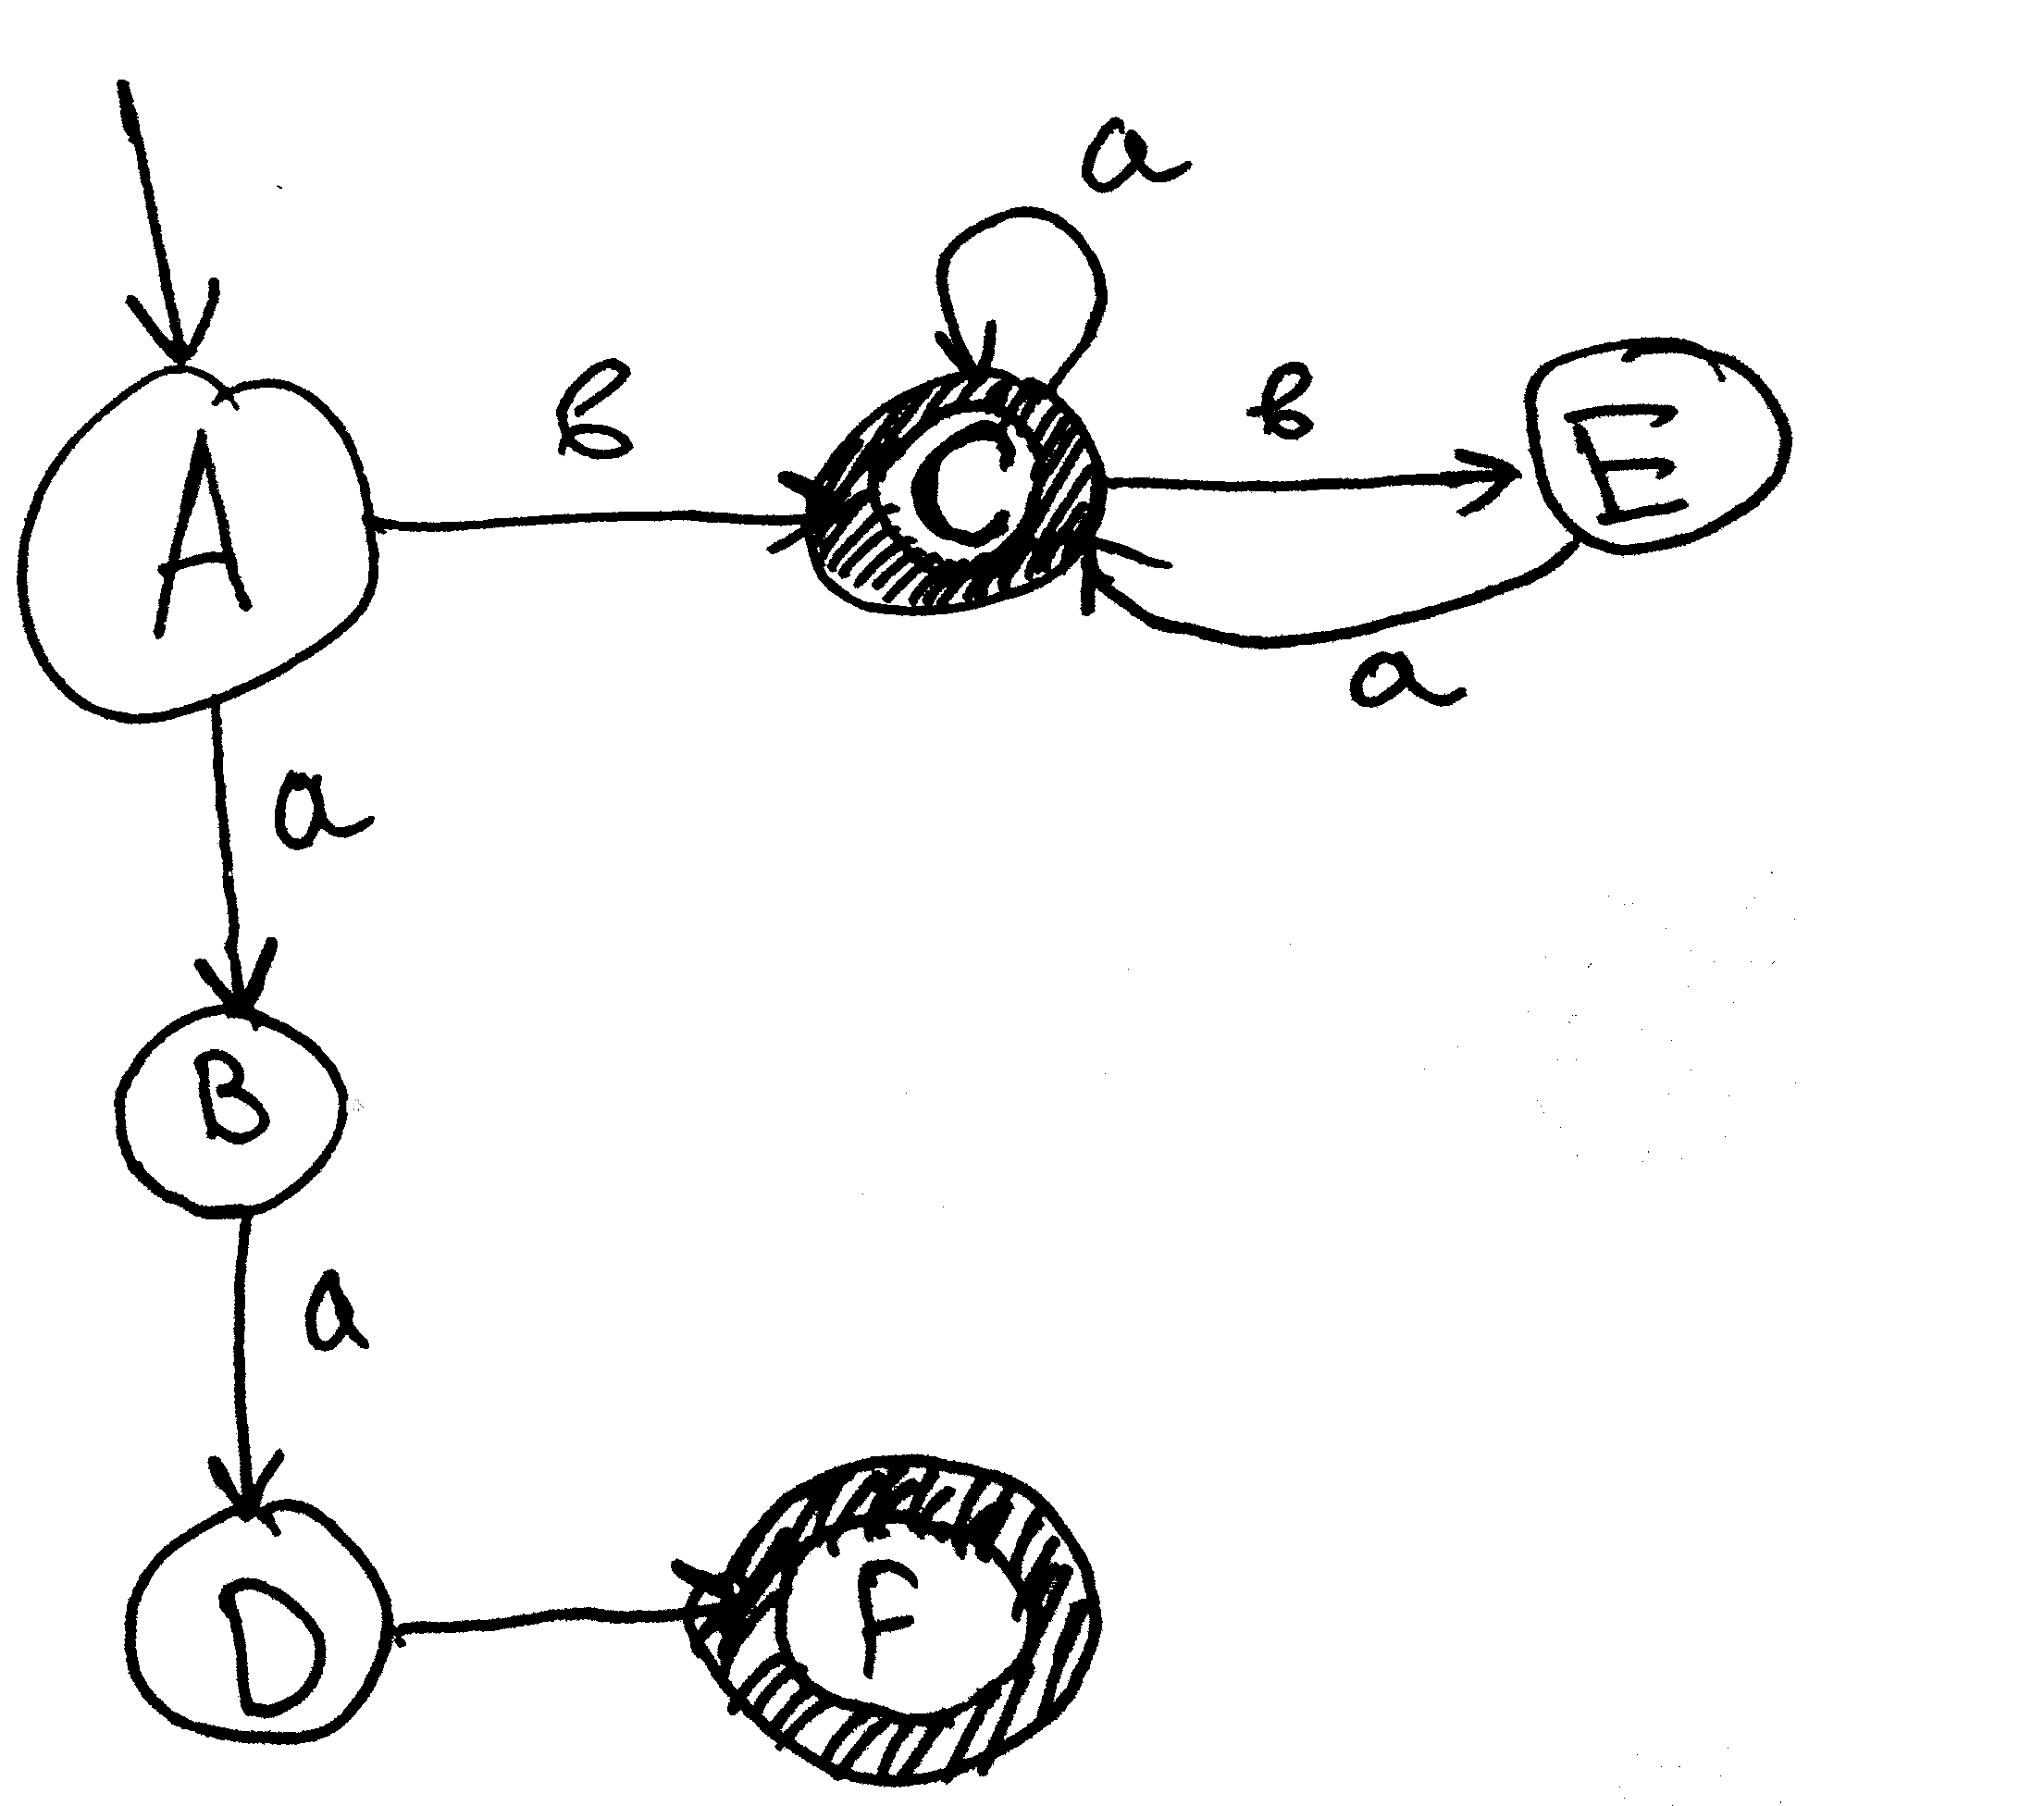
\includegraphics[scale=0.11]{data/pic3_3.png}\\
	\section{Почему это работает}
	По сути каждое состояние описано множеством тех номеров букв, которые могут нас из
	этого состояния вывести. Действительно, если внимательно посмотреть на наше РВ,\\
	$(b(a|ba)*|aab)\#$\\
	\hspace*{5pt}$1\ 2\ 34\ \ \ \ \ 567\ 8$\\
	можно заметить, что выйти из начального состояния мы можем только по буквам $b1$ и $a5$.
	При этом те же буквы, но с другими номерами нам не подойдут. $followspos$-ы здесь тоже
	появляются вполне по делу: через них очень удобно описываются те номера букв, которые выводят
	нас из состояния, в котором мы оказались. Ведь если мы уже прошли вперед по символу $b1$, то
	дальше в цепочке, удовлетворящей РВ, мы по определению сможем встретить только символ из
	$followpos(b1)$.\\
	Из всех этих номеров можно построить очень простой, но здоровый автомат разбора, где алфавит
	нетерминалов будет состоять из чисел, которыми нумеруются буквы в исходном РВ. Просто этот
	большой автомат потом можно будет сократить, заменив номера, на буквы, которые им
	соответствуют.
	\newpage
	\chapter{Минимизация ДКА}
	Недоумевающий читатель мог задаться вопросом: как же так получилось, что мы взяли
	одно РВ, и получилось 2 разных ДКА? И почему это второй ДКА получился таким аккуратным?\\
	А все потому, что ДКА из НКА мы не минимизировали.
	\section{Алгоритм}
	1. Первым делом автомат надо дополнить, то есть, сделать так, чтобы в нем всегда было куда
	перейти (сделаем так, чтобы не было правил вида $D(Q, s) = \O$)\\
	Если автомат уже полный, то ничего не делаем, в противном случае добавляем новое состояние
	$V$ (ну или как вы его назовете, я называю $V$ от слова $void$, потому что это удобно), а
	после этого ведете в него все отсутствующие дуги (и из $V$ в себя же по всем буквам
	алфавита).\\
	В качестве примера возьмем нашего старого доброго уродца из "НКА по РВ" и дополним его:\\
	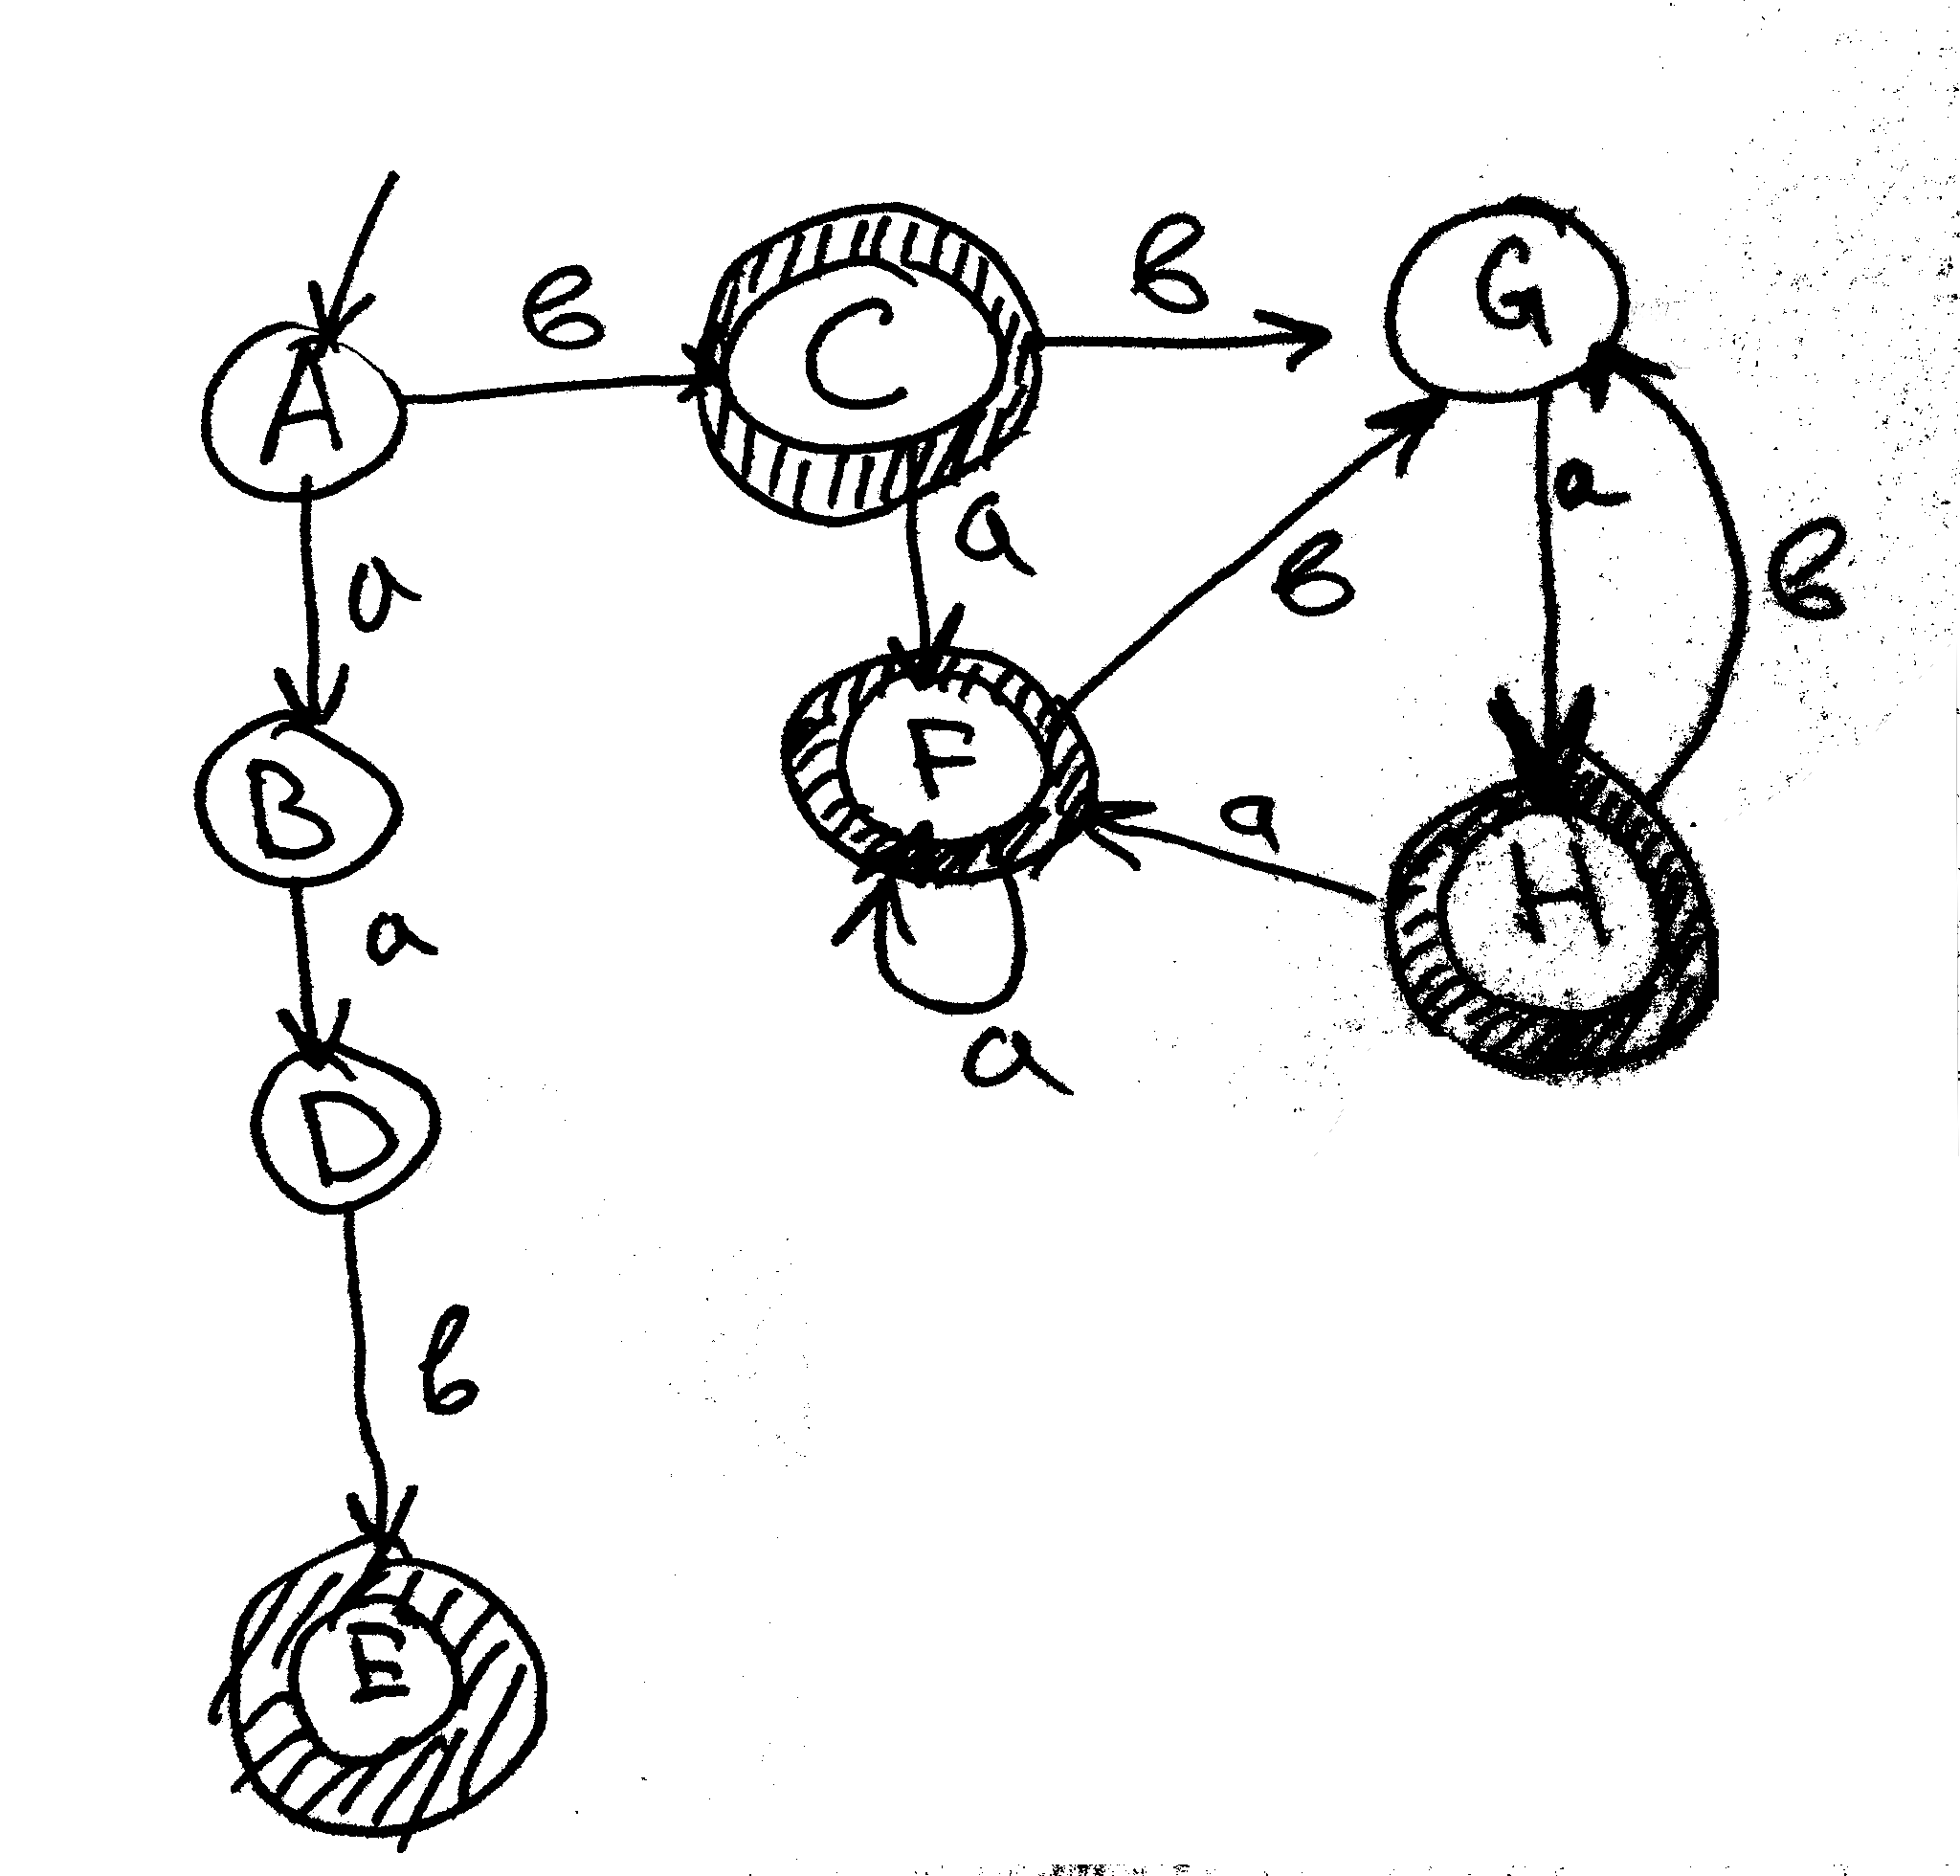
\includegraphics[scale=0.1]{data/pic2_2.png} 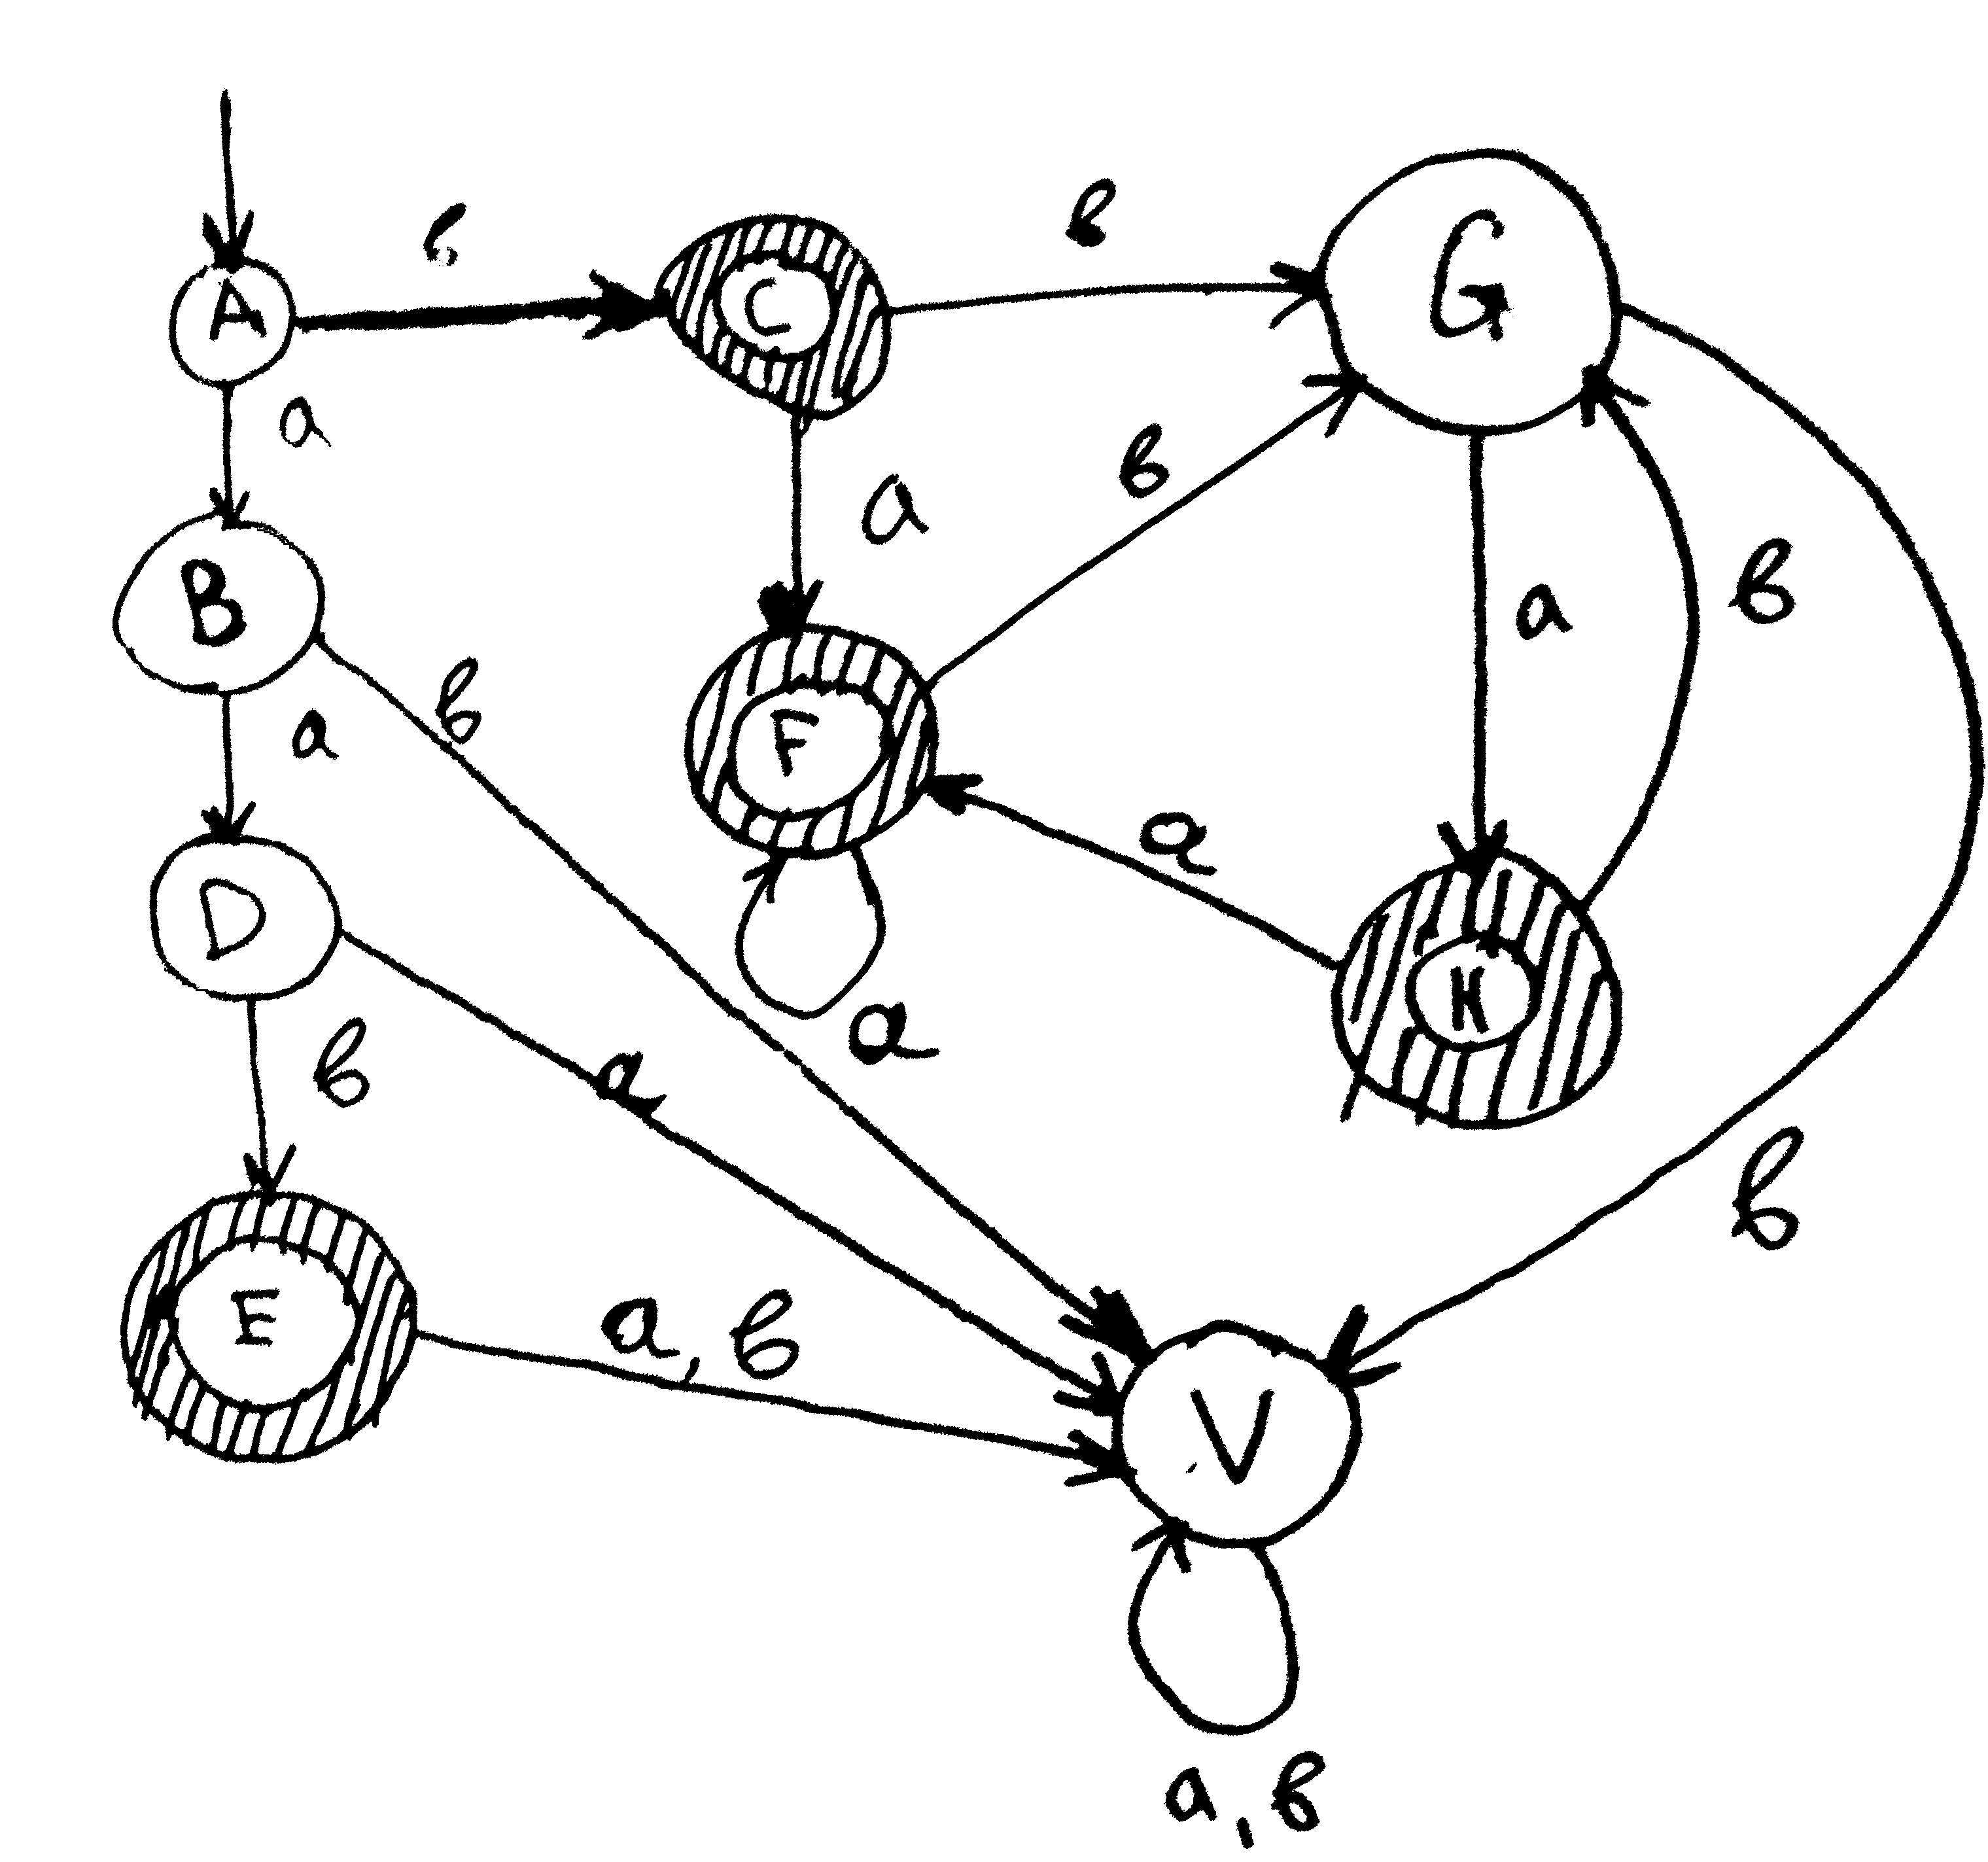
\includegraphics[scale=0.08]{data/pic4_1.png}
	\\\\
	2. Строим разбиение $P_{0}$ множеств состояний следующим образом:\\
	$P_{0}=\{F\},\{Q \setminus F\}$, где $\{F\}$ - все конечные состояния,
	а $\{Q \setminus F\}$ - все остальные. В дальнейшем эти множества я буду называть
	группами.\\
	А дальше строится разбиение $P_1$ следующим образом:\\
	Если $A$ и $B$ принадлежает одной группе и по всем нетерминальным символам
	переходят в одну и ту же группу (не обязательно в свою), то они остаются
	в одной группе. А если есть два состояния из одной группы, и по какому-то нетерминалу
	переходит в другую группу, то он уходит в новую группу.\\
	И вот все эти разбиения надо продолжать до тех пор, пока не окажется, что $P_{n}=P_{n+1}$
	(умные люди называют это стабилизацией).\\\\
	Рассмотрим отдельный пример:\\
	$P_0=\{S\}, \{A, B, C, D\}$, при этом $A, B$ по символу $a$ переходят в $\{S\}$, а по
	$b$ - в свою группу. $C, D$ же по $a, b$ переходят в свою группу. И тут можно сначала
	выделить отдельную группу $\{A\}$, а потом еще одну группу $\{B\}$. На самом деле группа
	определяется тем, что ее элементы ведут себя одинаково, а в данном случае $A$ и $B$ ведут
	себя идентично, поэтому правильнее будет выделить их вместе в отдельную группу и получить
	разбиение $P_1=\{S\},\{A,B\},\{C,D\}$. Если вдруг выяснится, что $A$ и $B$ на самом деле
	ведут себя по-разному, то на следующих итерациях, они будут разведены по разным группам,
	но пока что они должны быть в одной группе. За такими удалениями разных элементов в одну
	группу надо внимательно следить, иначе можно получить ошибочный ответ.\\\\
	А теперь мы построим разбиения на группы для нашего дополненного автомата:\\
	При этом у каждой группы я буду ставить ее порядковый номер, а возле состояний в группе
	буду ставить "вектор переходов в группы". Поясню за сложное словосочетание
	"вектор переходов в группы": $A_{03}$ означает,
	что по $a$ мы переходим из $A$ в группу-0, а по $b$ - в группу-3. Так сразу становится
	понятно, кого надо разнести по разным группам, а кого надо оставить в одной.\\\\
	$P_0=\{C_{01}, E_{11}, F_{01}, H_{01}\}_0,\{A, B, D, G, V\}_1$\\
	$P_1=\{C, F, H\}_0,\{E\}_1,\{A_{20}, B_{22}, D_{21}, G_{02}, V_{22}\}_2$\\
	$P_2=\{C, F, H\}_0,\{E\}_1,\{A\}_2,\{B_{43}, V_{33}\}_3, \{D\}_4, \{G\}_5$\\
	$P_3=\{C_{05}, F_{05}, H_{05}\}_0,\{E_{66}\}_1,\{A_{30}\}_2,\{B_{46}\}_3, \{D_{61}
	\}_4, \{G_{06}\}_5, \{V_{66}\}_6$\\
	$P_4=P_3$: закончили\\\\
	\newpage
	Опешивший читатель может подумать, что я охерел и не всегда выставлял
	"вектор переходов в группы"\ у состояний. Это все банально потому, что мне очень лень.
	Не обязательно на одной итерации разносить по разным группам ВСЕ, что только можно.
	Если в одной группе есть два состояния, которые надо разнести по группам, то рано или поздно
	мы все равно до них доберемся и разнесем. А разнося состояния потихоньку, ниже шанс ошибки
	(наверное).\\
	Осталось всего ничего: построить автомат, взяв в качестве состояний группы, и удалив
	бесполодные и недостижимые состояния (те, из которых нет пути в какое-нибудь итоговое
	состояние и те, в которые нет входящих стрелок), это вполне успешно делается методом
	пристального взгляда. 
	Бесплодным состоянием как минимум является состояния, содержащее наше новое состояние $V$.\\
	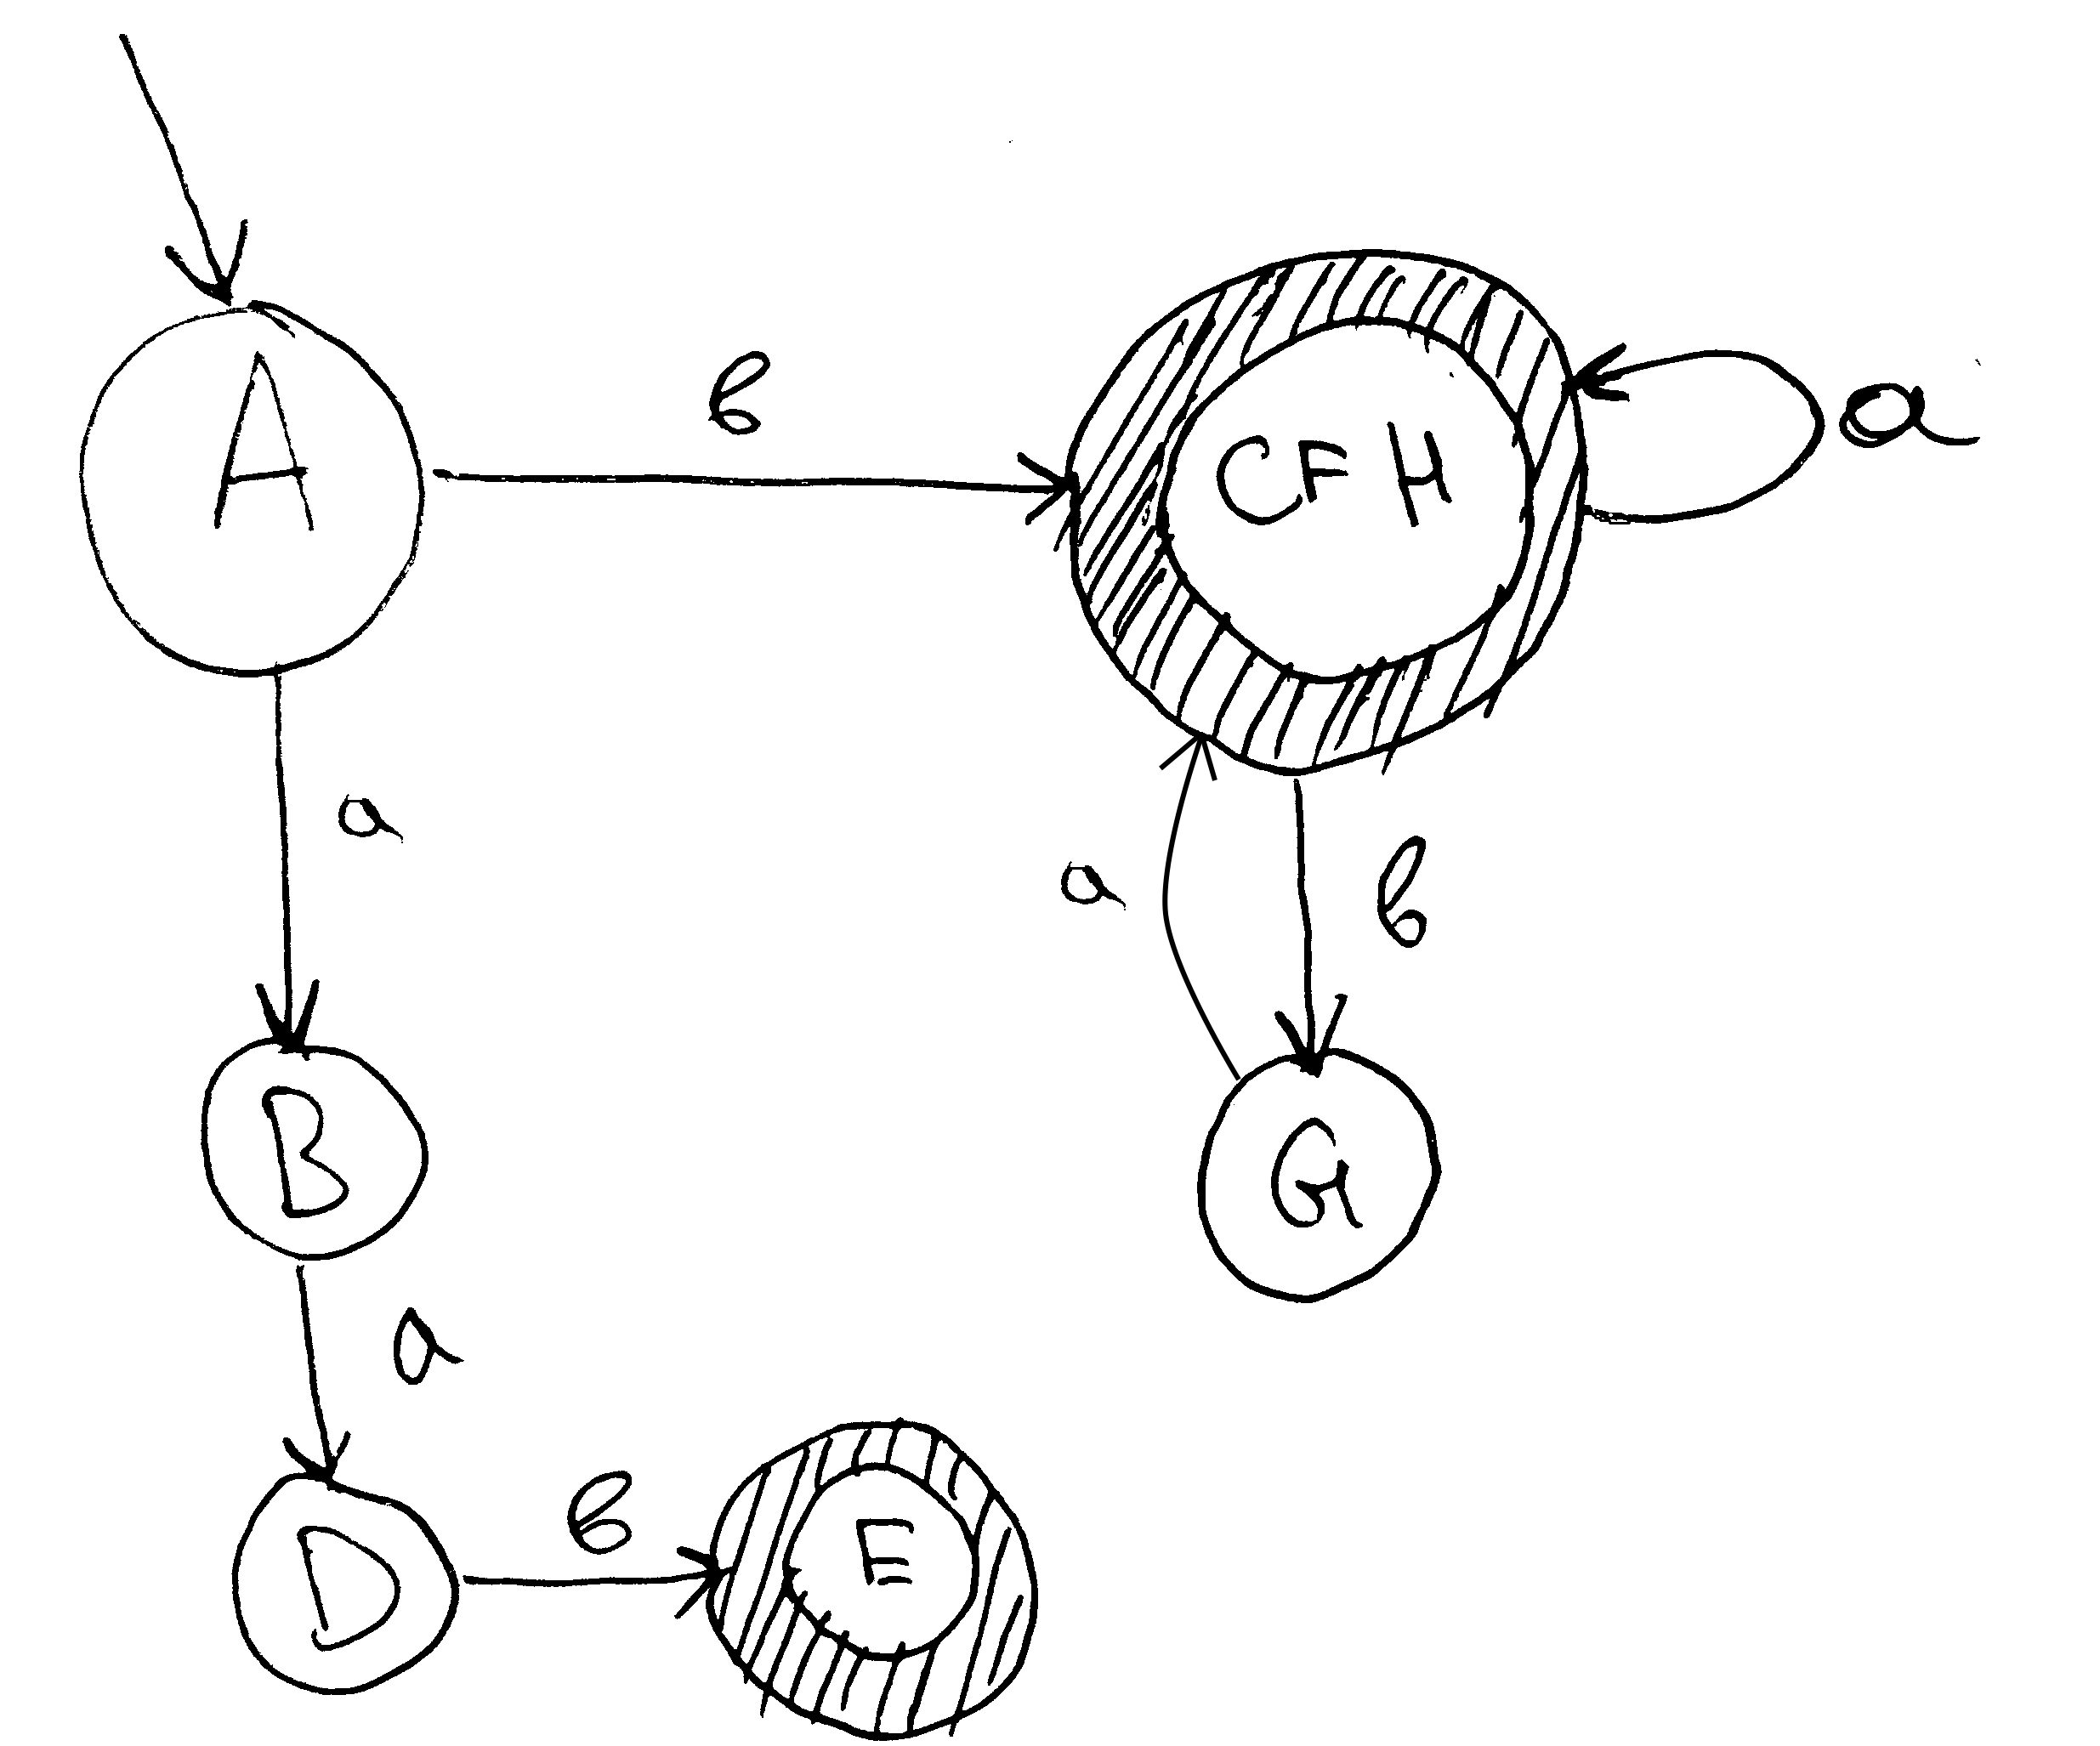
\includegraphics[scale=0.13]{data/pic4_2.png}
	\newpage
	\section{Почему это работает}
	На мой взгляд сам алгоритм говорит сам за себя, но чуть громче он будет говорить на фоне вот
	такого автомата:\\\\
	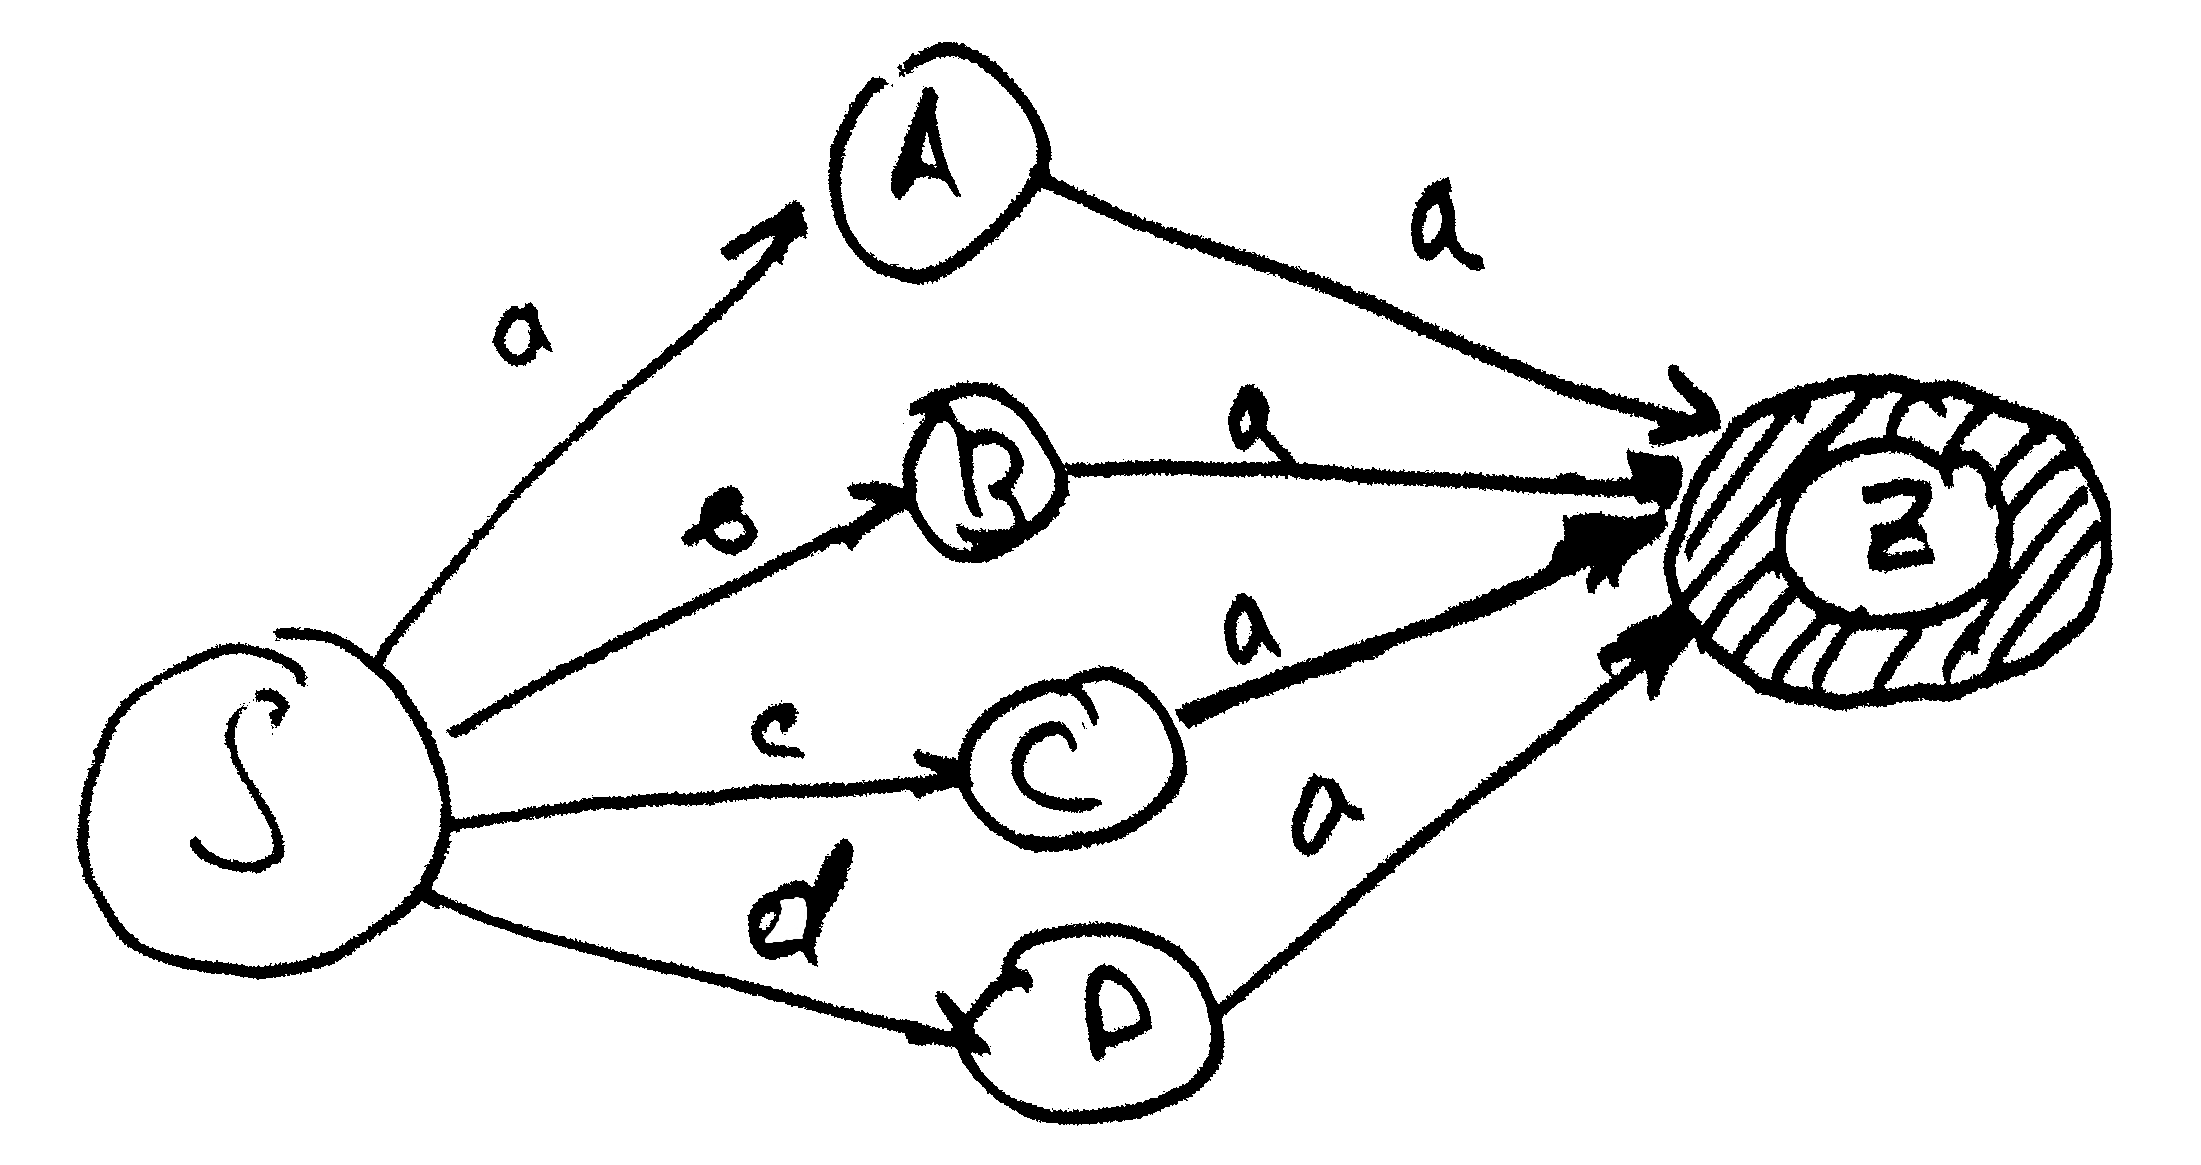
\includegraphics[scale=0.14]{data/pic4_3.png}
	\newpage
	\chapter{Отрицание, пересечение и объединение автоматов}
	Отрицание автомата $AVT$ - такой автомат $\overline{AVT}$, который успешно обрабатывает
	любую цепочку, которую не обрабатывает $AVT$.\\\\
	Пересечение автоматов $AVT1$ и $AVT2$ - такой автомат $AVT3$, который успешно обрабатывает
	любую цепочку, которую успешно обрабатывает и $AVT1$, и $AVT2$.\\\\
	Объединение автоматов $AVT1$ и $AVT2$ - такой автомат $AVT3$, который успешно обрабатывает
	любую цепочку, которую успешно обрабатывает хотя бы один из $AVT1$, $AVT2$.\\\\
	Любопытный читатель может спросить: а на кой это вообще все надо?\\
	Ну во-первых, такое задание могут дать на экзамене.\\
	А во-вторых, такое задание могут дать на экзамене в скрытой форме: вас могут попросить
	построить автомат, который принимает слова данной грамматики, но только четной длины.\\
	Тогда можно построить 2 автомата: первый принимает слова данной грамматики, а второй - слова
	четной длины. После этого их можно пересечь и радоваться жизни.
	\section{Алгоритм}
	Все алгоритмы требуют, чтобы автоматы были полные. Поэтому если надо, дополняем их.\\
	\section{Отрицание}
	Тут все предельно просто - взяли полный автомат, в нем все состояния, которые не были
	конечными, сделали конечными. А все состояния, которые были конечными, сделали неконечными.\\
	...\\
	Ну вот в принципе и все.\\
	Вот живой пример:\\
	Взяли автомат\\
	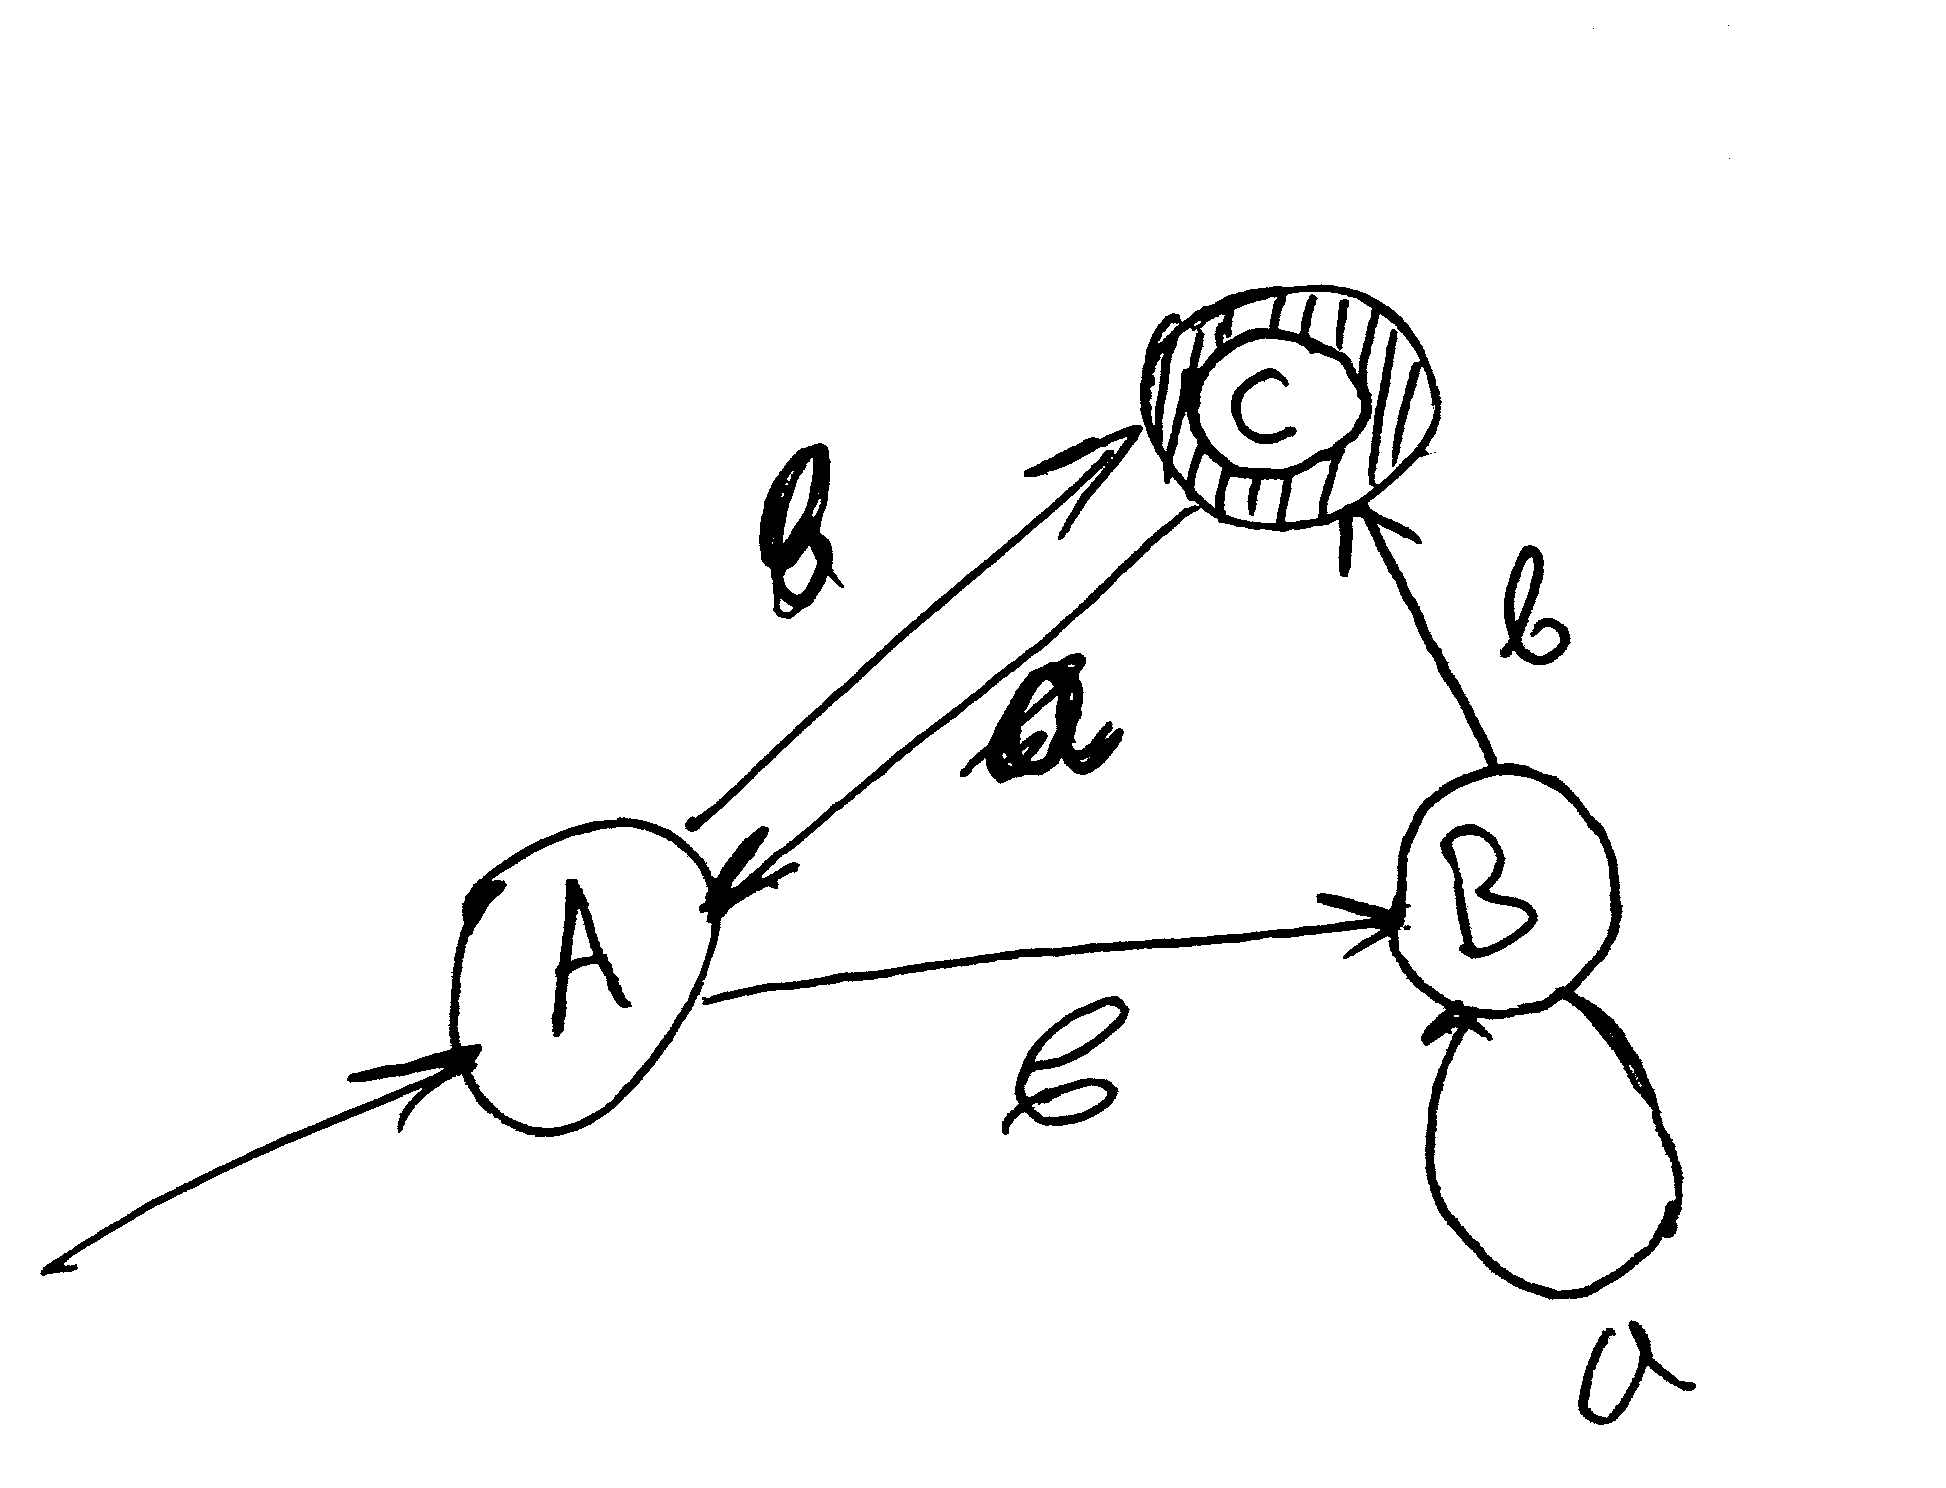
\includegraphics[scale=0.1]{data/pic5_1.png}\\
	Дополнили и проотрицали\\
	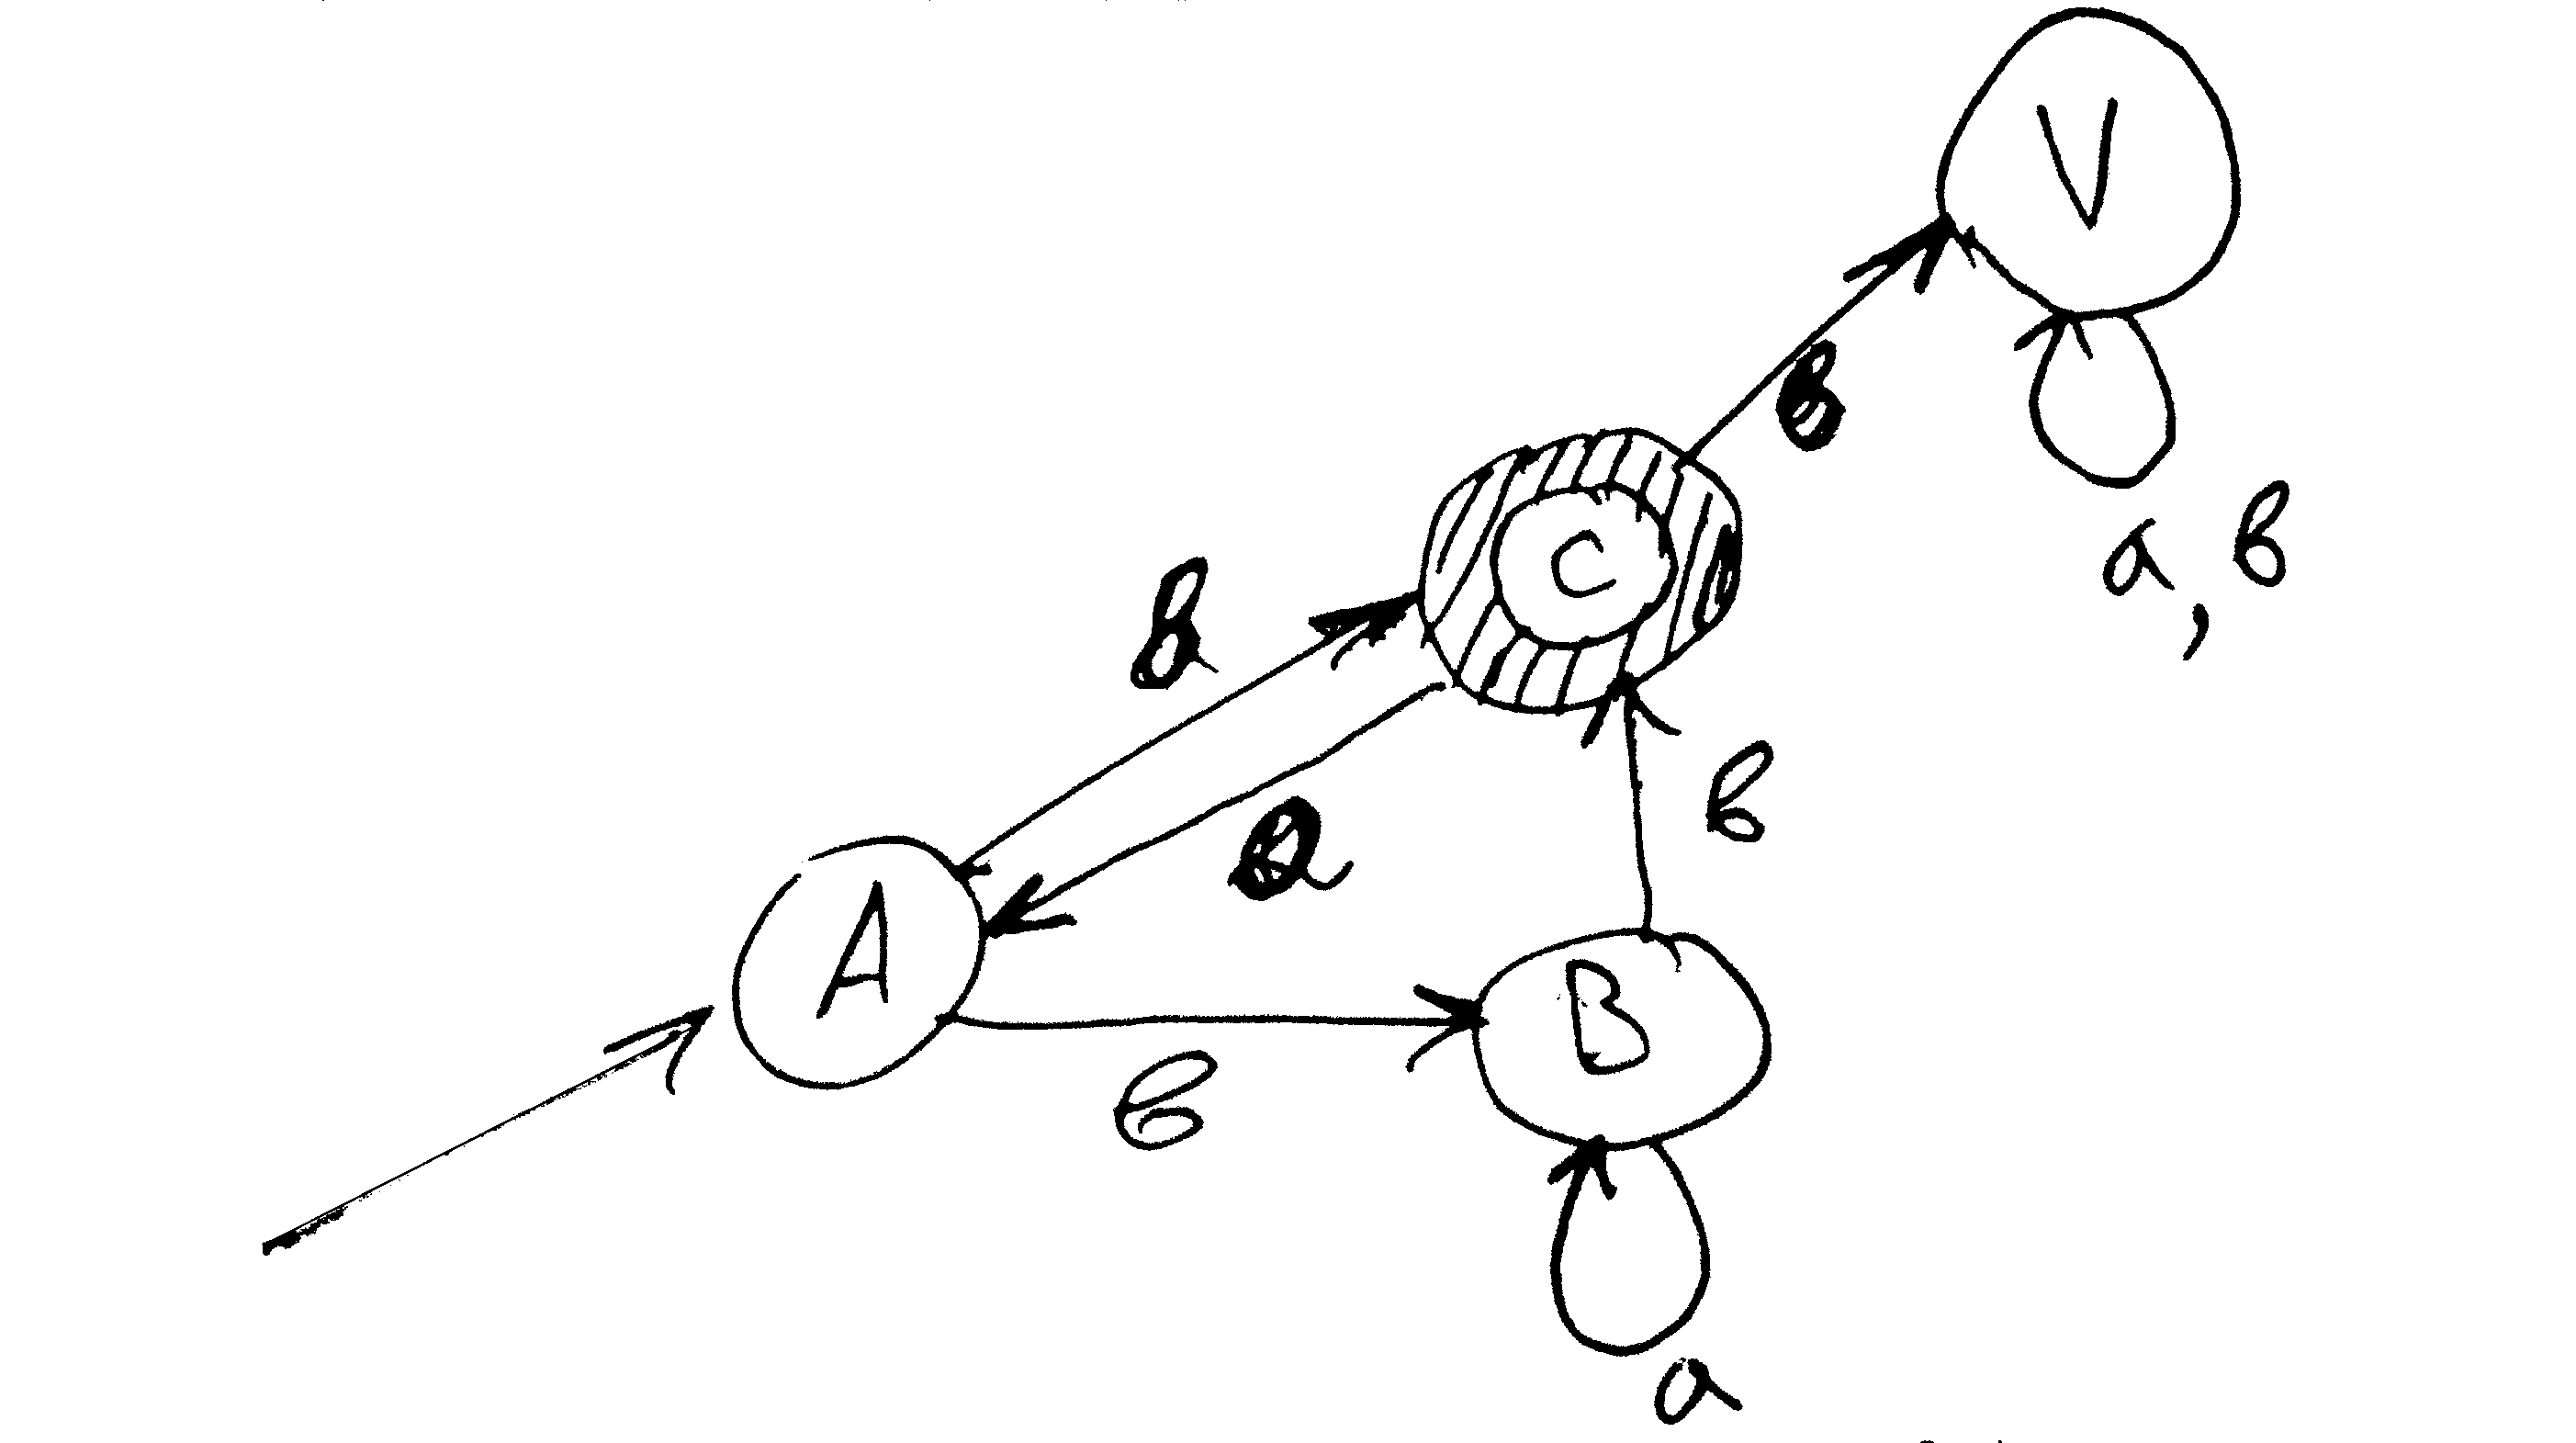
\includegraphics[scale=0.1]{data/pic5_2.png}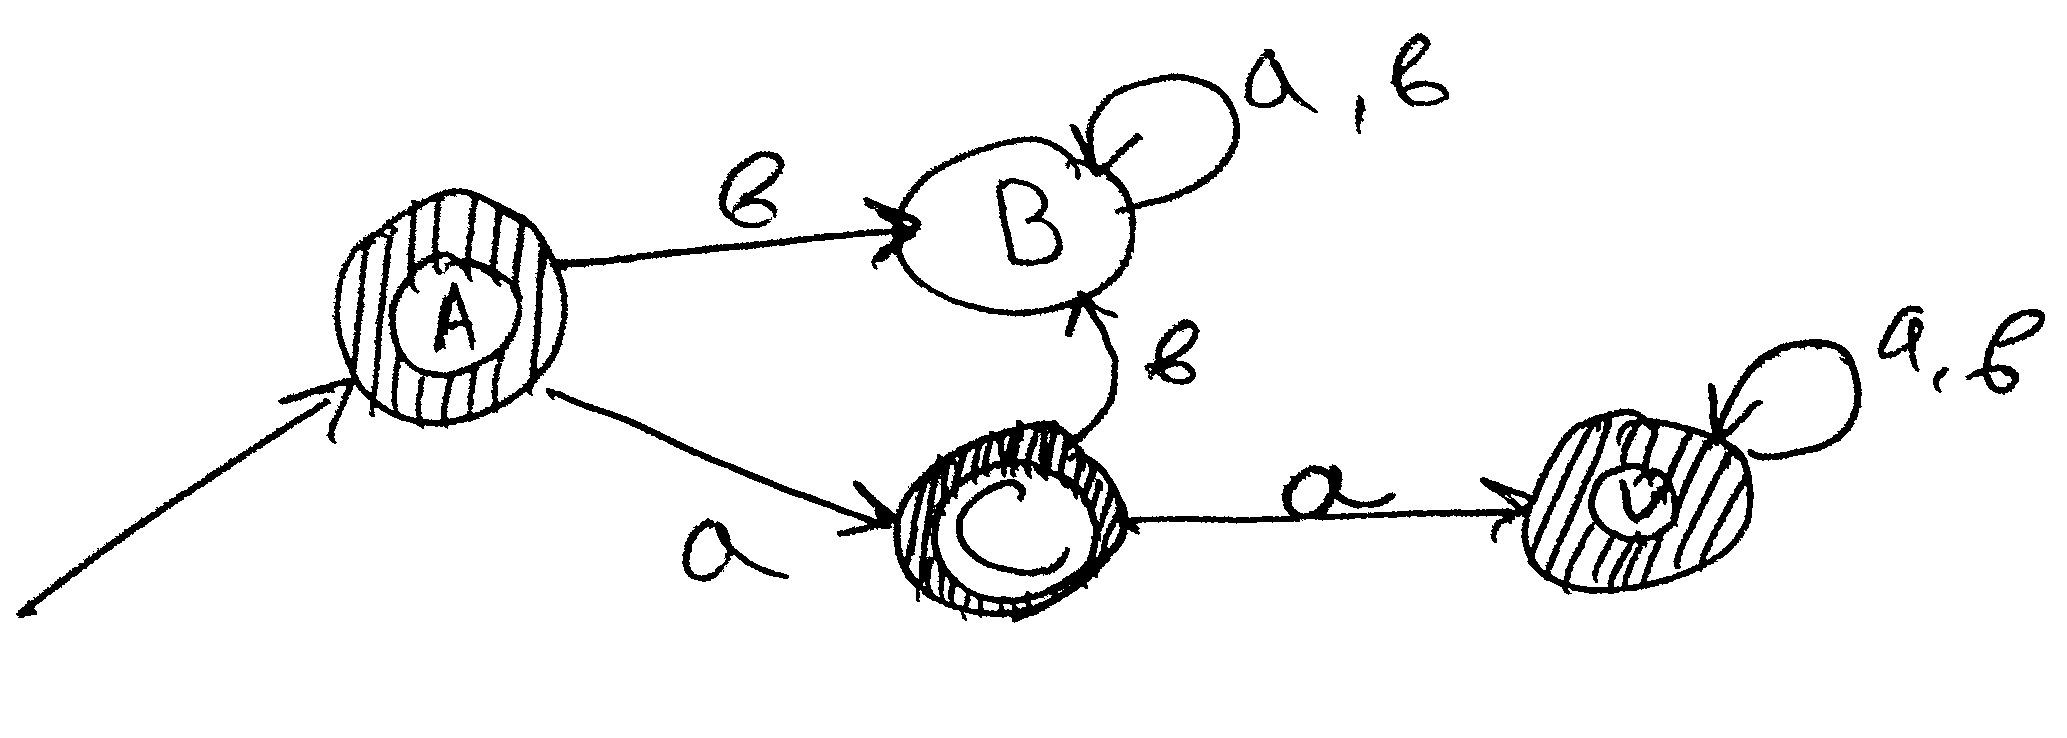
\includegraphics[scale=0.12]{data/pic5_3.png}\\
	\section{Почему это работает}
	Очевидно, что если цепочка принадлежит исходному языку, то автомат остановится в своем
	конечном состоянии. А если цепочка не принадлежит - в любом другом состоянии. Поэтому мы
	просто берем и меняем местами конечные и неконечные состояния. При этом полнота автомата
	необходима - ведь иначе мы потеряем часть слов, которые изначально не принадлежали старому
	языку, но принадлежат новому.
	\section{Пересечени и объединение}
	Здесь мы возьмем 2 следующих автомата:\\
	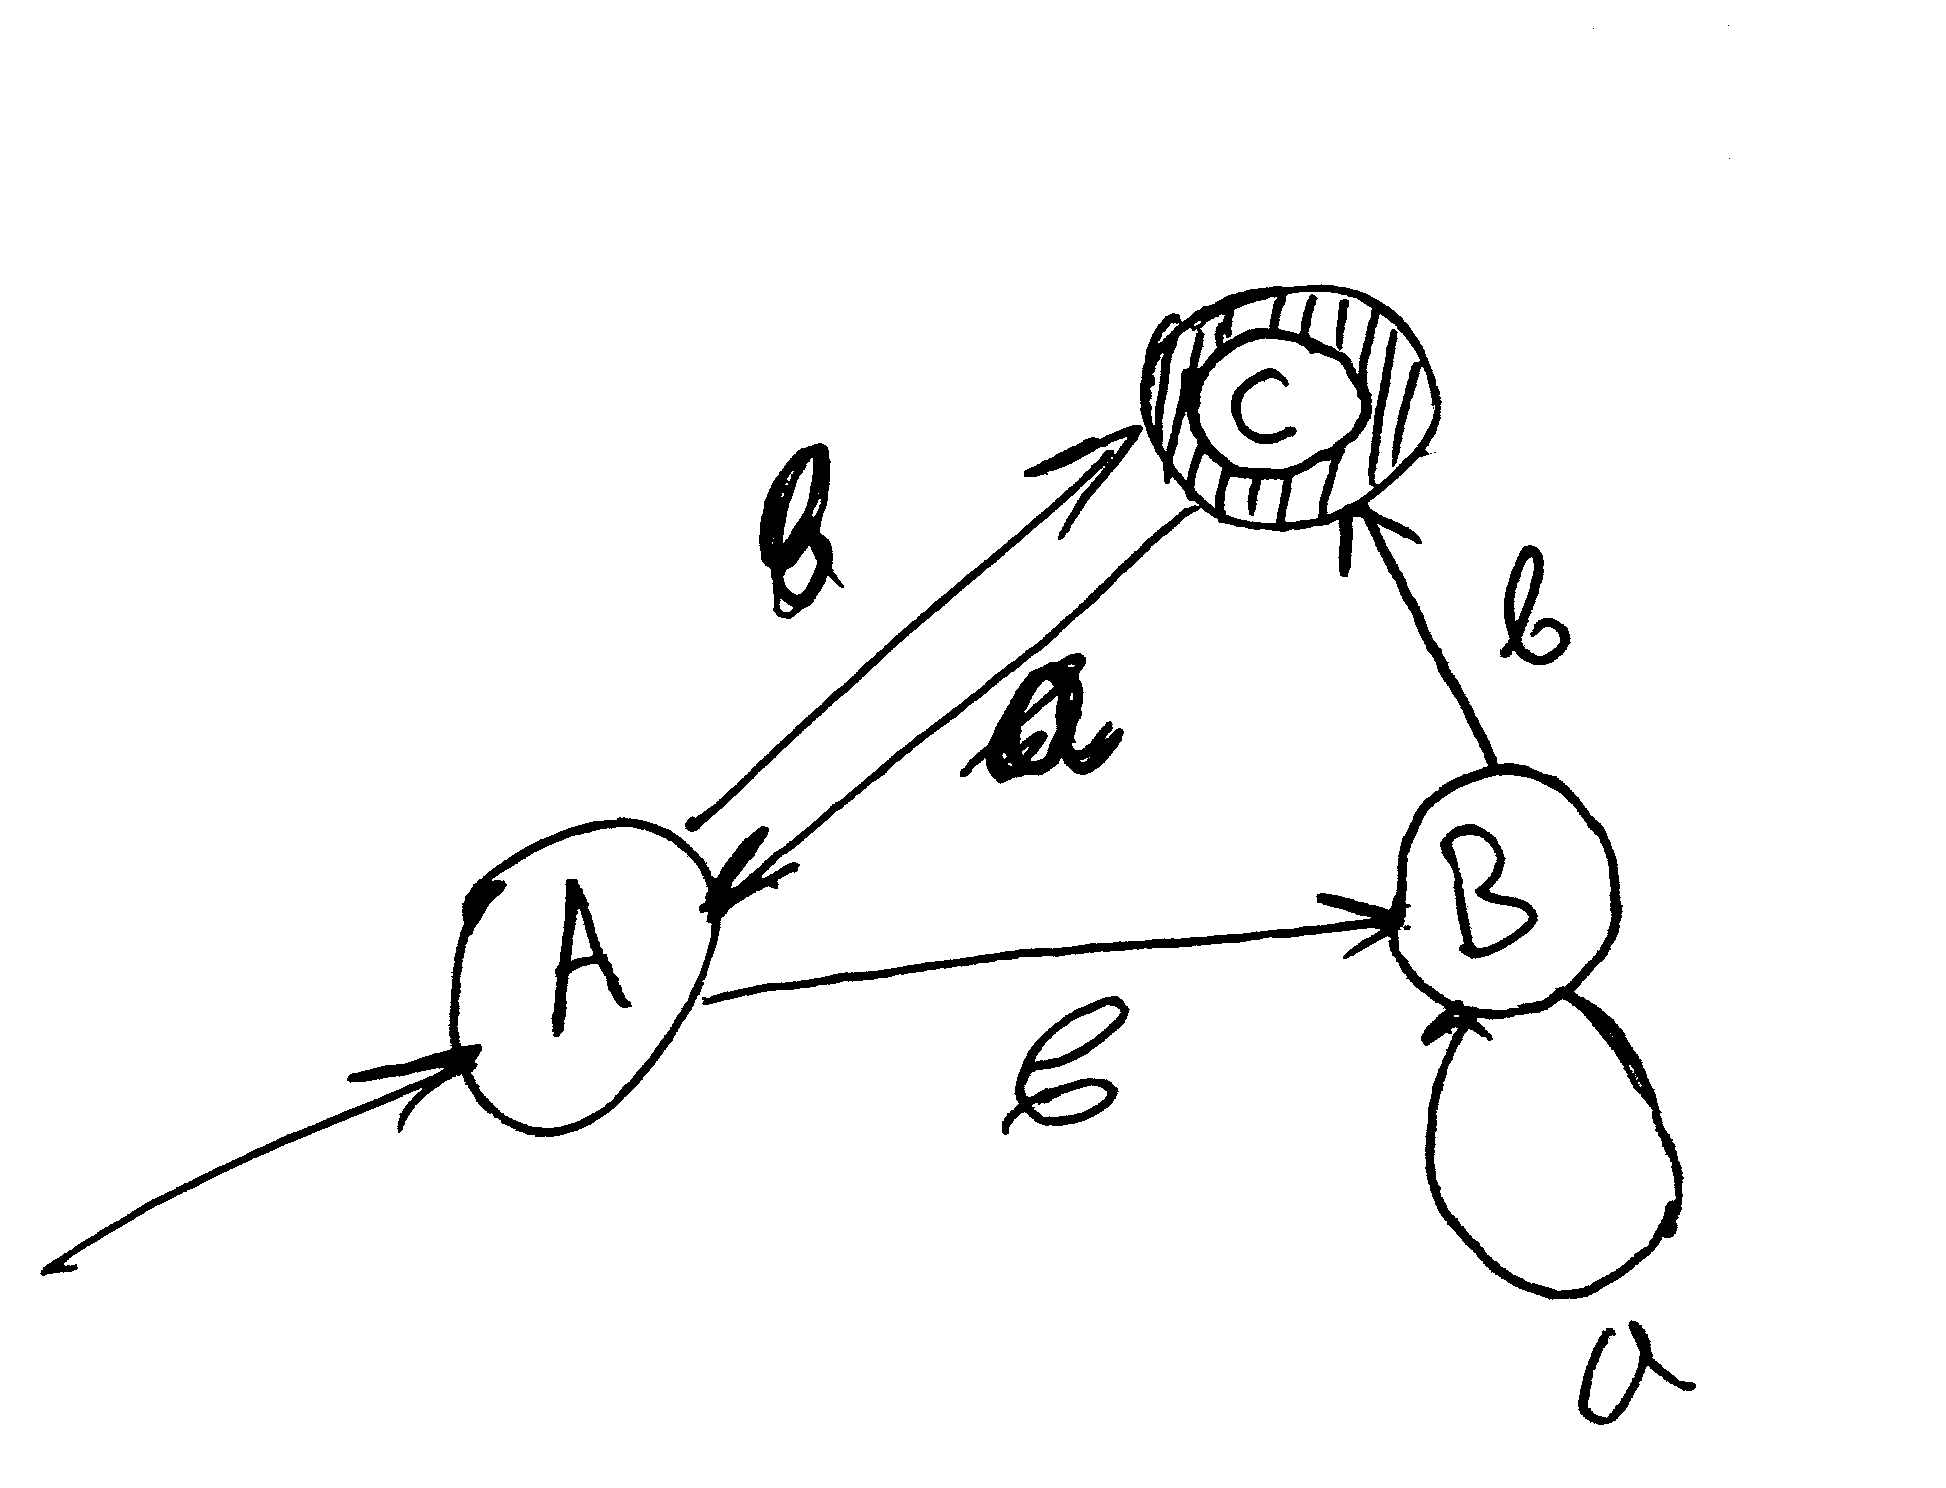
\includegraphics[scale=0.11]{data/pic5_1.png}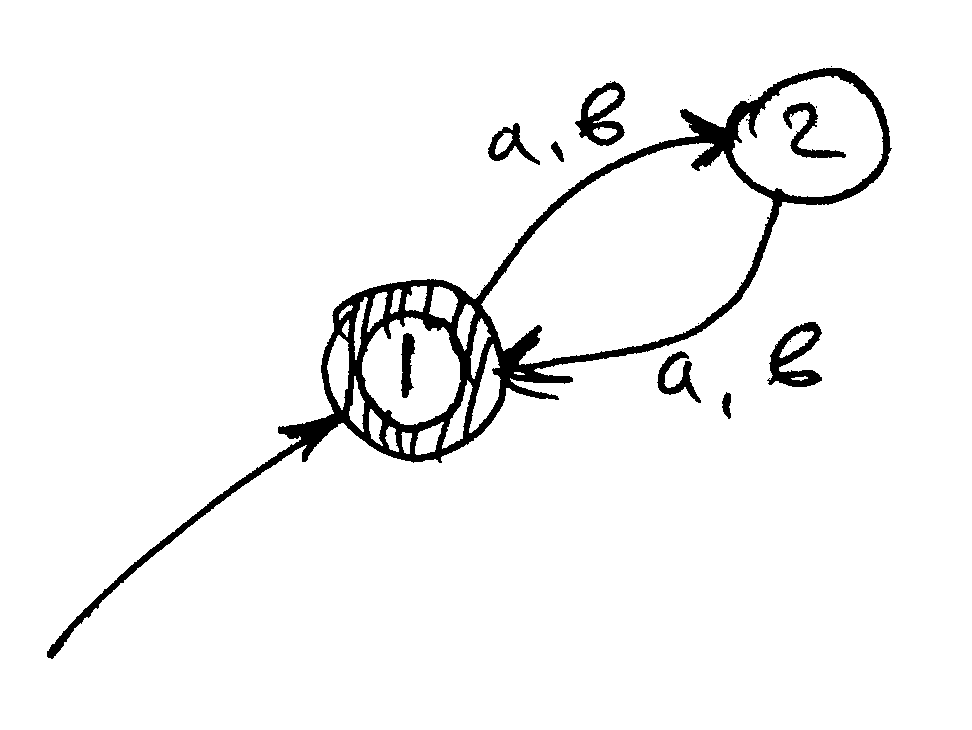
\includegraphics[scale=0.11]{data/pic5_4.png}\\
	Возьмем их дополненные версии:\\
	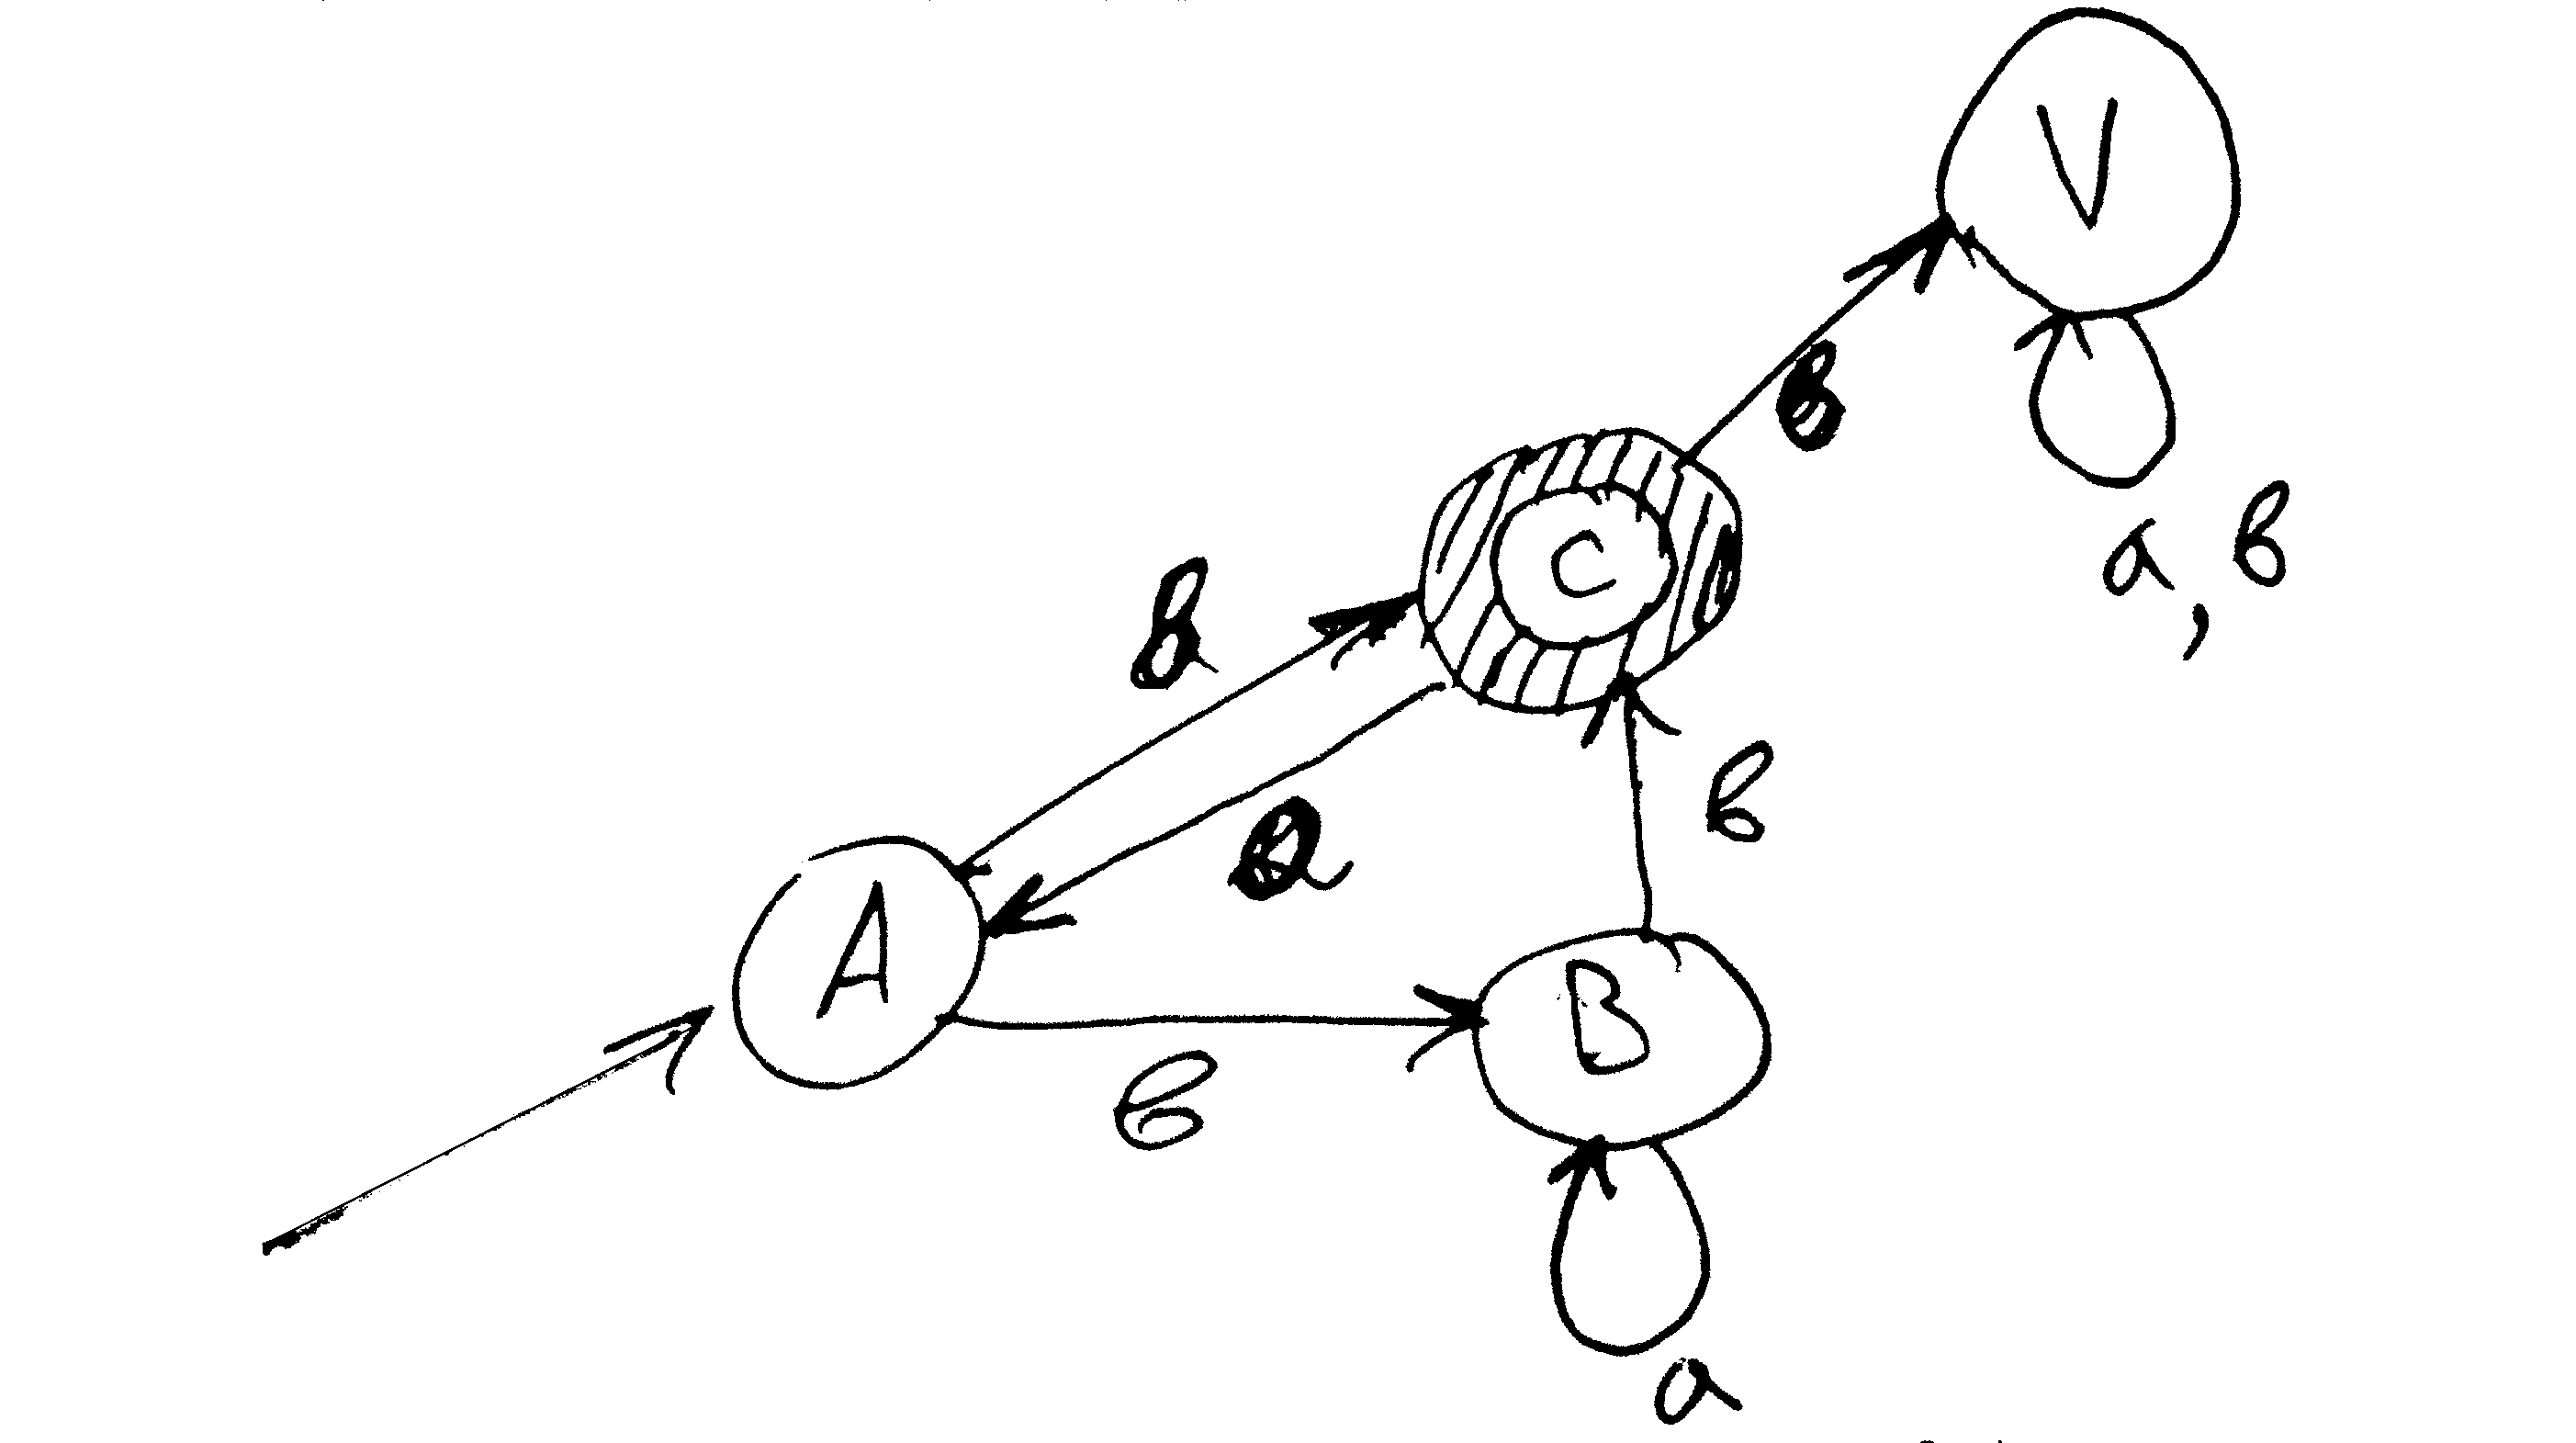
\includegraphics[scale=0.1]{data/pic5_2.png}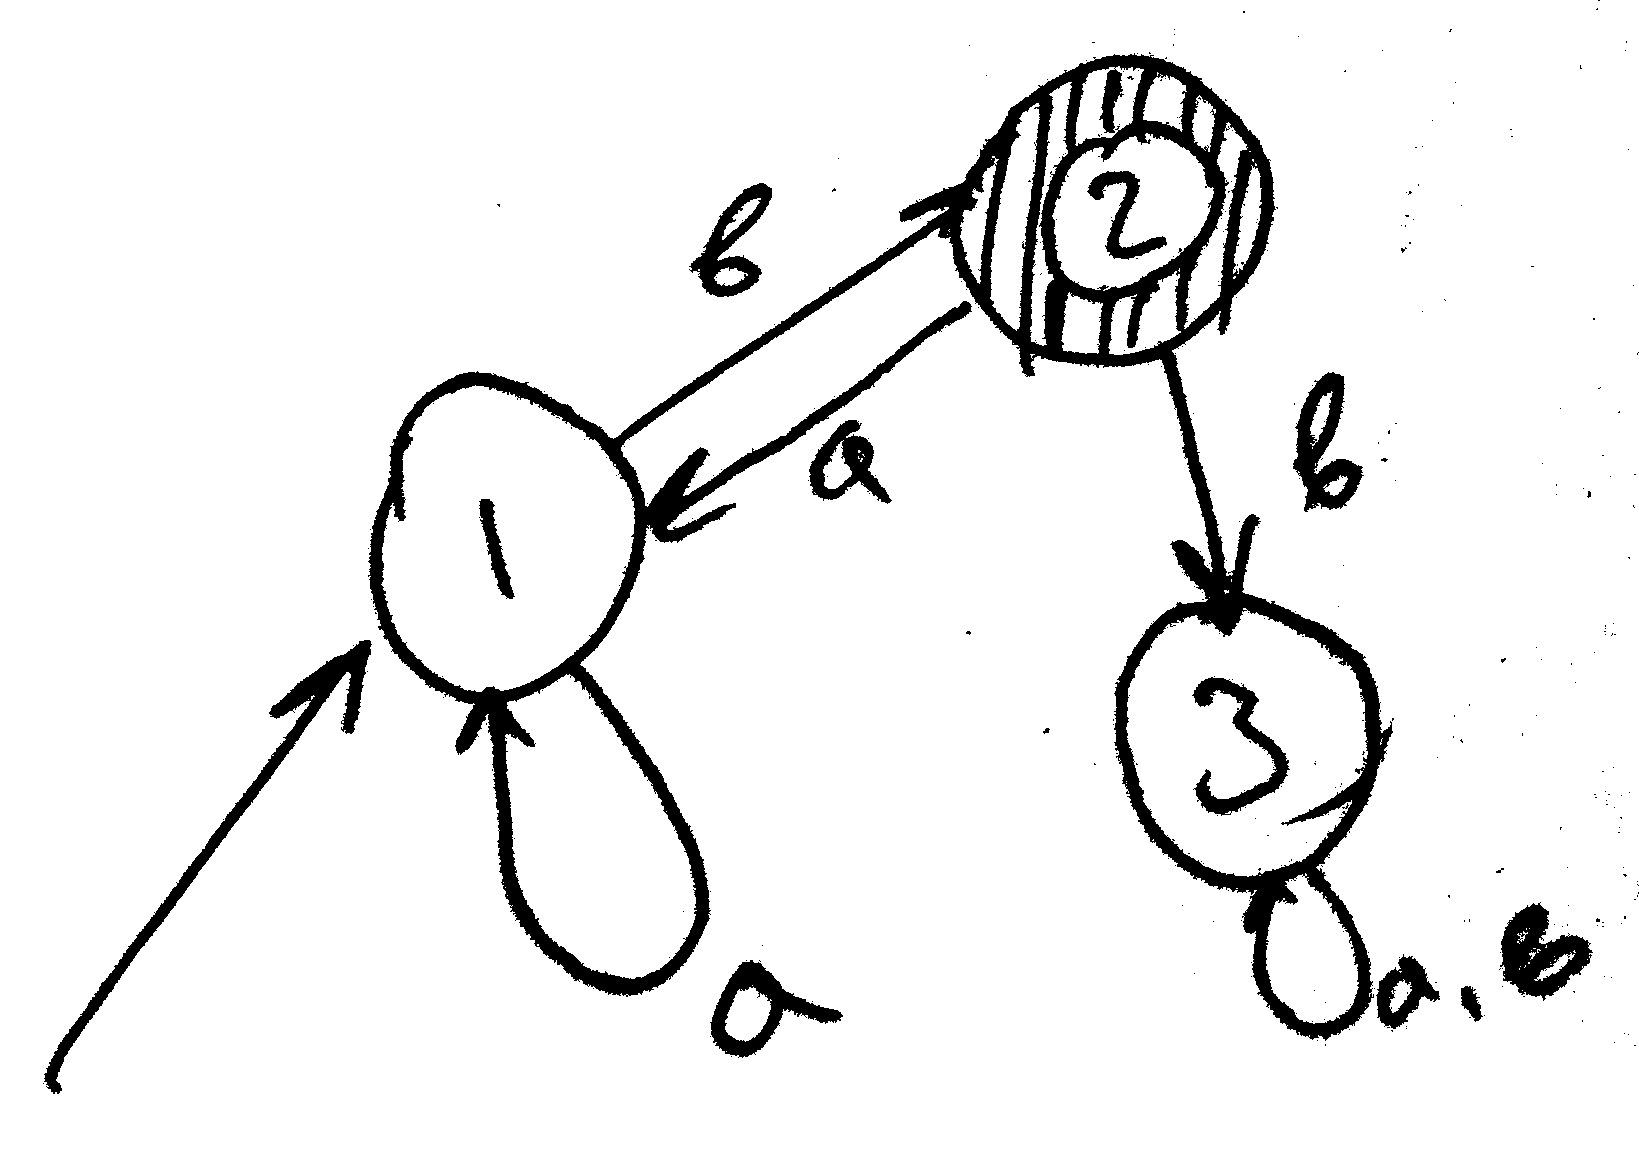
\includegraphics[scale=0.1]{data/pic5_5.png}\\
	Теперь все будет немножко сложнее. Для начала нужно построить прямое произведение
	двух автоматов.\\\\
	Можно было бы привести "очень математическое" определение прямого произведения, но оно
	хоть и очень точное, но вообще не выразительное, поэтому будем объяснять на словах.\\\\
	Прямое произведение автоматов очень понятно смотрится на фоне перемещения в двухмерном
	пространстве (ну или в n-мерном, если мы пересекаем n автоматов, но тут я могу понадеяться,
	что моему бедному читателю никогда не придется делать произведение больше 2х автоматов).\\
	Очень удобно представлять, что первый автомат символизирует собой перемещение по оси $OX$,
	а второй - по $OY$. Начальное состояние - точка $(A, 1)$. По символу $b$ по $OX$ мы переходим
	в точку $C$, а по $OY$ - в 2. В итоге мы находимся в точке $(C, 2)$. По символу $a$ по $OX$
	мы переходим обратно в $A$, а по $OY$ - обратно в $1$. Дальше, допустим, нам прилетает 
	символ $a$. По $OX$ мы переносимся в точку $B$, а по $OY$ остаемся в 1. А потом нам, например,
	прилетает символ и по $OX$ мы переносимся в $C$, а по $OY$ - в 2.\\
	На рисунке изображены символические перемещения в двухмерном пространстве.\\
	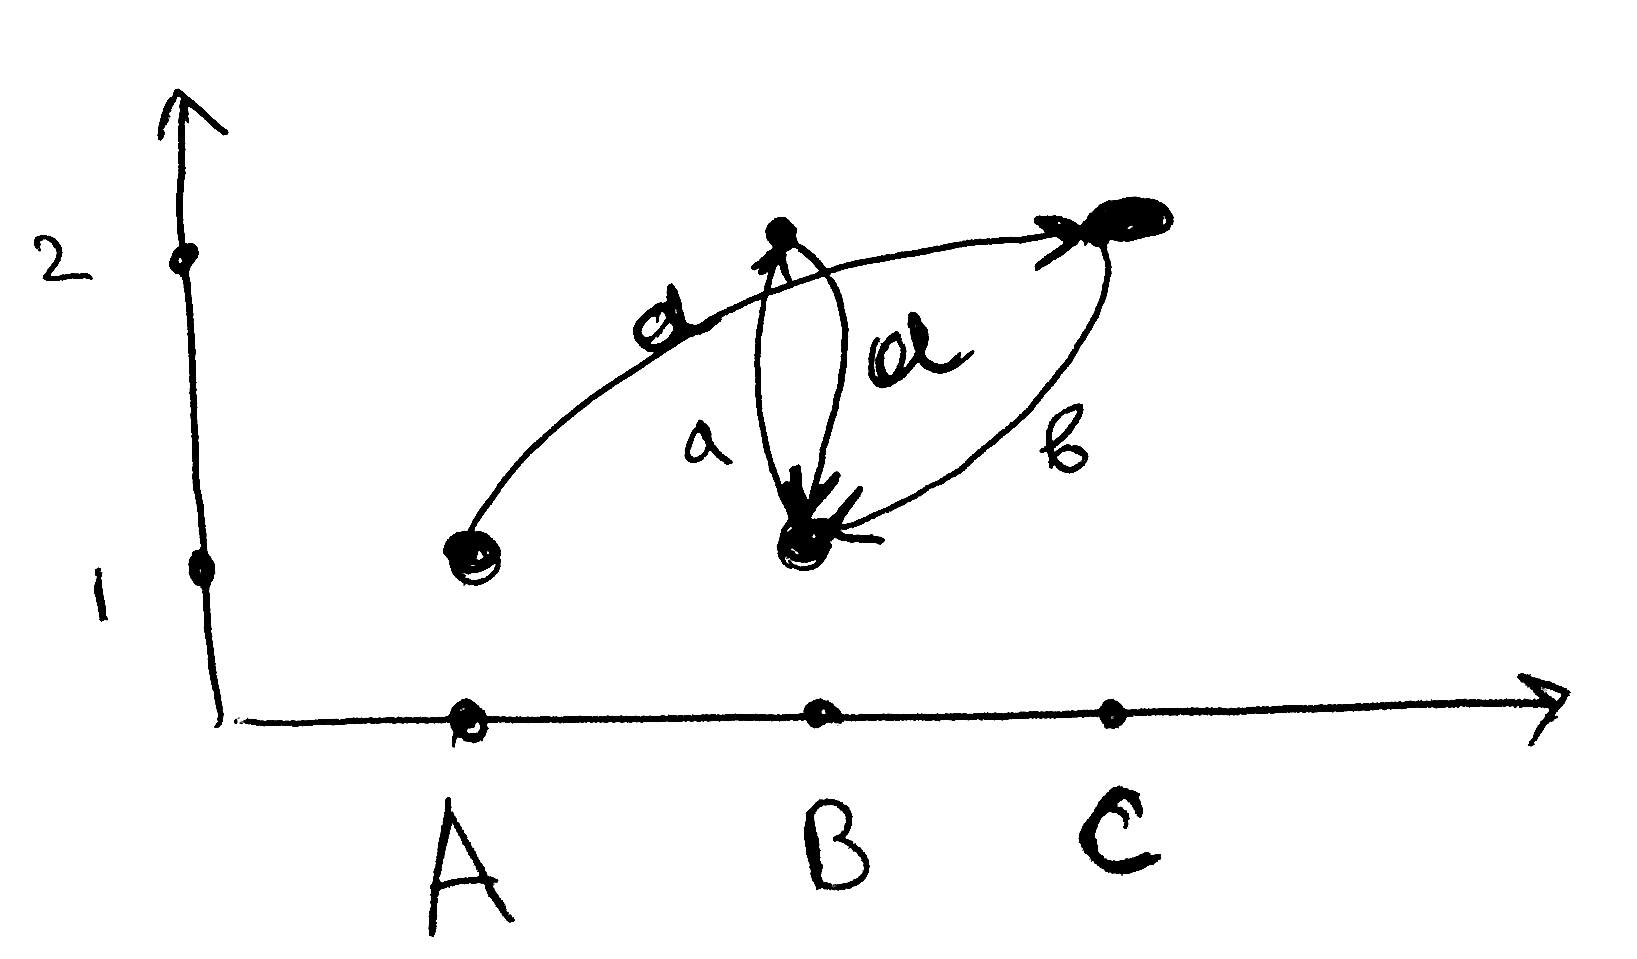
\includegraphics[scale=0.14]{data/pic5_6.png}\\
	Внимательный читатель мог заметить, что все эти перемещения напрямую связаны с автоматами,
	которые мы обрабатываем. По сути мы пытаемся усидеть на двух стульях, перемещаясь одновременно
	по двум автоматам.\\
	И тут приходит в голову мысль: зачем нам постоянно помнить, что в первом
	автомате мы находимся в состоянии $S$, а во втором - в состоянии $Q$, если можно просто
	сделать вид, что автомат на самом деле один, а мы находимся в состоянии $SQ$. Если в первом
	автомате мы по символу $a$ переходим в состояние $P$, а во втором - в состояние $R$, то мы
	просто вспоминаем, что автомат на самом деле один, а мы просто из $SQ$ по $a$ переходим в
	$PR$.\\
	Давайте же построим произведение наших полных автоматов:\\
	Это куда удобнее делать с помощью таблицы. Для начала нужно сделать таблицу для исходных
	автоматов:\\
		\begin{tabular}{lcc}
			 & $a$ & $b$ \\
			 $A$ & $B$ & $C$ \\
			 $B$ & $B$ & $C$ \\
			 $*C$ & $A$ & $V$ \\
			 $V$ & $V$ & $V$ \\
		\end{tabular}\hspace*{80pt}
		\begin{tabular}{lrr}
			 & $\ a$ & $\ b$ \\
			 $1$ & $1$ & $2$ \\
			 $*2$ & $1$ & $3$ \\
			 $3$ & $3$ & $3$ \\
		\end{tabular}\\\\
	А теперь строим таблицу произведения (это очень скучно):\\
		\begin{tabular}{lcc}
			 & $a$ & $b$ \\
			 $A1$ & $B1$ & $C2$ \\
			 $B1$ & $B1$ & $C2$ \\
			 $C1$ & $A1$ & $V2$ \\
			 $V1$ & $V1$ & $V2$ \\
			 $A2$ & $B1$ & $C3$ \\
			 $B2$ & $B1$ & $C3$ \\
			 $C2$ & $A1$ & $V3$ \\
			 $V2$ & $V1$ & $V3$ \\
			 $A3$ & $B3$ & $C3$ \\
			 $B3$ & $B3$ & $C3$ \\
			 $C3$ & $A3$ & $V3$ \\
			 $V3$ & $V3$ & $V3$ \\
		\end{tabular}\\\\\\\\
	Это ВСЕ возможные сочетания состояний из первого и второго автомата. Но педантичный читатель
	мог заметить, что по факту нужны далеко не все (в силу того, что больше половины из них
	недостижимы). Действительно, учитывая, что начальное состояние это состояниие состоящие
	из начальных состояний двух старых автоматов, а именно $A1$, достижимы только состояния
	$A1,B1,C2,V3$.\\
	Поэтому вполне хватит такой таблицы:\\
		\begin{tabular}{lcc}
			 & $a$ & $b$ \\
			 $A1$ & $B1$ & $C2$ \\
			 $B1$ & $B1$ & $C2$ \\
			 $C2$ & $A1$ & $V3$ \\
			 $V3$ & $V3$ & $V3$ \\
		\end{tabular}\\\\
	Остается вопрос: что же взять в качестве множества конечных состояний?\\
	Вот тут уже зависит от задачи: если у нас пересечение, то мы берем состояние, состоящее
	только из конечных состояний старых автоматов (в данном случае $C2$).\\
	Если же у нас объединение, то мы берем состояния, в составе которых есть хотя бы одно
	конечное состояние (в данном случае это могли бы быть $A2, B2, C2, V2, C1, C3$, но
	пример вышел неудачный и из достижимых осталось только $C2$, а подбирать другие
	автоматы слишком лень).\\
	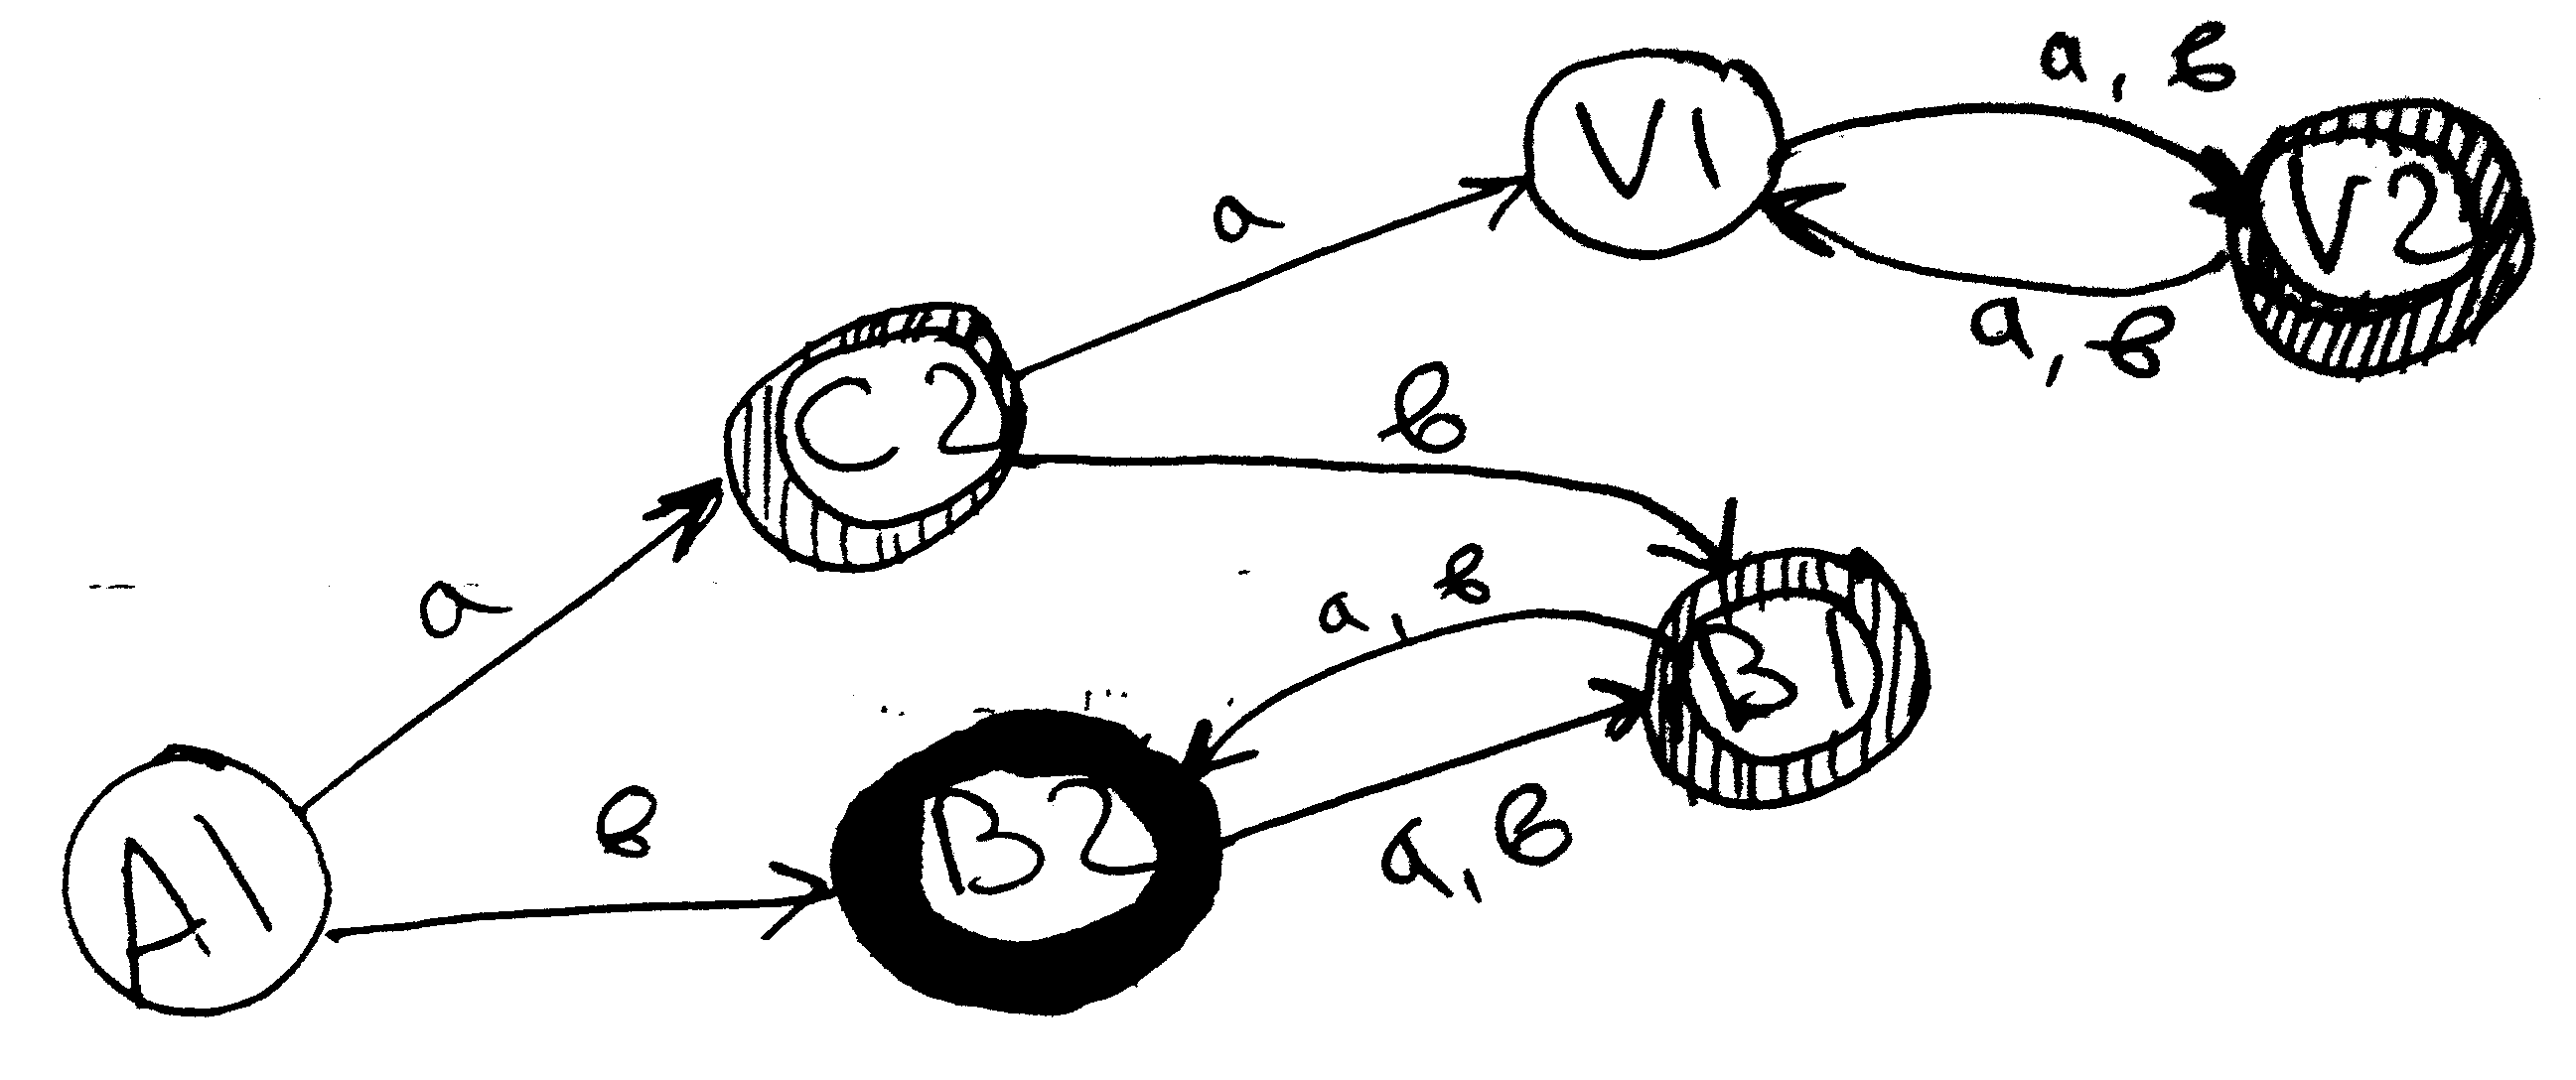
\includegraphics[scale=0.09]{data/pic5_7.png}\\
	А получилось так потому, что второй автомат является сокращенной версией
	первого, но мне все еще слишком лень что-то переделывать.\\
	\section{Почему это работает}
	Саму концепцию произведения я вроде расписал через двухмерное пространство. Почему же мы
	именно так выбираем конечные состояния в случае пересечения и произведения?\\
	Все просто: в случае пересечения нам надо, чтобы оба автомата остановились в своих конечных
	состояниях (потому что слово должно принадлежать обеим языкам). Соответсвенно, нам нужны
	состояния, состоящие из конечных состояний автоматов. Абсолютно аналогичная ситуация с
	объединением: нам нужно, чтобы хотя бы один из исходных автоматов остановился в своем
	конечном состоянии.
	
	\chapter{Построение автомата по праволинейной грамматике}
	\section{Алгоритм}
	$S$ - аксиома грамматики. Значит, начальное состояние у нас $S$. Множество конечных
	состояний $F$ описывается так: если есть переход $S \to e$, тогда $F=\{S,R\}$,
	иначе $F=\{R\}$ ($R$ это просто финальное состояние, такого терминала вообще в
	грамматике быть не должно)\\
	Переходы строятся по следующим правилам:\\
	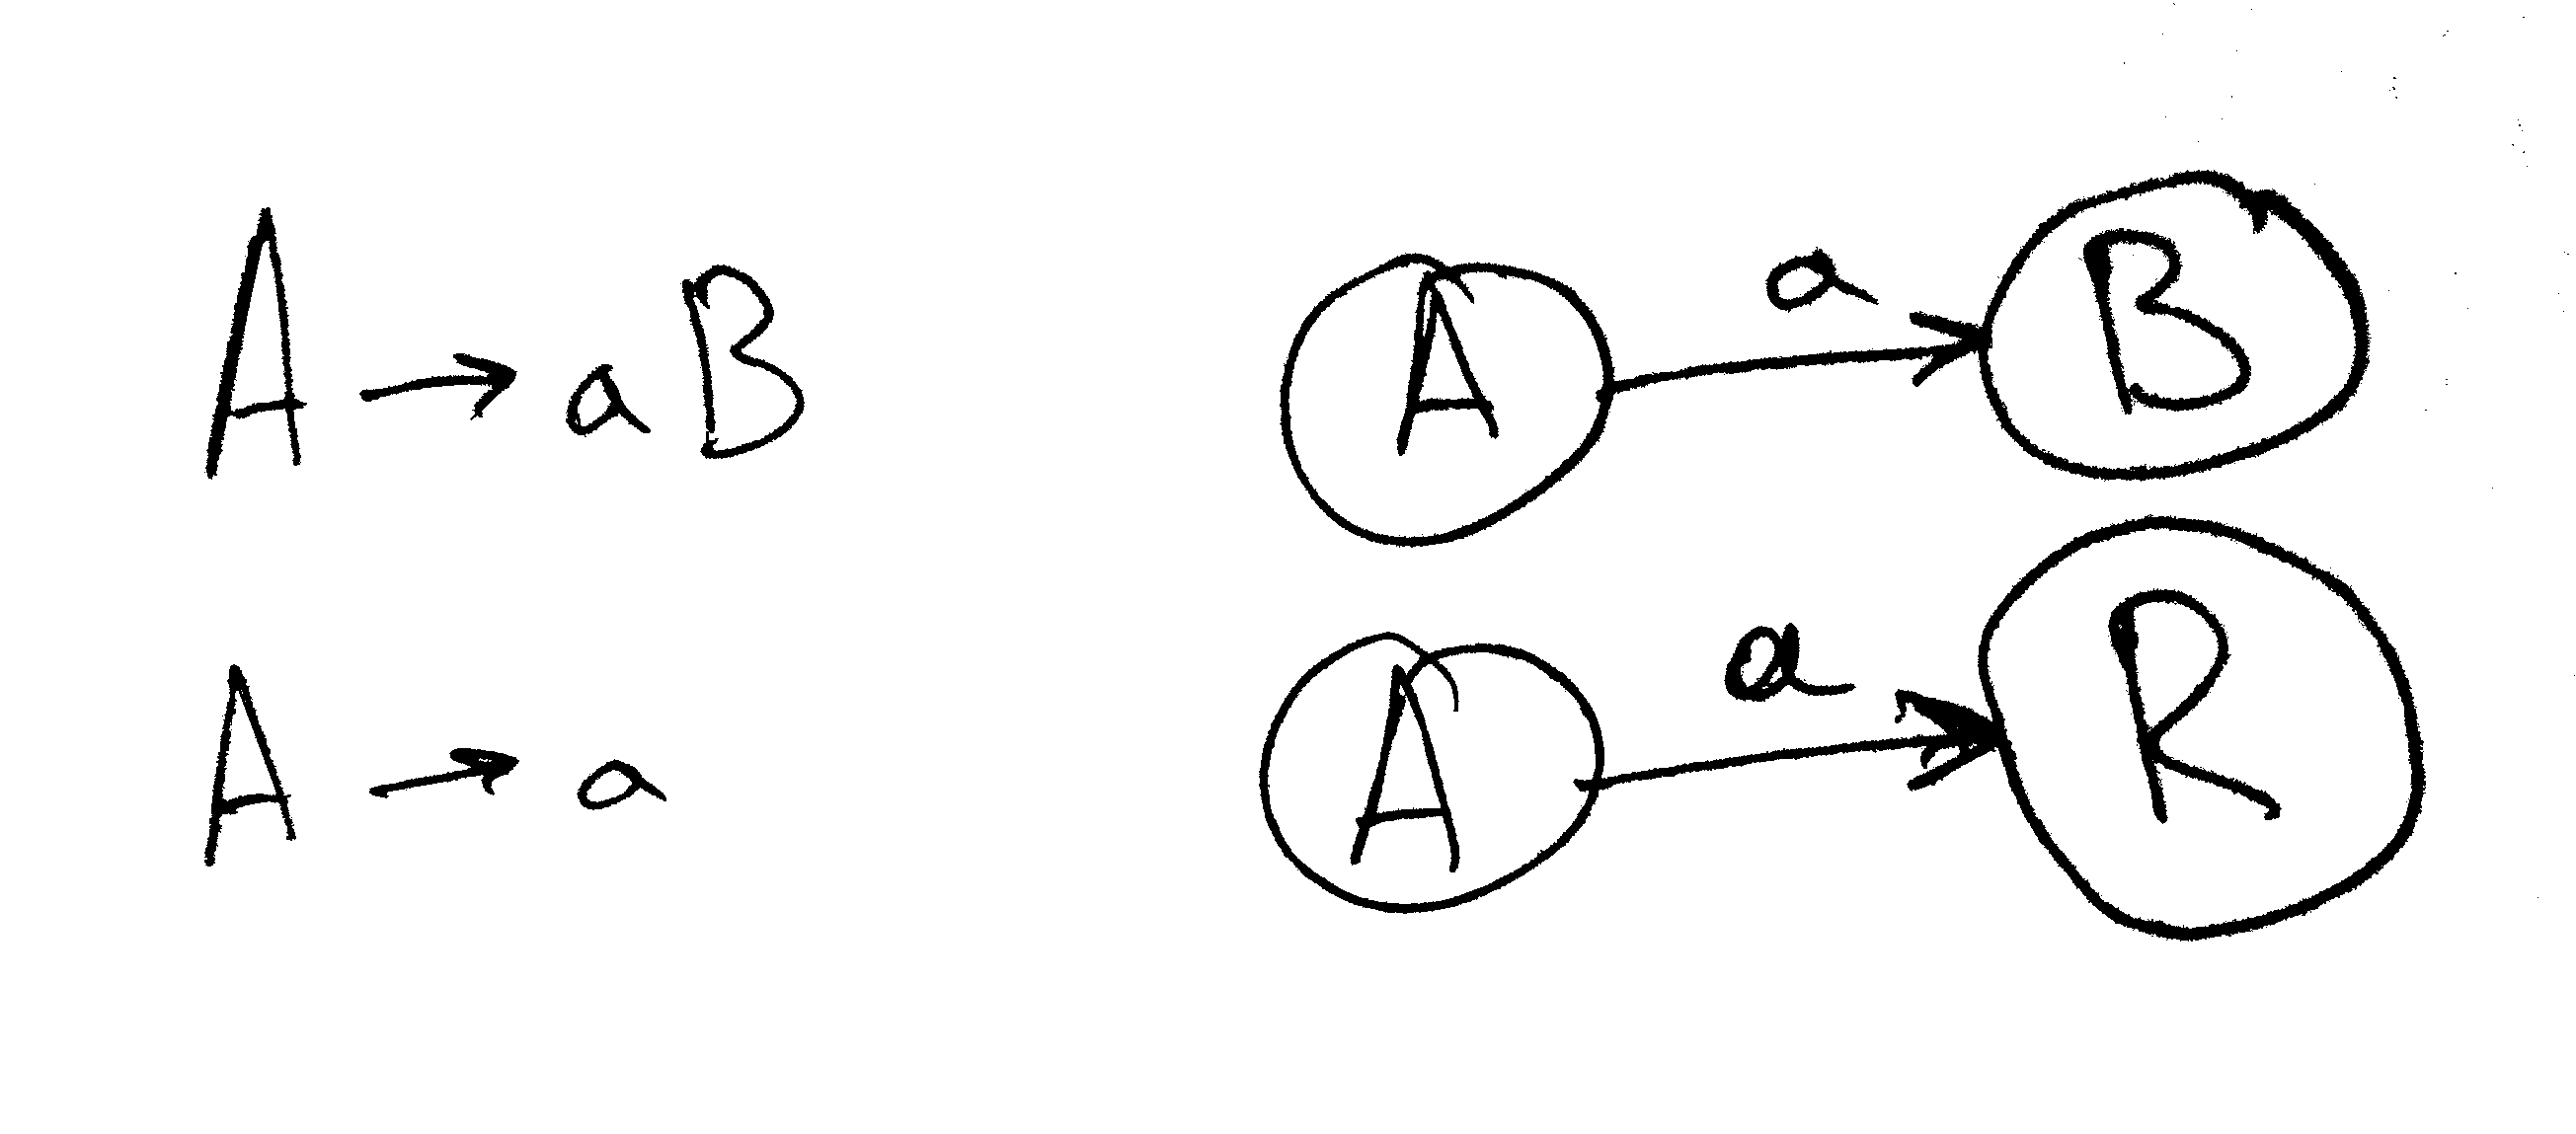
\includegraphics[scale=0.12]{data/pic6_1.png}\\
	Возьмем такую грамматику:\\
	$S \to aA | bB | c$\\
	$A \to aA | bB | cC $\\
	$B \to bB | a | c $\\
	$C \to aB | bC | cA $\\
	\newpage
	Построим автомат по правилам выше:\\
	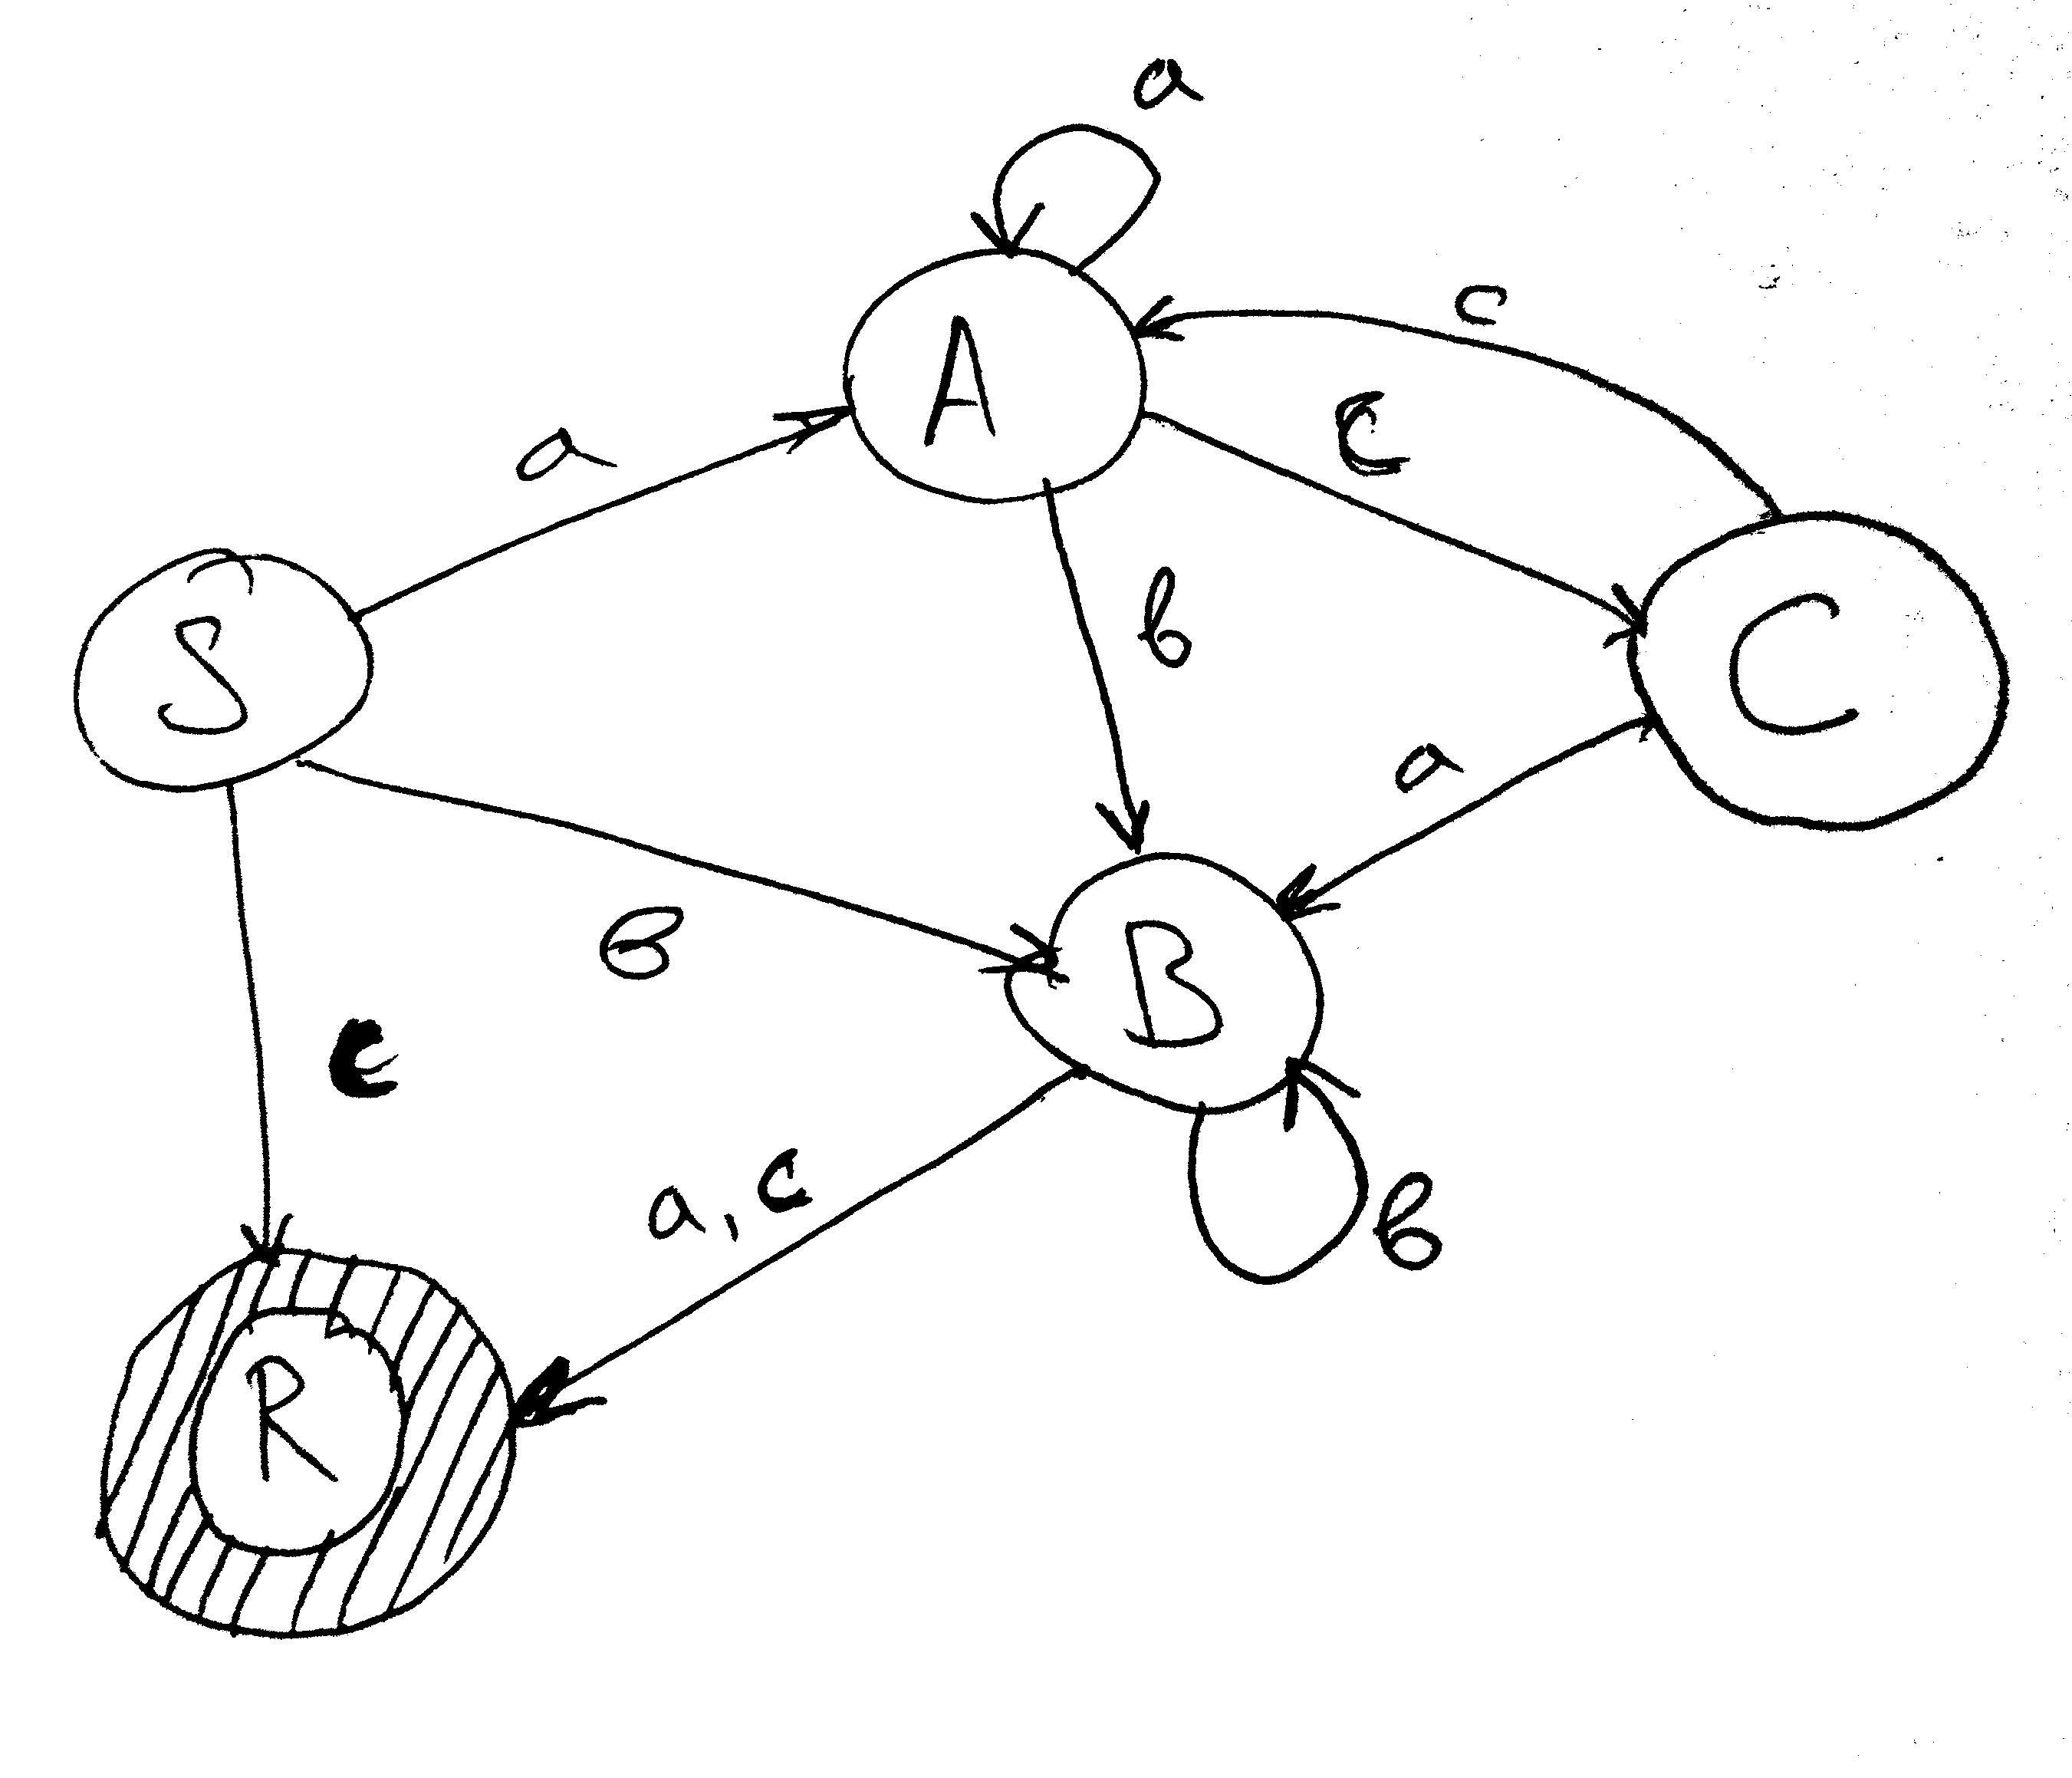
\includegraphics[scale=0.12]{data/pic6_2.png}\\
	И что, все?\\
	Ну да, все\\
	\section{Почему это работает}
	Праволинейные грамматики очень хороши хотя бы тем, что если раскручивать их, начиная
	с аксиомы $S$, мы ни в какой момент времени не сможем иметь больше одного
	необработанного нетерминала.\\
	Очень похоже на автомат: там мы тоже всегда находимся в одном состоянии (если
	автомат один).\\
	При этом правила вида $S \to aA$ говорят как бы следующее: мы разобрались с нетерминалом
	$S$, потому что увидели терминал $a$ и все для себя поняли, теперь надо 
	разобраться с нетерминалом $A$.\\
	Это уже самый натуральный автомат, где состояние $A$ соответствуте нетерминалу $A$, который
	мы еще не успели раскрутить.
	
	
	\chapter{Приведение КС-грамматики}
	\section{Алгоритм удаления бесплодных символов}
	Бесплодные символы - те, из которых невозможно вывести цепочку.\\
	Алгоритм простой:\\
	Строим множества\\
	$N_0=\{\}$\\
	$N_i=\{A; A \to a, a \in N_{i-1} \cup T^*\} \cup N_{i-1}$\\
	То есть, мы последовательно добавляем в новое множество то, из чего можно было
	бы вывести предыдущее. Все это надо повторять до стаблилзации.\\
	Рассмотри на примере:\\
	$S \to ABD | cAC $\\
	$A \to a | C $\\
	$B \to AB | BA | BD $\\
	$C \to bC | aC | cA $\\
	$D \to a | bB | c$\\\\
	$N_0=\{\}$\\
	$N_1=\{A,D\}, (A \to a, D \to a | c)$\\
	$N_2=\{A,C,D\}, (C \to cA)$\\
	$N_3=\{A,C,D,S\}, (S \to cAC)$\\
	$N_4=N_3$\\\\
	После этого нужно удалить все правила, которые были связаны с бесплодными символами.\\
	$S \to \xcancel{ABD} | cAC $\\
	$A \to a | C $\\
	$\xcancel{B \to AB | BA | BD }$\\
	$C \to bC | aC | cA $\\
	$D \to a | \xcancel{bB} | c$\\\\
	\section{Почему это работает}
	В данном случае мы просто идем с конца и смотрим, из чего мы могли бы вывести слово,
	состоящее только из терминальных символов. В конце остается множество тех нетерминалов,
	из которых можно вывести что-то годное. Соответственно, другие нам не нужны.
	\section{Алгоритм удаления недостижимых символов}
	Сразу скажу, что этот алгоритм есть смысл применять только после удаления бесплодных
	символов, потому что после этого алгоритма новые бесплодные символы появиться не
	могут, а после предыдущего новые недостижимые - легко.\\
	Алгоритм простой:\\
	Строим множества\\
	$V_0=\{S\}$\\
	$V_i=\{B; A \to aBb, A \in V_{i-1}, x,y \in T^*\} \cup V_{i-1}$\\
	То есть, мы последовательно добавляем в новое множество те нетерминалы, которые
	можно с помощью правил грамматики получить из предыдущего. Повторять до стабилизации.\\
	Рассмотрим на примере, оставшегося после работы предыдущего алгоритма:\\
	$S \to cAC $\\
	$A \to a | C $\\
	$C \to bC | aC | cA $\\
	$D \to a | c$\\\\
	$V_0=\{S\}$\\
	$V_1=\{S, A, C\}, (S \to cAC)$\\
	$V_2=V_1$\\\\
	Получили множество достижимых символов, осталось удалить все правила, связанные с
	недостижимыми.\\
	$S \to cAC $\\
	$A \to a | C $\\
	$C \to bC | aC | cA $\\
	$\xcancel{D \to a | c}$\\\\
	\section{Почему это работает}
	Если в предыдущем алгоритме мы шли с конца, то в этом мы идеологически делаем
	ровно то же самое, только с начала.\\
	Потому что это логично: зачем нам нетерминалы, которые никогда не смогут
	раскрыться в цепочку? (незачем)
	\section{Алгоритм удаления $e$-правил}
	На самом деле избавиться от всех $e$-правил не всегда возможно (если они уже есть),
	но можно свести все к единственному $e$-правилу $S \to e$.\\
	Алгоритм сложно описать без живого примера под рукой, поэтому сразу в бой:\\
	$S \to ABA | BAB $\\
	$A \to a | e $\\
	$B \to b | AaB | e $\\\\
	У нас 2 "плохих" нетерминала: $A,B$ (потому что ни тот, ни другой не являются
	аксиомой грамматики, но имеют $e$-правила).\\
	Начнем с $A$. Мы удалим из него $e$-правило, но все другие правила, где есть $A$,
	мы дополним альтернативами "что было бы, если бы $A$ превратился в $e$":\\
	$S \to ABA | BA | AB | B | BAB | BB $\\
	$A \to a $\\
	$B \to b | AaB | aB | e $\\\\
	Теперь проделаем то же самое со вторым "плохим" нетерминалом: $B$.\\
	$S \to ABA | AA | BA | AB | A | B | BAB | BB | e $\\
	$A \to a $\\
	$B \to b | AaB | Aa | aB | a $\\\\
	\section{Почему это работает}
	Потому что по сути мы просто расписываем все возможные варианты на случай если
	неприятный для нас нетерминал превратится в $e$. Тут алгоритм говорит сам за себя.
	\section{Алгоритм удаления левой рекурсии (примитивной)}
	Этот алгоритм удаляет левую рекурсию глубины 1. Как удалять левую рекурсию
	произвольной глубины не поняла даже сама Таня (с конспектов которой сдувается
	эта методичка), поэтому максимум, что мы можем, это молиться, чтобы у нас такого
	не было.\\\\
	Левая рекурсия, это когда есть правила вида $A \to Aa|b$. Удаляется она так:\\
	Правила вида\\
	$A \to Aa_1|Aa_2|...|Aa_n|b_1|b_2|...|b_m$\\
	Переходят в наборы правил вида:\\
	$A \to b_1A^*|b_2A^*|...|b_mA^*$\\
	$A^* \to a_1A^*|a_2A^*|...|a_nA^*|e$\ \ \ !!!ВАЖНО не забыть про $e$ в конце.\\
	Рассмотрим на примере:\\
	$S \to Sa|Sb|c $\\
	$A \to Ac|b $\\
	Все это легким движением руки превращается в\\
	$S \to cS^* $\\
	$S^* \to aS^*|bS^*|e $\\
	$A \to bA^* $\\
	$A^* \to cA^*|e $\\
	\section{Почему это работает}
	Чтобы лучше это понять для начала надо понять, какой язык получается из такого правила\\
	$A \to Aa_1|Aa_2|...|Aa_n|b_1|b_2|...|b_m$\\
	Наблюдательный читатель может заметить, что слова в этом языке по-любому будут
	начинаться на один из символов из $\{b_1...b_m\}$. При этом символ из множества
	$\{b_1...b_m\}$ встретится только один раз (допуская, что символы $\{a_1...a_n\}$
	не пересекаются с $\{b_1...b_m\}$). После первого символа идет произвольное число
	символов из $\{a_1...a_n\}$.\\
	Переделав наше старое правило в два новых\\
	$A \to b_1A^*|b_2A^*|...|b_mA^*$\\
	$A^* \to a_1A^*|a_2A^*|...|a_nA^*|e$\\
	мы первым правилом реализуем начало на любой символ из $\{b_1...b_m\}$, а вторым
	- реализуем множество произвольной длины из символов $\{a_1...a_n\}$.\\
	А если языки совпадают, то должно ли нас волновать, что правила записаны по-разному? (нет)
	
	\section{Алгоритм удаления левой факторизации}
	Левая факторизация, это когда у нас есть множество "мусорных правил" у которых
	совпадают префиксы.\\
	Ошарашенный читательно может сильно нахмуриться от такой стремной фразы, поэтому
	куда понятнее все будет смотреться на примере:\\\\
	$A \to ab_1|ab_2|...|ab_m|...|c $\\\\
	Это левая факторизация. Бесит она тем, что грамматику все время хочется привести к
	автомату, а из-за неоднозначности, это не очень хорошо получается.\\
	Поэтому эти терминалы надо просто разнести. Вот так:\\
	$A \to aA^*|...|c $\\
	$A^* \to b_1|b_2|...|b_m $\\
	\section{Почему это работает}
	По той же причине, по которой работало удаление левой рекурсии: языки совпадают.
	Здесь совпадение языков настолько очевидно, что я даже не возьмусь объяснить, почему
	они совпадают.\\
	Поэтому если это не очень очевидно, ну попробуйте погонять первый вариант правила, и
	второй: если сможете построить на их основе разные языки, напишите об этом сюда
	info@fskn.gov.ru
	\chapter{Построение LL(1)-анализатора}
	Сразу есть смысл сказать, что этот LL(1)-анализатор полностью списан из инструкций
	от Тани, просто здесь, наверное, будет побольше письменных описаний, а у нее будут
	очень удобные схемы. Поэтому советую эту тему рассматривать совместно с первоисточником.
	\\
	\section{Алгоритм}
	LL(1)-анализатор это такая штука, которая умеет довольно быстро и эффективно работать
	с цепочками языка, который задается определенного вида грамматиками.\\
	Чтобы по грамматике можно было построить LL(1)-анализатор, нужно:\\
	1) Чтобы грамматика была нелеворекурсивна\\
	2) Чтобы грамматика была однозначна\\
	В противном случае удаляем левую рекурсию и, соответственно, факторизацию.\\\\
	Теперь надо ввести 2 уже немного знакомых нам понятия:\\
	$FIRST(\alpha)$ - множество терминалов с которых может начинаться
	цепочка $\alpha$.\\
	$FOLLOW(\alpha)$ - множество терминалов, которые могут следовать после
	цепочки $\alpha$.\\\\
	В обоих случаях $\alpha$ - это цепочка из терминальных и нетерминальных символов,
	но при раскрытии нетерминалов могут образовываться самые разные терминалы, поэтому
	тут надо быть аккуратным.\\
	Также грамматика должна удовлетворять следующему условию:\\
	Если в грамматике есть правило вида $A \to \alpha|\beta $, то\\
	1) $FIRST(\alpha) \cap FIRST(\beta) = \O$\\
	2) Если $e \in FIRST(\alpha)$, то $FIRST(\beta) \cap FOLLOW(A) = \O$
	\ \ \ обращаю отдельное внимание, что здесь у нас не  $FOLLOW(\alpha)$,
	а $FOLLOW(A)$.\\
	\newpage
	Оба эти правила нацелены на одну вещь: чтобы мы всегда могли по терминальному символу
	определить, какое правило грамматики нам надо применять сейчас.\\\\
	Начинаем строить $FIRST$ и $FOLLOW$ для всех нетерминалов грамматики. Тут как и в
	построении ДКА по РВ довольно неплохо работает здравый смысл, но есть и строгие правила:\\
	$FIRST$:\\
	\hspace*{30pt} $a \in T \Rightarrow FIRST(a)=\{a\}$\\
	\hspace*{30pt} $A \to BC \Rightarrow FIRST(B) \in FIRST(A)$\\
	\hspace*{30pt} $A \to \alpha \beta, e \in FIRST(\alpha); \Rightarrow FIRST(\beta)
	\in FIRST(A)$\ \ \ этого правила не было в
	\hspace*{30pt} конспектах Тани, но мне кажется, что оно получается из здравого смысла\\
	$FOLLOW$:\\
	\hspace*{30pt}Для начала проинициализируем $\# \in FOLLOW(S)$(\# - символ конца строки,
	\hspace*{30pt}$S$ - аксиома грамматики)\\
	\hspace*{30pt}$A \to \alpha B \beta, \beta \in (N \cup T)^*; \Rightarrow$ добавим
	$FIRST(\beta) \setminus \{e\}$ в $FOLLOW(B)$\\
	\hspace*{30pt}$A \to \alpha B$ или $A \to \alpha B \beta, \beta \Rightarrow ^* e;
	\Rightarrow$ добавим $FOLLOW(A)$ в $FOLLOW(B)$\\\\
	Мне кажется, что все правила построения очень тяжело описать, а формальные определения
	тут не помогут совсем, поэтому очень-очень советую пользоваться методом пристального
	взгляда при построении множеств.\\
	Рассмотрим на примере:\\
	$S \to aS^*$\\
	$S^* \to AbC | bC | e$\\
	$C \to BS^* | S^*$\\
	$A \to aA^*$\\
	$A^* \to a|b$\\
	$B \to c$\\\\
	Таблица для $FIRST(N)$ \\
	\begin{tabular}{ll}
			 $S$ & $a=a$ \\
			 $S^*$ & $b,e,FIRST(A)=a,b,e$ \\
			 $C$ & $FIRST(B),FIRST(S^*)=a,b,c,e$ \\
			 $A$ & $a=a$ \\
			 $A^*$ & $a,b=a,b$ \\
			 $B$ & $c=c$ \\
	\end{tabular}\\\\
	\newpage
	Таблица для $FOLLOW(N)$ \\
	\begin{tabular}{ll}
			 $S$ & $\#,FOLLOW(S^*)=\#$ \\
			 $S^*$ & $FOLLOW(S),FOLLOW(C)=\#$ \\
			 $C$ & $FOLLOW(S^*)=\#$ \\
			 $A$ & $b,FOLLOW(A^*)=b$ \\
			 $A^*$ & $FOLLOW(A)=b$ \\
			 $B$ & $FIRST(S^*) \setminus e=a,b$ \\
	\end{tabular}\\\\
	Теперь надо построить таблицу анализатора $M$. Но перед этим нужно взять нашу грамматику
	и пронумеровать все правила.\\
	\begin{tabular}{lr}
		$S \to aS^*$ & $1$\\
		$S^* \to AbC | bC | e$ & $2,3,4$\\
		$C \to BS^* | S^*$ & $5, 6$\\
		$A \to aA^*$ & $7$\\
		$A^* \to a|b$ & $8,9$\\
		$B \to c$ & $10$\\
	\end{tabular}\\\\
	
	Теперь для всех правил $A \to \alpha$ (напомню, что у каждого правила есть номер $n$)
	проделываем следующее:\\
	\hspace*{30pt}$a \in FIRST(\alpha) \Rightarrow M[A, a] = n$\\
	\hspace*{30pt}$e \in FIRST(\alpha)$ и $b \in FOLLOW(A) \Rightarrow M[A, b] = n$\\\\
	На основе всего этого получаем таблицу для нашего анализатора:\\
	\begin{tabular}{lrrrr}
		& $a$ & $b$ & $c$ & $\#$\\
		$S$ & $1$\\
		$S^*$ & $2$ & $3$ & & $4$\\
		$C$ & $6$ & $6$ & $5$ & $6$\\
		$A$ & $7$\\
		$A^*$ & $8$ & $9$\\
		$B$ & & & $10$\\
	\end{tabular}
	\section{Почему это работает}
	Благодаря ограничениям, наложенным на грамматику, мы можем достаточно простым способом
	(это вам не LR-анализ) получить анализатор, который разбирает цепочку без возвратов.
	Все, что ему нужно знать - это какой нетерминал он сейчас разбирает и какой терминальный
	символ сейчас крайний в разбираемой цепочке. Благодаря однозначности (нет такой ситуации,
	что мы разбираем нетерминал $Q$, нам прилетает терминал $x$, а мы не понимаем,
	относится ли он к $Q$, или не относится) мы можем просто идти по таблице анализатора и
	выполнять правила, которые там записаны.\\
	Реально алгоритм сияет при разборе цепочки. Все ограничения, введенные для LL анализатора,
	сразу становятся понятными (или почти понятными), когда с помощью анализатора производится
	разбор. Чем мы сейчас и займемся.
	\section{Алгоритм разбора цепочки с помощью LL(1)-анализатора}
	Начинается все с магазина в котором аксиома грамматики и символ конца $\#$.\\
	\begin{tabular}{rcl}
		$S\#$ & | & $a_1a_2...a_n\#$
	\end{tabular}\\\\
	Пусть $A$ - первый символ магазина, $a$ - первый символ разбираемой строки.\\
	Тогда действем по правилам:\\
	\hspace*{30pt}1)$A=a=\# \Rightarrow Accept$ строка успешно разобрана\\
	\hspace*{30pt}2)$A=a \neq \# \Rightarrow$ убираем $A$ и $a$\\
	\hspace*{30pt}3)$A \in T$(терминальный символ)$,A \neq a \Rightarrow Error$ строка не
	принадлежит языку.\\
	\hspace*{30pt}4)$A \in N$ применяем к магазину слева правило $M[A, a]$\\\\
	Рассмотрим на живом примере:\\
	\begin{tabular}{rcll}
		$S\#$ & | & $abcb\#$ & $M[S,a]=1$\\
		$aS^*\#$ & | & $abcb\#$ & $a=a \to Drop$\\
		$S^*\#$ & | & $bcb\#$ & $M[S^*,b]=3$\\
		$bC\#$ & | & $bcb\#$ & $b=b \to Drop$\\
		$C\#$ & | & $cb\#$ & $M[C, c]=5$\\
		$BS^*\#$ & | & $cb\#$ & $M[B, c]=10$\\
		$cS^*\#$ & | & $cb\#$ & $c=c \to Drop$\\
		$S^*\#$ & | & $b\#$ & $M[S^*,b]=3$\\
		$bC\#$ & | & $b\#$ & $b=b \to Drop$\\
		$C\#$ & | & $\#$ & $M[C, \#]=6$\\
		$S^*\#$ & | & $\#$ & $M[S^*, \#]=4$\\
		$\#$ & | & $\#$ & $\#=\# \to Accept$\\
	\end{tabular}\\\\
	
	
	\chapter{Построение LR(1)-анализатора по КС-грамматике}
	Как в случае LL, так и в случае LR анализаторов у нас имеются непонятные цифры
	рядом в скобках. Поясняю: это вроде число терминальных символов, на которые нам 
	надо посмотреть,чтобы однозначно определить, какому правилу анализатора нужно
	следовать.\\
	При этом LL(n)-анализаторов, где $n$ отличен от 1, среди моих знакомых вроде никто
	не встречал (да и в вариантах прошлых лет их не было.\\
	Другое дело LR(n). Здесь $n$ встречался и как 0, и как 1. Говорят, что когда-то даже
	были LR(2), но сейчас нас вроде обнадежили, что такого сатанизма у нас не будет.\\\\
	LR(n)-анализатор делает ровно то же самое, что и LL-анализатор: по-хитрому разбирает
	цепочку. Разница в том, что LR(n) можно построить для любой КС грамматики (но это
	неточно). При этом и выглядит он гораздо хуже.\\\\
	Также есть смысл сказать, что LR-анализатор это очень стремная и непонятная хрень.
	Все мои объяснения являются лишь плодом моего больного воображения, которое попробовала
	найти во всем этом нормальную человеческую логику.\\
	Мои объяснения по этой теме могут очень сильно расходиться с действительностью.
	\section{Алгоритм}
	1) Первым делом мы пополняем нашу грамматику новым правилом $S^* \to S$, где $S$ -
	старая аксиома грамматики. Теперь у нас новая аксиома $S^*$.\\\\
	2) Введем понятие LR(1)-ситуации:\\
	$[A \to \alpha . B\beta , a]$, где $A \to \alpha B \beta$ - правило грамматики, а $a$ -
	терминальны символ.\\
	Возмущенный читатель может спросить: что это вообще за хуйня?\\
	Отвечаю.\\
	Ситуация выше означает, что сейчас мы пытаемся раскрыть правило $A \to \alpha B \beta$,
	мы уже обработали $\alpha$ (слева от точки), в данный момент внимательно смотрим на 
	$B\beta$ (между точкой и запятой) , а впереди еще есть $a$ (справа от запятой).\\
	За начальную ситуацию принимается $[S^* \to .S,\#]$.\\
	Далее мы будем работать с множествами таких ситуаций, которые я для простоты и краткости
	буду называть группами.\\\\
	3) Строим замыкание группы $I$.\\
	А строится оно просто:\\
	$\forall [A \to \alpha . B \beta , a] \in I$, где $B$ - нетерминал сразу после точки\\
	$\forall $ правил $B \to \gamma$ и $\forall$ терминалов $b \in FIRST(\beta \alpha)$
	добавляем в $I$ ситуации вида\\
	$[B \to . \gamma , b]$\\
	И по старому сложившемуся обычаю повторяем до стабилизации группы.\\\\
	4) Оформляем переходы из группы в группу:\\
	Из группы $I_n$, где есть ситуация $[A \to \alpha . B \beta , a]$ мы по символу $B$
	переходим в новую группу $I_m$, в которую добавим ситуацию $A \to \alpha B . \beta , b$\\
	При этом в какой-то момент новая группа может полность совпасть с группой, которую мы
	уже построили. Это значит, что переход будет именно в старую группу: новую идентичную
	группу создавать не надо.\\\\
	\newpage
	5) Теперь нужно построить ВСЕ группы для грамматики, начиная с самой первой группы, в
	которой сначала есть только ситуация $[S^* \to .S,\#]$.\\
	Вот живой пример:\\
	Грамматика:\\
	\begin{tabular}{lr}
		$S^* \to S$ & 0\\
		$S \to Ab|Ba$ & 1, 2\\
		$A \to Aa | aB$ & 3, 4\\
		$B \to b$ & 5\\
	\end{tabular}\\
	Анализатор с группами:\\
	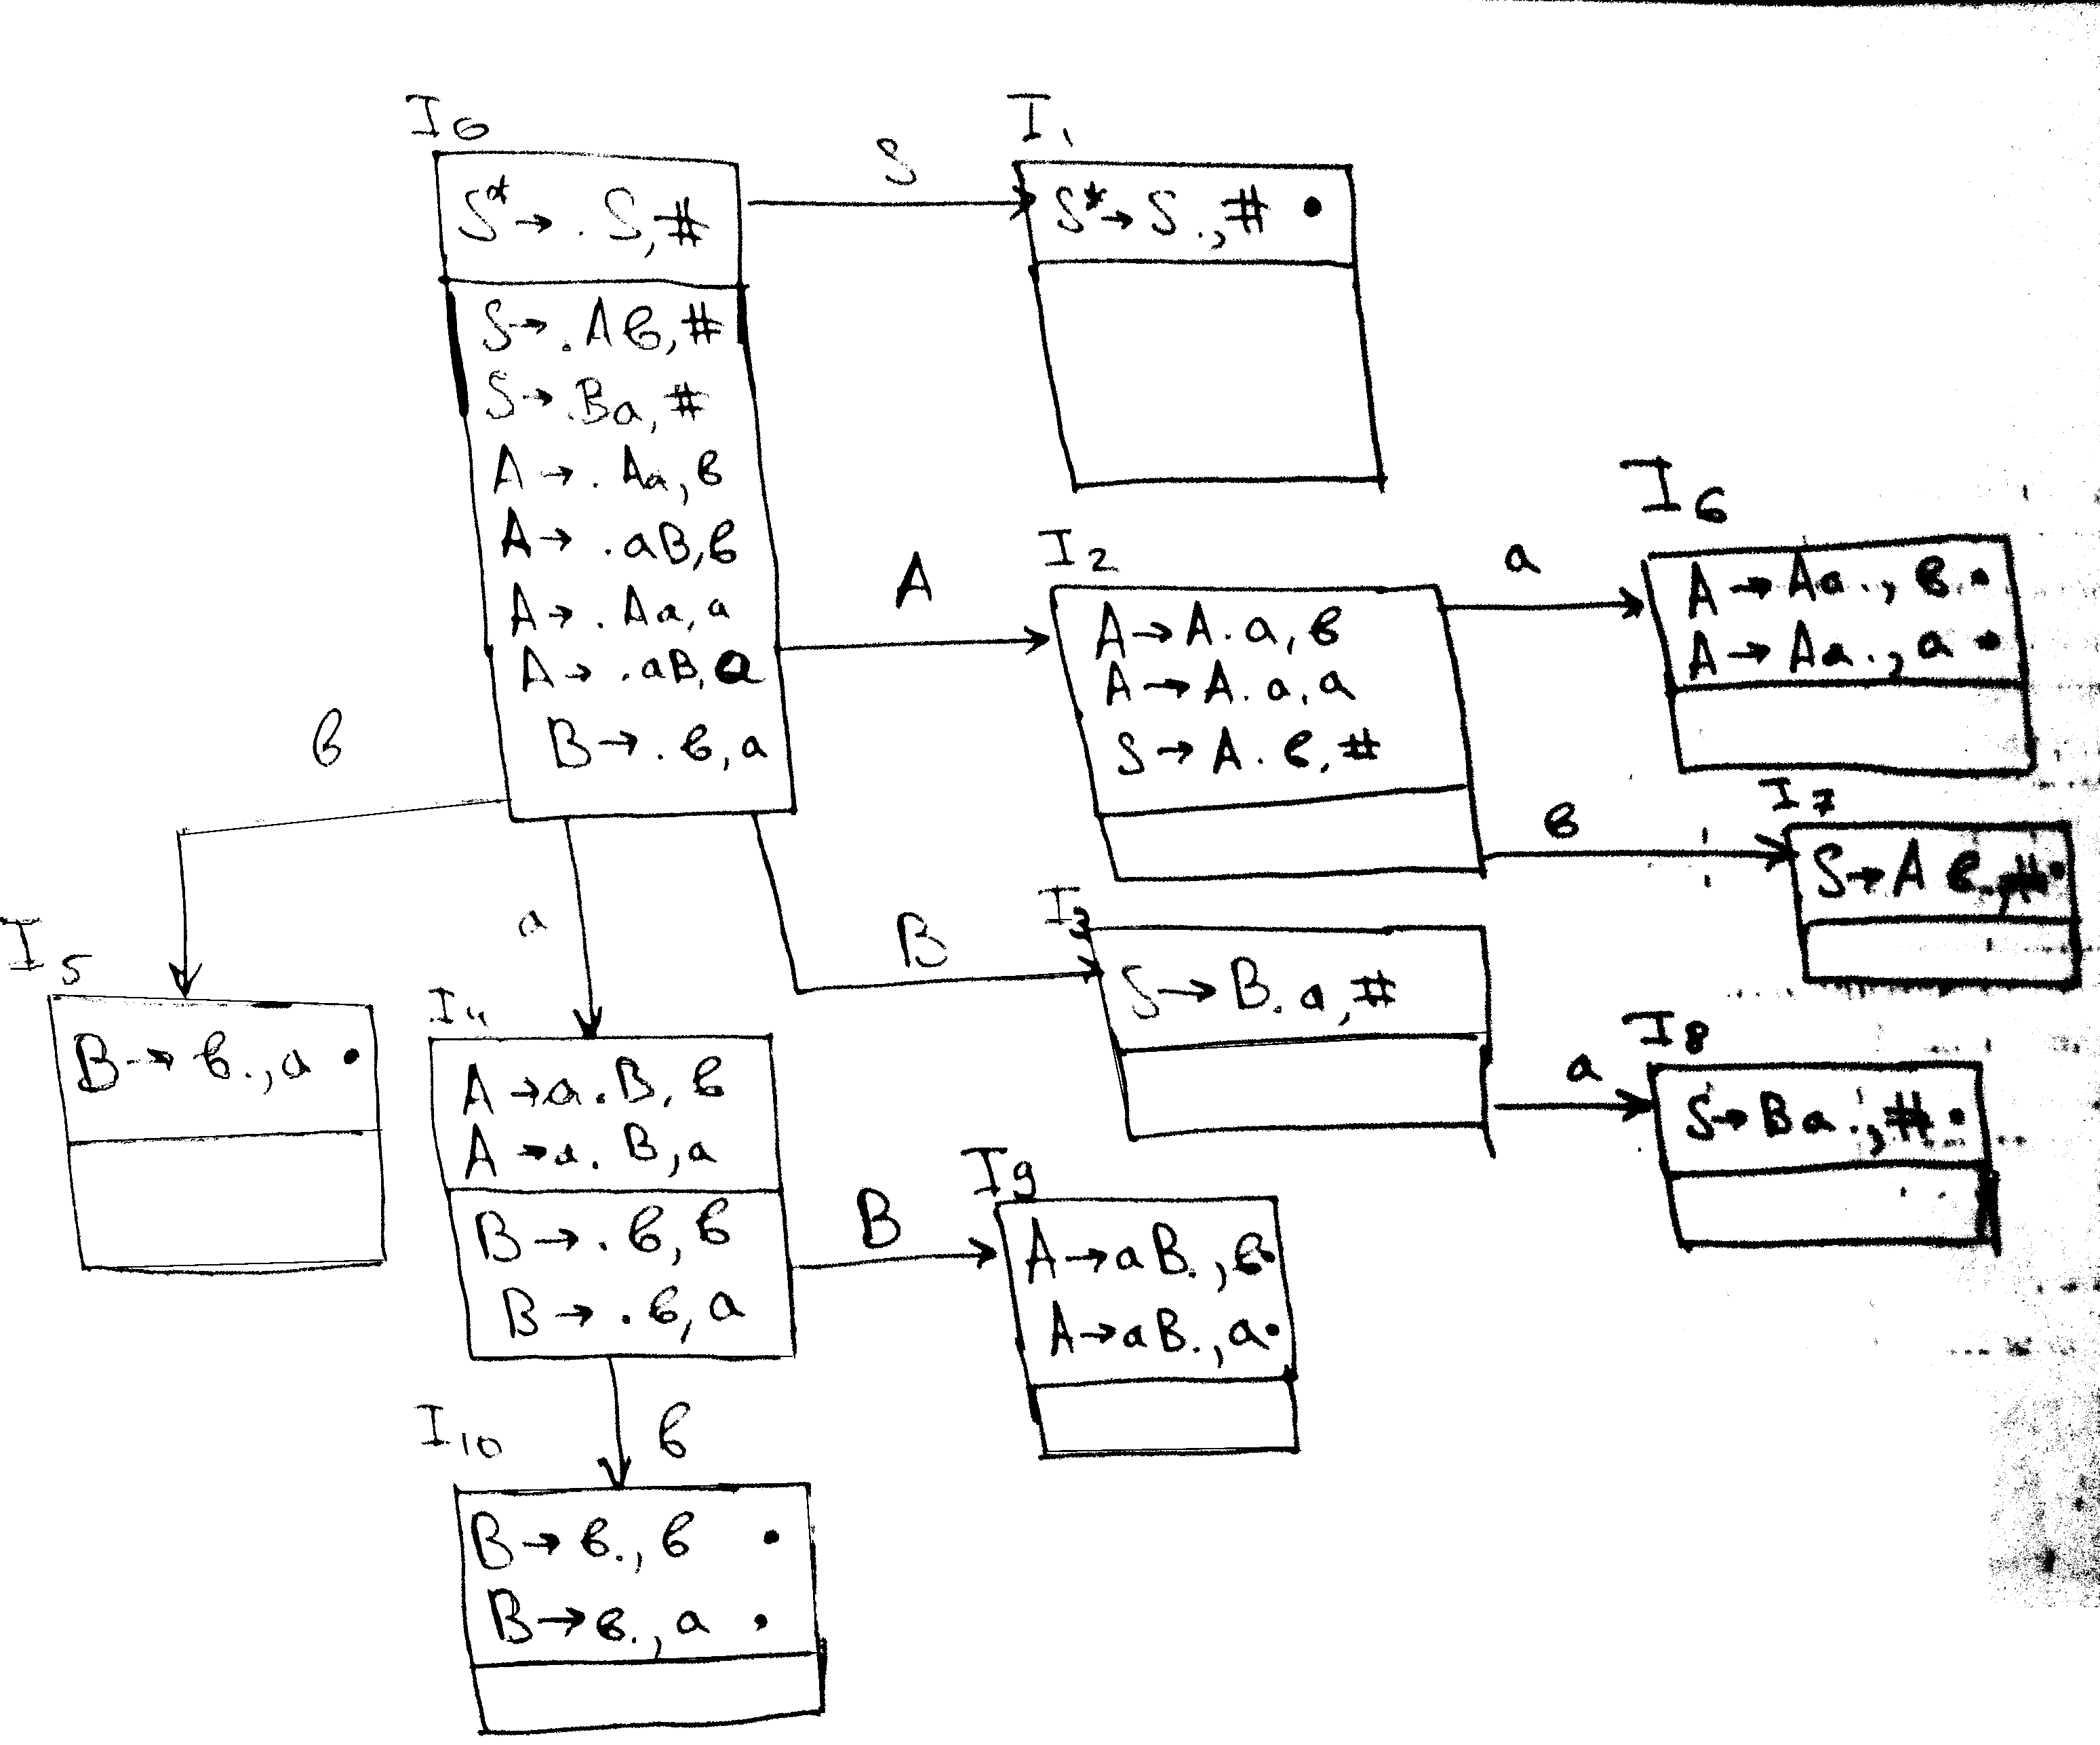
\includegraphics[scale=0.1]{data/pic8_1.png}\\\\
	6) А теперь строим таблицу анализатора. Сразу скажу, что схему с рисунками лучше
	смотреть у Тани: у нее стрелочками помечено, что от каких правил получается.
	Я же привожу только правила.\\
	$\forall I_i \to^{N} I_j$, где $N$ - нетерминал, добавим в таблицу $Goto(I_i,N)=I_j$\\
	$\forall I_i \to^a I_j$, где $a$ - терминал, добавим $Action(I_i, a)=Shift\ I_j$\\
	$\forall I_i$, где есть ситуация вида $A \to \alpha ., b$, добавим 
	$Action(I_i, b) = Reduce\ N(A \to \alpha)$(номер правила)\\
	При этом $Reduce\ N(S^* \to S) = Reduce 0$ записывается как $Accept$\\
	Все остальное - $Error$\\
	Сама таблица:\\\\
	\begin{tabular}{lllllrrrr}
		& $Action$ & $a$ & $b$ & $\#$ & $Goto$ & $S$ & $A$ & $B$ \\
		0 && S4 & S5 &&& 1 & 2 & 3\\
		1 &&&& ACC\\
		2 && S6 & S7\\
		3 && S8\\
		4 &&& S10 &&&&& 9\\
		5 && R5\\
		6 && R3 & R3\\
		7 &&&& R1\\
		8 &&&& R2\\
		9 && R4 & R4\\
		10 && R5 & R5\\
	\end{tabular}\\\\
	7) Разбор цепочки (его по-прежнему лучше посмотреть у Тани)\\
	Все начинается с такого начального состояния:\\
	\begin{tabular}{rcl}
		0 & | & $a_1a_2...a_n\#$
	\end{tabular}\\\\
	Теперь мы будем разбирать цепочку по таблице анализатора, где
	$Reduce$ обозначает выполнение правила грамматики с указанным номером в обратную сторону.\\
	$Shift$ обозначает перенос терминального символа в левый магазин и установку цифры,
	идущей после $S$ туда же.\\
	$Accept$ обозначает принятие цепочки.\\
	Очень важно, чтобы в магазине в конце всегда была цифра!\\
	\begin{tabular}{rcll}
		0 & | & $abab\#$ & [0, a] = S4\\
		0a4 & | & $bab\#$ & [4, b] = S10\\
		0a4b10 & | & $ab\#$ & [10, a] = R5\\
		0a4B & | & $ab\#$ & [4, B] = 9\\
		0a4B9 & | & $ab\#$ & [9, a] = R4\\
		0A & | & $ab\#$ & [0, A] = 2\\
		0A2 & | & $ab\#$ & [2, a] = S6\\
		0A2a6 & | & $b\#$ & [6, b] =  R3\\
		0A & | & $b\#$ & [0, A] = 2\\
		0A2 & | & $b\#$ & [2, b] = S7\\
		0A2b7 & | & $\#$ & [7, $\#$] = R1\\
		0S & | & $\#$ & [0, S] = 1\\
		0S1 & | & $\#$ & [1, $\#$] = ACC
	\end{tabular}\\\\
	Получили Accept - цепочка принадлежит языку, ура!\\
	\newpage
	Чтобы получить дерево разбора, нужно последовательно применять к $S$ правила снизу вверх.\\
	Для слова $abab$ получается такая последовательность: $1, 3, 4, 5$\\
	И само дерево разбора тоже имеется:\\
	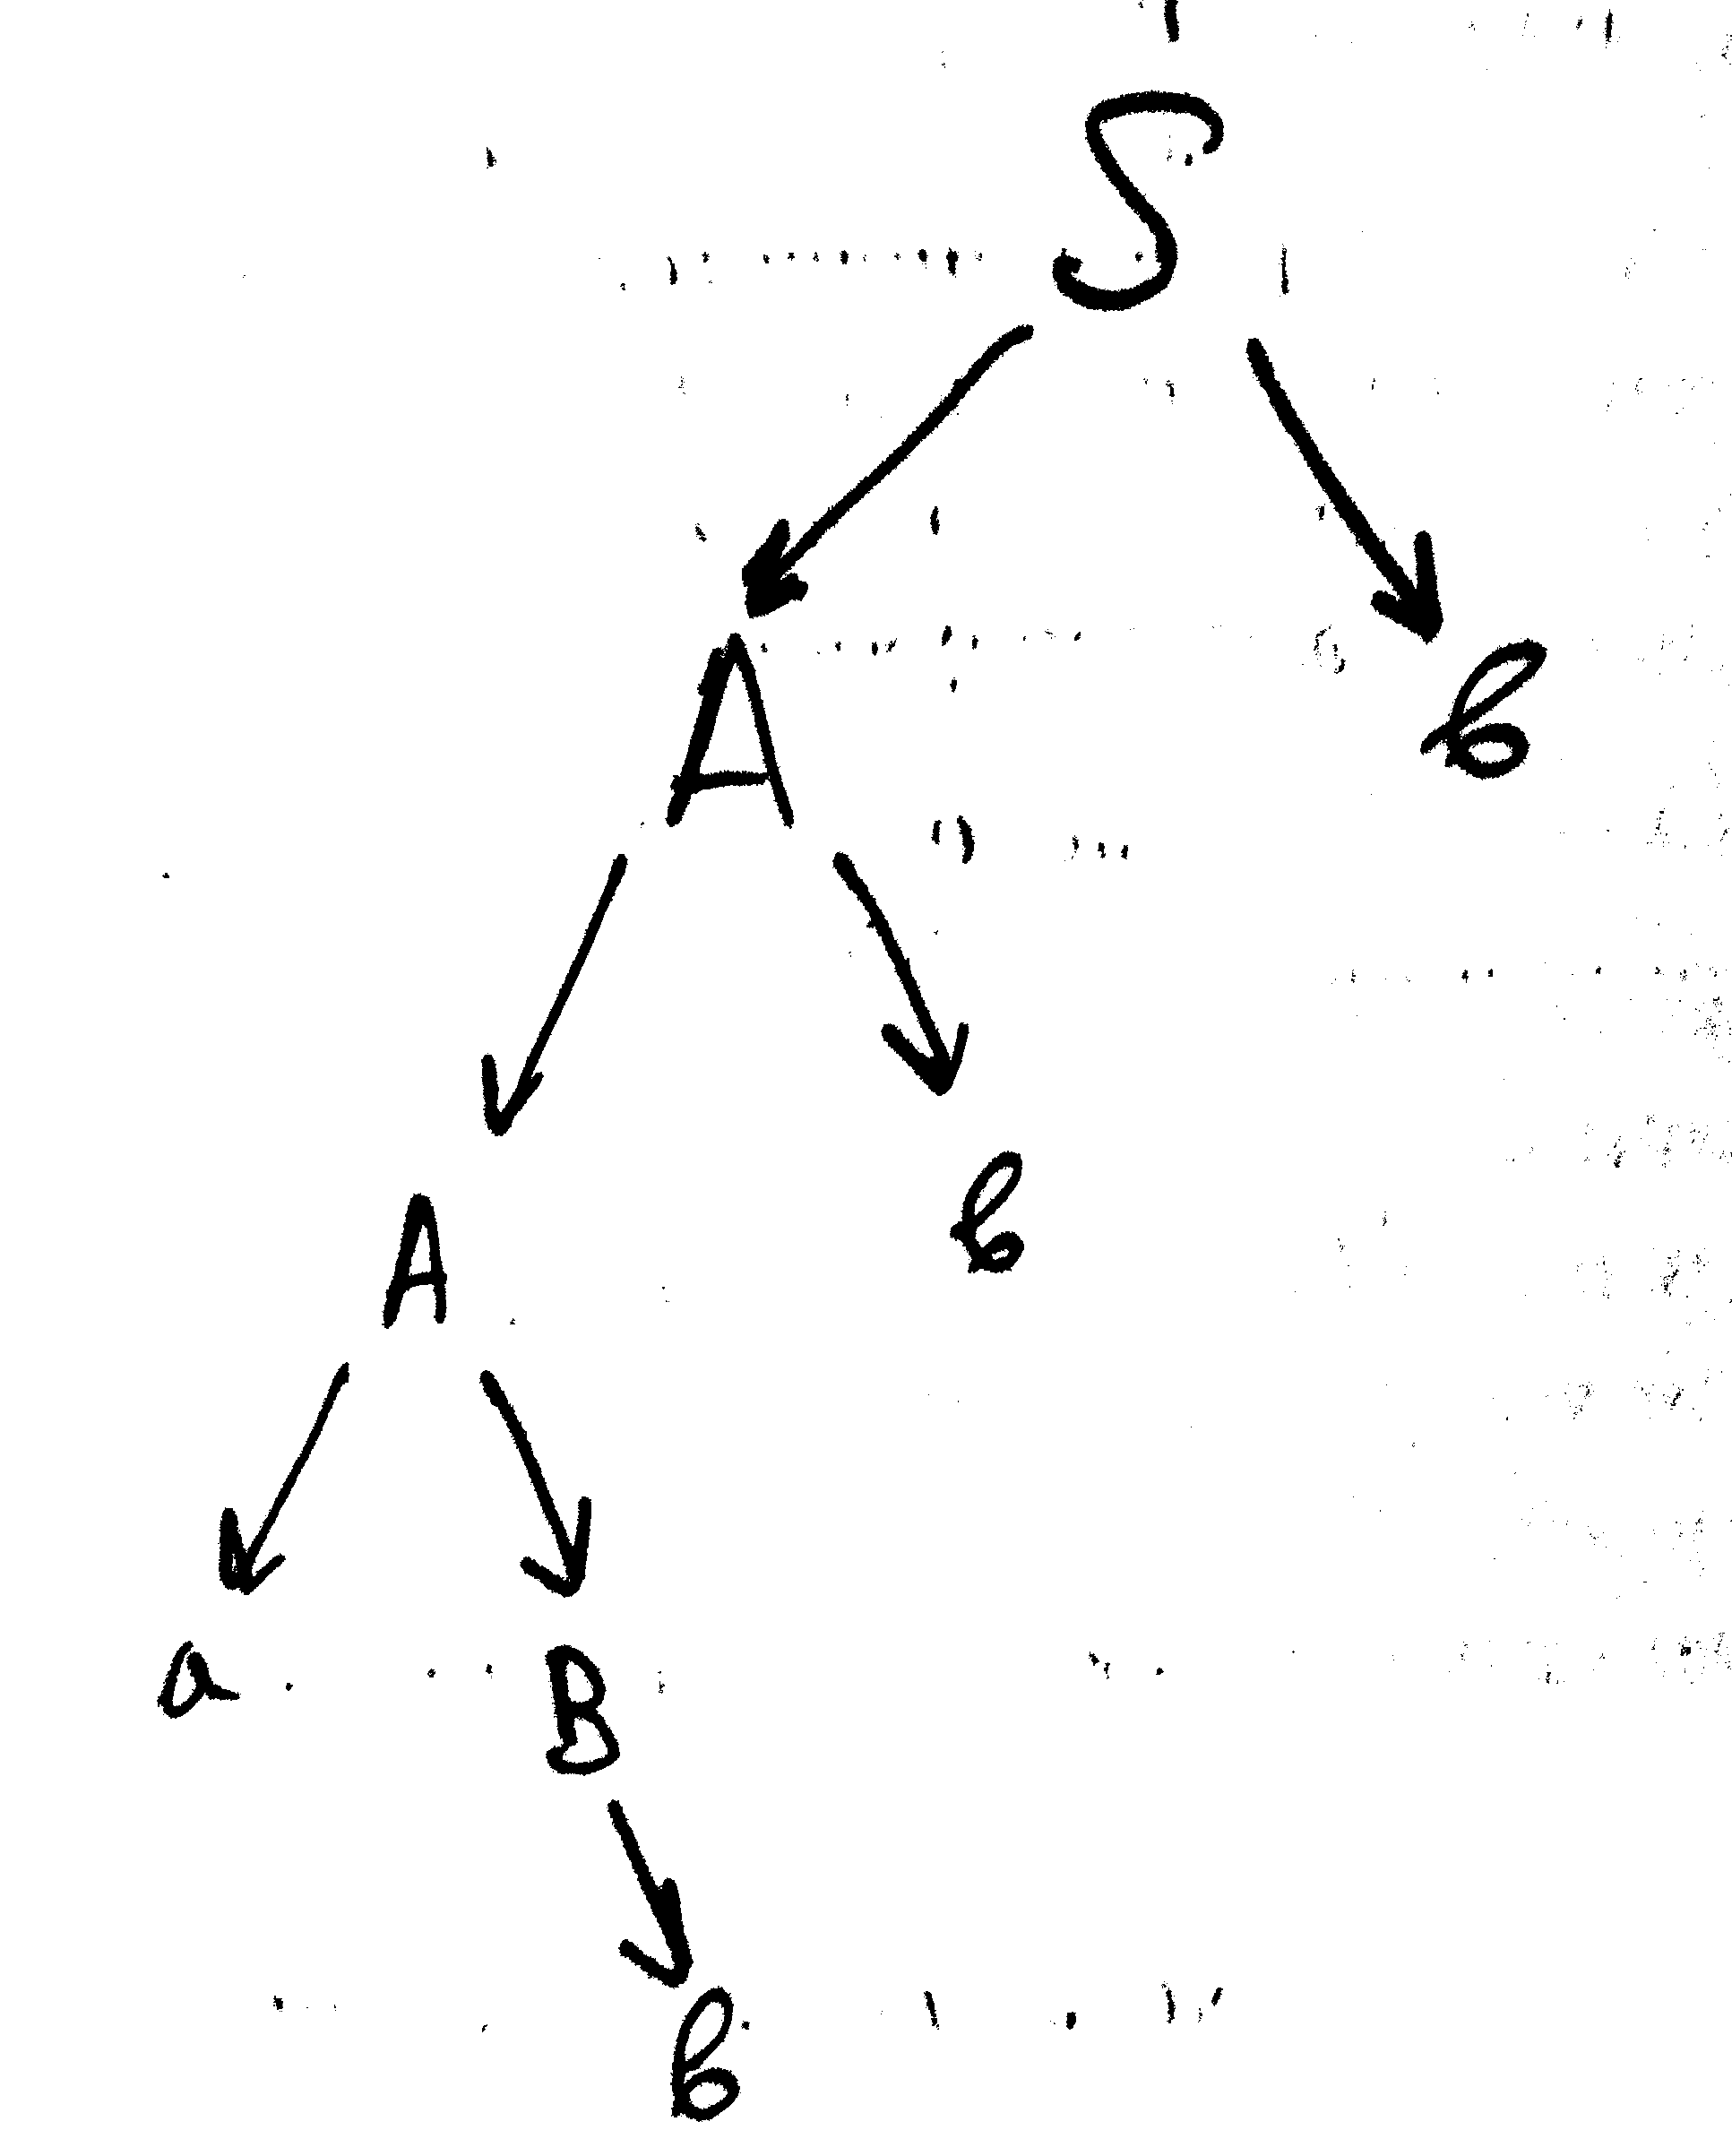
\includegraphics[scale=0.1]{data/pic8_2.png}\\\\
	
	8) По таблице LR(1)-анализатора можно определить, является ли наша грамматика LR(0). Для
	этого должны выполняться следующие условия:\\
	\hspace*{30pt} $Shift$ и $Reduce$ не могут встречаться в одной строке.\\
	\hspace*{30pt} $Reduce$ в одной строке относятся только к одному правилу.\\\\
	\section{Почему это работает}
	Объяснить это очень сложно, но получить какое-то эфемерное понимание всего этого ужаса можно,
	если держать в голове уже изложенную мысль:\\
	$A \to \alpha . B \beta , b$ означает, что мы сейчас работаем на $A$, мы уже обработали
	$\alpha$, в данный момент пытаемся что-то сделать с $B \beta$, а после после разбора всего
	этого великолепия должен остаться символ $b$.\\
	Соответственно переходы по НЕтерминальному символу $Q$ символизируют фразу:
	"Окей, допустим, что мы разобрались с $Q$"\\
	Переходы по терминальному символу $w$ символизируют фразу: "Окей, мы обработали еще и $w$"\\
	А конструкции вида $A \to \alpha ., a$ означает, что существует такой вариант, что
	мы раскрутим нетерминал $A$ по правилу $A \to \alpha$, и при этом справа останется $a$.\\\\
	\section{Ловля ошибок в зародыше}
	Иногда бывает очень полезно понять, что данный вид анализатора не подходит (или была допущена
	ошибка), еще до разбора цепочки. В процессе написания главы про LR-анализаторы я подметил для
	себя такую вещь:\\
	Если вдруг при построении анализатора в одной группе оказались ситуации вида:\\
	$ A \to \alpha . , a$\\
	$ B \to \beta . a , b$\\
	То можно смело сворачиваться или искать ошибку.\\
	Почему?\\
	Потому что первая ситуация будет интерпретирована, как $Reduce N(A \to \alpha )$ по
	символу $a$, а вторая ситуация - как $Shift I_j$ по символу $a$.\\
	Получается конкуренция за символ $a$, значит таблицу анализатора построить в таком виде
	не получится. Если поймать такую ошибку до построения всего анализатора, можно
	сэкономить очень много времени.\\
	Посмотреть на живые примеры таких неудач можно на примере грамматик:\\
	$S^* \to S \\ S \to Sa | a | e$ \\
	Получаются такие конфликтующие ситуации:\\
	$ S \to . a , \#$\\
	$ S \to ., a $\\
	Или более неочевидный пример:\\
	$S^* \to S$ \\
	$S \to AB | b$ \\
	$A \to Aa | e$ \\
	$B \to Bb | b$ \\
	Конфликтующие ситуации там следующие:\\
	$ S \to . b , \# $\\
	$ A \to ., b $\\
	
	Все эти грамматики являются LR(2) грамматиками, потому что есть ситуации, когда мы не
	можем по одному символу из цепочки определить, какое правило нужно применять. В случае
	первой грамматики по символам $aa$ нужно раскручивать правило 1, а по символам $a\#$ - 2.\\
	
	
	
	
	
	\chapter{Лемма о накачке}
	
	Лемма о накачке, а точнее ее отрицание, это, наверное, самый простой способ доказательства
	нерегулярности (как минимум потому, что других я не знаю).\\\\
	Лема звучит следующим образом:\\
	Пусть $L$ - регулярный язык над алфавитом $A$.\\
	Тогда $\exists n \in \mathbb{N}$, что
	$\forall w \in L,\ |w| \geq n\ \exists x,y,z \in A^*: xyz = w, y \neq \epsilon,
	|xy| \leq n$ и $\forall k \geq 0\ xy^kz \in L$\\
	Но это было в общеобразовательных целях. А теперь реально полезная вещь: отрицание
	леммы о накачке.\\\\
	Пусть $L$ - язык над алфавитом $A$.\\
	Если $\forall n \in \mathbb{N}$ найдется такое
	$w \in L,\ |w| \geq n$, что при $\forall x,y,z: xyz = w, |y| \geq 1,\
	|xy| \leq n\ \exists k \in \mathbb{N}: xy^kz \notin L$, тогда язык $L$ нерегулярный.\\\\
	Если простым плебейским языком, то\\
	1) Берем некоторое $n \in \mathbb{N}$.\\
	2) Ему в соответствие ищем особое слово $w \in L$ длины не меньше $n$.\\
	3) Разбиваем его случайным образом на 3 слова $x,y,z$ таким образом, чтобы $y$ был
	непустым, а длина $xy$ не превосходила $n$ (все следующие условия должны выполняться при
	любом возможном разбиении слова $w$).\\
	4) Ищем такое $k \in \mathbb{N}$, чтобы $xy^kz$ не принадлежал языку $L$.\\
	5) Доказываем, что мы сможем найти особое слово для пункта 2 при любом
	$n \in \mathbb{N}$ из пункта 1: $voila$ язык нерегулярный.\\\\
	Часто эта лемма нужна в задачах, где спрашивают "регулярен ли вот этот язык?".\\
	Как несложно догадаться, как правило, он нерегулярен.\\
	\newpage
	Есть довольно неплохой способ (на мой взгляд) быстрой прикидки регулярности языка:
	на язык нужно внимательно смотреть 30 секунд и пытаться придумать для него регулярное
	выражение (только честное каноническое РВ, а не какое-нибудь стероидное из Perl).\\
	Если за 30 секунд пристального взгляда это не удается сделать, значит, язык, скорее
	всего, нерегулярен и можно пробовать раскрутить его через отрицание леммы.\\
	Очень часто даются языки, где количества букв в двух разных местах каким-то образом
	связаны.\\
	Например, $L = a^nb^n$.
	У меня не получилось придумать для него честное каноническое регулярное выражение, поэтому
	применяем лемму.\\
	1) Выбрали и зафиксировали случайное значение $n$.\\
	2) В качестве особого слова возьмем слово $a^nb^n$.\\
	3) При таком выборе особого слова слово $xy$ может быть одним из множества\\
	$\{a, aa,...,a^{n-1},a^n\}$, так как его длина не превосходит $n$. При этом $x$ может быть
	одним из следующих слов $\{a, aa,...,a^{n-1}\}$. Слово $y$ как минимум состоит из
	1 буквы $a$, а слово $x$ - как максимум из $n-1$ буквы $a$.\\
	4) Берем $k=2$. Получаем набор слов, где как минимум $n+1$ букв $a$ и $n$ букв $b$. А это
	слово, очевидно, не принадлежит исходному языку. Радуемся.
	\section{Почему это работает}
	Потому что.\\
	Объяснил?\\
	Хочется реально почитать доказательство?\\
	Если да, можно просто загуглить.\\
	Работает и черт бы с ней.\\\\
	Серьезно.\\
	У нее нет человеческого объяснения.\\
	Как и других лемм/теорем в курсе.\\
	А ты думал, тут сейчас все понятно распишут?\\
	
	\chapter{Немножко полезных советов от человека, который не сдал}
	1) Кажду задачу можно решать с чуть-чуть различающимися обозначениями. Попробуйте найти
	удобную для себя нотацию к каждой задаче и отработайте ее.\\
	2) Используйте цветные ручки/карандаши. Нет, это не гейство, это вынужденный гомосексуализм.
	Размечайте цветом все, что нужно потом будет быстро друг от друга отличать. Это повышает
	скорость обработки в дальнейшем, а главное - повышает точность.\\
	Из того, что могу подсказать я:\\
	$firstpos,\ followpos$ в дереве РВ.\\
	Начальные, конечные состояния автоматов.\\
	Переходы по терминалам/нетерминалам в LR-анализаторах.\\
	$Reduce$ ситуации в LR-анализаторах.\\
	3) Используйте более короткую и более емкую запись. Ни в коем случае не рисуйте автоматы так,
	как я рисовал их для этой методички: я изрядно заебался штриховать эти круги по 8 секунд
	каждый, но делал это, чтобы было как можно лучше видно в ЧБ исполнении. На мой взгляд
	достаточно поставить звездочку у конечного состояния (или, как уже предлагалось выше,
	использовать цвета)\\
	Очень не советую полность расписывать похожие ситуации в LR-анализаторах так\\
	$ A \to .,a \\ A \to .,b \\ A \to .,\#$\\
	Они вполне неплохо помещается в таком виде\\
	$A \to .,ab\#$ (но опять же, к такой форме нужно чуть-чуть привыкнуть, чтобы не косячить)\\
	4) Берегите себя и своих близких.
	\chapter{Благодарности}
	Спасибо корешам, перед которыми я в свое время зарекнулся написать это все.\\
	Спасибо Владиславу Грубову и Вадиму Глазкову за стилистические замечания (да, раньше
	язык был еще хуже) и помощь в поиске ответов на вопросы по сути предмета.\\
	Спасибо Михаилу Валентиновичу Федотову за то, что этот потрясающий курс преподается в
	стенах факультета ВМК.\\\\
	
	
	
	
	
	
	
\end{document}
